\chapter[Fake Factor Method]{Fake Factor Method to estimate Background from Lepton Misidentifications}
\label{app:fake-factor-method}
This section describes how the background from lepton misidentifications is estimated using the fake factor method.

\section{Control sample definition}
The control sample is distinguished from the nominal selection by using an alternative lepton selection.
One of the two prompt lepton candidates is required to fail the full identification criteria defined in \cref{sec:object-selection} but satisfies a looser set of criteria, referred to as \emph{anti-identified} lepton.
%\Cref{tab:leptonID} summarizes the lepton selections for fully identified and anti-identified leptons. 
%Paper
%They are estimated using a data-driven technique8 where 464 control samples are established in which all nominal selections are applied with the exception that one of 465 the two lepton candidates fails to meet the full identification criteria defined in Section 4, but satisfies a 466 looser set of identification criteria (referred to as an anti-identified lepton).
% \begin{table}
%     \scalebox{0.77}{
%         \begin{tabular}{c|c||c|c}
%             \toprule
%             % \dbline
%             \multicolumn{2}{c||}{Electron}                                       & \multicolumn{2}{c}{Muon}                                                                                                      \\
%             identified                                                           & anti-identified                                  & identified                          & anti-identified                      \\
%             \midrule
%             % \sgline
%             \multicolumn{2}{c||}{$\pt  > 15 \mathrm{GeV}$}                     & \multicolumn{2}{c}{$\pt   > 15 \mathrm{GeV}$ }                                                                              \\
%             \multicolumn{2}{c||}{$|\eta|  <2.47$,excluding  $1.37<|\eta|< 1.52$} & \multicolumn{2}{c}{$|\eta|  <2.5$}                                                                                            \\
%             \multicolumn{2}{c||}{$|z_{0}\sin\theta|<0.5$ mm }                    & \multicolumn{2}{c}{$|z_{0}\sin\theta|<0.5$ mm }                                                                               \\
%             \multicolumn{2}{c||}{$|d_{0}|/\sigma(d_{0})<5$ }                     & $|d_{0}|/\sigma(d_{0}) <  3$                     & $|d_{0}|/\sigma(d_{0}) <  15$                                              \\
%             Pass LHTight if $\pt < 25 \;\mathrm{GeV}$                            & \multirow{3}{*}{Pass LHLoose}                    & \multirow{3}{*}{Pass Quality Tight} & \multirow{3}{*}{Pass Quality Medium} \\
%             Pass LHMedium if $\pt > 25 \;\mathrm{GeV}$                           &                                                  &                                     &                                      \\
%             Pass FCTight isolation                                               &                                                  & Pass FCTight isolation              &                                      \\
%             \multicolumn{2}{c||}{ {\scshape Author} $= 1$}                       &                                                  &                                                                            \\
%                                                                                  & Veto against identified electron                 &                                     & Veto against identified muon         \\
%             % \dbline
%             \bottomrule
%         \end{tabular}
%     }
%     \caption{Selection criteria for fully identified and anti-identified leptons.}
%     \label{tab:leptonID}
% \end{table}

\section{Extrapolation to analysis regions}
The contributions of backgrounds with misidentified leptons (Mis-Id background) are estimated by subtracting the  expected number of events in the control sample with the expected contribution from processes with two true, prompt leptons, and then multiplying it with the corresponding fake factors.
The full expression can be written as,
\begin{equation}
    \label{app:eq:fake-estimation}
    N_{\text{id,id}}^{\text{Mis-Id}} = FF \left( N_{\text{id,\sout{id}}}^{\text{data}} - N_{\text{id,\sout{id}}}^{\text{2 true prompt}} \right) - FF_1FF_2 \left( N_{\text{\sout{id},\sout{id}}}^{\text{data}} - N_{\text{\sout{id},\sout{id}}}^{\text{2 true prompt}} \right),
\end{equation}
where $N_{\text{id,\sout{id}}}^{\text{data}}$ and $N_{\text{\sout{id},\sout{id}}}^{\text{data}}$ are, respectively, the number of expected events with one or two anti-identified leptons measured in the control data sample, and $N_{\text{id,\sout{id}}}^{\text{2 true prompt}}$ and $N_{\text{\sout{id},\sout{id}}}^{\text{2 true prompt}}$ are, respectively, the number of expected events with two true, prompt leptons measured in simulated event samples.
The fake factors $FF$ and $FF_{1/2}$ are applied according to which leptons are anti-identified, that is, whether it is the electron, the muon, or both.
They are dependent on the \pT of the anti-identified lepton and, in the case of a misidentified muon, $\abseta$, i.e. $FF \to FF(\pT, \abseta)$.
The second term on the right-hand side of \cref{app:eq:fake-estimation} provides a correction for events where both of the leptons are misidentified, a contribution that is double-counted in the first term. A rigorous mathematical derivation of \cref{app:eq:fake-estimation} goes beyond the scope of this thesis and the interested reader is referred to \ccite{HIGG-2013-13,HIGG-2016-07,KonstiThesis}.

\section{Derivation of nominal fake factors in \Zjets-enriched sample}
\label{app:subsubsec:zjets-ffs}
The fake factors are estimated using a data sample enriched in \Zjets events and a three-lepton selection (referred to as \Zjets selection), that targets events with two leptons originating from the $Z$ boson decay and a jet that serves as candidate for being misidentified as a lepton (referred to as Mis-Id candidate).
%A three-lepton selection, referred to as \Zjets selection, is therefore applied. 
All leptons must satisfy \ptGT{15}\,GeV.
The two leptons of opposite charge and same flavor that qualify as $Z$ decay particles are chosen to be the ones that have an invariant mass close the $Z$ boson mass. If these two leptons are electrons (muons), a requirement of $80 < m_{ee} < 110\,$GeV ($70 < m_{\mu\mu} < 110\,$GeV) is applied.
The two leptons are required to be fully identified except of the isolation requirement that is loosened to the ``Loose'' working point selections and the identification working point that is modified to ``Loose'' for electrons and ``Medium'' for muons.
Relaxing these criteria allows for a better statistical precision in the fake factor derivation.
In addition, at least one of the two leptons must be associated to the online object that triggered the single-lepton trigger used in the analysis as described in \cref{sec:data-mc-samples}.
If more than one pair of leptons satisfies these requirements, the pair with the invariant mass closest to the $Z$ boson mass is chosen.
The respective other lepton in the event serves as the Mis-Id candidate.
The fake factor is then defined as the ratio of events, where this Mis-Id candidate is fully identified, $N_{\text{id}}^{\text{data}}$, and anti-identified, $N_{\text{\sout{id}}}^{\text{data}}$, each time subtracting the expected number of events with three true, prompt leptons that are not originating from \Zjets processes,
\begin{equation}
    \label{app:eq:ff}
    FF = \frac{ N_{\text{id}}^{\text{data}} - N_{\text{id}}^{\text{non-\Zjets}}}{N_{\text{\sout{id}}}^{\text{data}} - N_{\text{\sout{id}}}^{\text{non-\Zjets}}}.
\end{equation}
The events with three true, prompt leptons, $N_{\text{id/\sout{id}}}^{\text{non-Zjets}}$, are estimated using simulated samples and are dominated by leptonically decaying $WZ$ production.
To reduce the contamination of this process, a requirement of $m_T^W = \sqrt{2E^{\textrm{miss}}_\textrm{T} E^{\text{Mis-Id cand.}}_\textrm{T} (1-\cos\phi)} < 50\;\textrm{GeV}$ is additionally applied in the \Zjets selection.
The resulting fake factors are summarized in \cref{app:tab:ZjetsFF-uncertainties}.
The fake factors are derived separately for electrons and muons. The electron fake factors are split into four different \pT bins and are measured inclusively for the entire \abseta range.
The muon fake factors are also derived in four \pT bins and two \abseta regions \absetaST{1.05} and \absetaGT{1.05}. The value of the last \pT bin with \ptGT{50}\,GeV is derived by an extrapolation from the respective previous bin, due to the limited statistical precision at high \pT.
\begin{table}[ht]
    \begin{center}
        % This file was created on 2020-06-04 06:11:19 by the script makeSummaryTable.py.
\begin{tabular}{c|c|c|c|c|c}
    \toprule
    Kinematic Region                        & Nominal & Statistical & $EW$ Subtraction & flavor composition & Total \\
    ($|\eta|$ and $\pt$ range)              &       &             &                &                    &       \\
    \midrule
    \multicolumn{1}{l|}{\textbf{Electron}} &       &             &                &                    &       \\
    \multicolumn{1}{l|}{$0<|\eta|<2.5$}   &       &             &                &                    &       \\
    \multicolumn{1}{r|}{$15-20$\,GeV}    & 0.076 & 6.2         & 3.9            & 7.5                & 10    \\
    \multicolumn{1}{r|}{$20-25$\,GeV}    & 0.086 & 11          & 8.1            & 31                 & 34    \\
    \multicolumn{1}{r|}{$25-35$\,GeV}    & 0.14  & 13          & 14             & 7.4                & 20    \\
    \multicolumn{1}{r|}{$> 35$\,GeV} & 0.21  & 12          & 25             & 21                 & 35    \\
    \midrule
    \multicolumn{1}{l|}{\textbf{Muon}}     &       &             &                &                    &       \\
    \multicolumn{1}{l|}{$0<|\eta|<1.05$}  &       &             &                &                    &       \\
    \multicolumn{1}{r|}{$15-20$\,GeV}    & 0.042 & 8.4         & 7.1            & 8.1                & 14    \\
    \multicolumn{1}{r|}{$20-25$\,GeV}    & 0.017 & 35          & 34             & 11                 & 50    \\
    \multicolumn{1}{r|}{$25-50$\,GeV}    & 0.026 & 39          & 58             & 11                 & 71    \\
    \multicolumn{1}{r|}{$50-\infty$\,GeV}  & 0.043 & 47          & 58             & 11                 & 75    \\
    \multicolumn{1}{l|}{$1.05<|\eta|<2.5$}  &       &             &                &                    &       \\
    \multicolumn{1}{r|}{$15-20$\,GeV}    & 0.060 & 6.7         & 5.3            & 8.1                & 12    \\
    \multicolumn{1}{r|}{$20-25$\,GeV}    & 0.042 & 17          & 14             & 11                 & 25    \\
    \multicolumn{1}{r|}{$25-50$\,GeV}    & 0.065 & 19          & 28             & 11                 & 36    \\
    \multicolumn{1}{r|}{$> 50$\,GeV}  & 0.11  & 32          & 28             & 11                 & 44    \\
    \bottomrule
    \end{tabular}
    
    \end{center}
    \caption[Summary of the fake factors from the $Z$+jets estimate with uncertainties.]{Summary of the fake factors from the $Z$+jets estimate with uncertainties. All uncertainties are quoted in percent on the nominal value. More information on the different uncertainty components is given in the text.
        % \textit{Value} denotes the nominal fake factor value. \textit{Statistical} denotes the statistical uncertainties on the fake factors including the extrapolation uncertainty for the highest muon \pT bin. \textit{EW Subtraction} denotes the uncertainty due to the electroweak backgrounds that enter the $Z$+jets fake factor estimate. \textit{Sample Composition} denotes the uncertainty that accounts for differences in fake factors between $Z$+jets and $W$+jets processes, and includes both statistical and systematic uncertainty on the correction factors. The column \textit{Total} sums all individual contributions in quadrature to give an overview of the total uncertainty of the fake factor. In the fit, however, the EW subtraction and sample composition uncertainties are treated as correlated between different bins, while the statistical uncertainty is uncorrelated.
    }
    \label{app:tab:ZjetsFF-uncertainties}
    % Nominal values, statistical uncertainties and EWSUBTR uncertainties produced on tag kon_improveZjetsFFStats_v2
\end{table}

\section{Derivation of triggered fake factors in dijet-enriched sample}
The events in the control sample are selected based on one of three trigger decisions: The dilepton trigger is fired, only one single-lepton trigger is fired by the fully identified lepton, or only one single-lepton trigger is fired by the anti-identified lepton.
For events falling into the latter category, the trigger requirements are more stringent than the definition of the anti-identified lepton, leading to a bias in the event yield.
Although the number of events in that category accounts for only $\mathcal{O}(1\%$) or less and the impact on the analysis is therefore small, specific so-called \emph{triggered fake factors} subject to the same bias are derived for these types of events. This is achieved by considering a data sample where the anti-identified lepton fires the single-lepton trigger.
    Applying such a requirement in addition to the \Zjets selection, however, leads to an insufficient event yield to derive reasonable fake factors. The triggered fake factors are therefore derived in a sample enriched in dijet events.
    The dijet selection requires each event to have at least one Mis-Id candidate with \ptGT{15}~\,~GeV and one jet with \ptGT{25}~\,~GeV. To ensure a back-to-back topology between the lepton and the jet, the two objects must have an angular separation $\Delta \phi(\text{lep}, \text{jet}) > 2.5$.
    In order to suppress the contamination from non-dijet processes, mostly coming from \Wjets processes, the events are required to have $\MET < 30$\,GeV and the transverse mass between the lepton and the missing transverse energy must satisfy $m_T < 60\,$GeV.
    The fake factors are then derived analogous to \cref{app:eq:ff}, but subtracting non-dijet events in the numerator and denominator.
    % The overall number of events that are subject to a trigger bias is very small.
    % \begin{equation}
    %     \label{app:eq:ff-dijet}
    %     FF^{\text{dijet}} = \frac{ N_{\text{id}}^{\text{data}} - N_{\text{id}}^{\text{non-dijet}}}{N_{\text{\sout{id}}}^{\text{data}} - N_{\text{\sout{id}}}^{\text{non-dijet}}}.
    % \end{equation}


\section{Corrections and uncertainties}
Uncertainties in the estimation of the Mis-Id background in the analysis are account for via uncertainties in the fake factors.
The fake factor uncertainties can be grouped into three main components: statistical uncertainties, uncertainties in the normalization of non-\Zjets processes that are subtracted in \cref{app:eq:ff}, and uncertainties due to the different flavor composition of jets in \Zjets processes compared to \Wjets processes.
The latter uncertainty arises due to a correction that must be applied to the fake factors derived in \Zjets events.
Each uncertainty component and correction is discussed below, and their impact is summarized in \cref{app:tab:ZjetsFF-uncertainties}.


\subsection{Statistical uncertainty}
The statistical uncertainties refer to the uncertainties in the data sample used to derive the fake factors as shown in \cref{app:eq:ff}.

\subsection{$EW$ subtraction uncertainty}
The contribution of non-\Zjets processes subtracted in \cref{app:eq:ff} is primarily due to $WZ$ processes but also $ZZ$ and $Z\gamma$ processes can enter the \Zjets selection.
Theoretical uncertainties in the normalization of these processes are derived and propagated, leading to systematic uncertainties in the fake factor.
In order to reduce the impact of theoretical uncertainties associated to the $WZ$ process, the normalization of the $WZ$ contribution is extracted from a control region. The CR is defined by inverting the $m_T^W$ selection to $m_T^W > 50\,$GeV and requiring the Mis-Id candidate to pass the full identification criteria. This region is very pure in $WZ$ events so that a precise normalization factor of $0.99 \pm 0.01$ can be extracted and applied in the \Zjets selection. The impact of the uncertainties affecting similarly the normalization in the \Zjets selection and the $WZ$ CR selection can thus be reduced.

    % Uncertainties associated to the $WZ$ process and their impact on the fake factors are estimated with simulated samples and propagated to the final analysis results.
    % Together they are referred to as the $EW$ subtraction uncertainty.

\subsection{Correction factor and flavor composition uncertainty}
The nominal fake factors are derived in \Zjets candidate events, because of the ability to define a region very pure in \Zjets events with little contamination from other processes. However, the dominant contribution to the Mis-Id background in this analysis comes from \Wjets processes.
Because the flavor of the quarks that give rise to the jets in \Zjets processes differs on average from that in \Wjets processes, and the quark flavor is expected to affect the misidentification rate, a \emph{correction factor} (CF) is applied to the nominal fake factors.
The CF is given as the ratio of fake factors derived in simulated \Wjets events and \Zjets events,
\begin{equation}
    CF = \frac{FF^{\Wjets}}{FF^{\Zjets}},
\end{equation}
and applied as a multiplicative factor to the fake factor,
\begin{equation}
    FF^{\Wjets} = FF^{\Zjets} \times CF.
\end{equation}
The same selections are applied to the simulated samples as in the three-lepton \Zjets selection and the CF is derived separately for misidentified electrons and muons.
The systematic uncertainties associated to the CF are derived by using an alternative MC generator and summed in quadrature with the statistical uncertainty in the simulated \Wjets and \Zjets sample.


\FloatBarrier
\chapter{Development of the VBF DNN}
\label{app:chap:DNN}
\section{Software suite}
\label{app:dnn:software-suite}
The software used for the development of the DNN is based on industry-standard open-source ML libraries.
The entire workflow is based on Docker images~\cite{merkel2014docker} that provide the necessary packages that are all built with a Python~\cite{10.5555/1593511} frontend. The simulated MC samples provided centrally within the ATLAS collaboration are first transformed in order to remove the ATLAS software dependencies and make them easily useable with open-source ML libraries. The data are then stored in hdf5~\cite{fortner1998hdf} format, and handled with the numpy~\cite{2020NumPy-Array} and pandas~\cite{mckinney2010data} packages. The training is performed using Keras~\cite{chollet2015keras} and TensorFlow~\cite{abadi2016tensorflow} with the majority of the frontend provided by the FreeForestML~\cite{FreeForestML} library.
The scikit-learn~\cite{pedregosa2011scikit} library is used for data preprocessing, and the matplotlib~\cite{hunter2007matplotlib} package as well as the uhepp~\cite{UheppFrank} package are used for data visualization. The final DNN model is stored in JSON~\cite{pezoa2016foundations} format and deployed in the \HWW\ analysis using the C++ based LightWeight Tagger Neural Network (lwtnn)~\cite{daniel_hay_guest_2019_3249317} package.

\section{Optimization studies}
\label{app:dnn:opt-studies}
Several optimization studies for the VBF DNN were performed during the course of the author's PhD studies.
The following studies were performed with an earlier version of the DNN training setup, including an earlier version of the training data. For this reason, the absolute values of $Z0_{\mathrm{VBF}}$ (\cref{eq:significance-performance-metric}) are not necessarily comparable with other results presented in this thesis. However, the conclusions hold because the results were compared against each other.

\subsection{Study of DNN input variables}
Many sets of observables were studied for use as DNN input variables.
As baseline, the set of variables that was used in the BDT-based analysis of the previous iteration of the \HWW\ measurement \cite{HIGG-2016-07} is chosen, comprising in total 8 variables.
The performances of DNN models using a different number of variables are shown in \cref{tab:input-var-opt}.
Comparing the baseline to the results labelled ``S1'' shows significant improvements. This is an indication that the DNN exploits the correlations between the single $m_{\ell_\alpha j_\beta}$ (with $\alpha, \beta = 1, 2$) and other observables.
Although the discrimination power of \pTjone and \pTjtwo in linear dimension is limited, they also introduce a significant performance improvement when being included (``S2''). The same is true for the \pTjthree observable (``S3''), which adds information about whether a third jet is present in the event.
The final variable that was added and showed improvements is \METSig (``S4''). This observable has only recently been developed for use in the ATLAS collaboration \cite{ATLAS-CONF-2018-038} and is a strong discriminant between events with real undetected high-\pT particles and events where the \MET is the result of resolution effects.
Overall, the significance \ZVBF improves by a maximum of almost 50\% when comparing the baseline with the best performing set.
These results motivate the use of 15 input variables that correspond to the set labelled ``S4'' in \cref{tab:input-var-opt}.
In addition to the comparisons shown, several other observables were studied but did not lead to further improvements.
These tests included (i) using the $C_\ell$ observable separately instead of the sum for both leptons, $\lepetacent$, (ii) using \MET instead of \METSig, and (iii) using the \pT of both leptons on top of the other 15 variables.
Furthermore, the performance was studied of DNN models trained with all 15 variables except one. It was seen, that all chosen 15 variables provide discrimination power, although dropping highly correlated observables such as \mjj and \dyjj did not show large performance losses.

The physics-motivated optimization of the input variables was followed by the rather technical optimization of the neural-network architecture.
The performances of different setups are shown in \cref{tab:architecture-opt}. All results are very comparable to each other. Among the best performing architectures, the one with the least layers is chosen, which corresponds to the architecture labelled ``A4''. The results were produced with the set of variables labelled ``S3'' in \cref{tab:input-var-opt}.
% The reader is also referred to \cref{app:dnn:erratum} for another insight on the network architecture.

\begin{table}[h]
    \centering
    \small
    \begin{tabular}{ l l | r}
        \toprule
        Identifier & Input Variables                                                                                         & \ZVBF \\
        \midrule
        Baseline   & \mjj, \dyjj, \lepetacent, \dphill, \mll, \mT, \pttot, $\sum_{\alpha,\beta=1,2} m_{\ell_\alpha j_\beta}$ & 7.7           \\
        S1         & Baseline w/ separate \mlonejone, \mlonejtwo, \mltwojone, \mltwojtwo,                                    & 8.57          \\
        S2         & S1 + \pTjone, \pTjtwo                                                                                   & 9.55          \\
        S3         & S2 + \pTjthree                                                                                          & 10.92         \\
        S4         & S3 + \METSig                                                                                            & 11.5          \\
        \bottomrule
    \end{tabular}
    \caption{Comparison of the significance metric \ZVBF for DNN models trained with different sets of input variables. The metric is evaluated using the validation set of a 2-fold cross-validation procedure.}
    \label{tab:input-var-opt}
\end{table}

\begin{table}[h]
    \centering
    \small
    \begin{tabular}{ l l | r}
        \toprule
        Identifier & Hidden layers                      & \ZVBF \\
        \midrule
        A1         & {32, 16, 8}                        & 10.4          \\
        A2         & {64, 32, 24, 16, 8}                & 10.6          \\
        A3         & {128, 64, 32, 24, 16, 8}           & 10.7          \\
        A4         & {256, 128, 64, 32, 24, 16, 8}      & 10.8          \\
        A5         & {128, 128, 64, 64}                 & 10.5          \\
        A6         & {512, 256, 128, 64, 32, 24, 16, 8} & 10.8          \\
        \bottomrule
    \end{tabular}
    \caption{Comparison of the significance metric \ZVBF for DNN models using different architectures. The metric is evaluated using the validation set of a 2-fold cross-validation procedure.}
    \label{tab:architecture-opt}
\end{table}


\subsection{Optimization of the EW~$WW$ training fraction}
\label{app:sec:ewww-sample-fraction-optimization}
In a previous iteration of the VBF, \HWW\ analysis it was found that theoretical uncertainties related to particular processes dominate the final measurement uncertainties. In particular EW~$WW$ processes that mimic the VBF signal signature contributed significantly in the highest DNN bin, which lead to large uncertainties.
This prompted a change in the training procedure that places more emphasis on suppressing the EW~$WW$ background by increasing the training fraction, $S_\mathrm{frac}$, of the EW~$WW$ sample in the training.
In addition, an adapted performance metric, \ZVBFunc, was introduced to take into account theoretical uncertainties on the different processes when comparing different DNN trainings.
For this metric, approximate uncertainties are assumed for each process, see \cref{tab:rough-uncertainties}, by studying the total systematic uncertainties on the expected number of events in the highest DNN bin. They are included in the calculation of $Z0(s, b, \sigma)$ (\cref{eq:simple-sign}) via the $\sigma$ parameter.

The results of this optimization of the VBF DNN are shown by means of the expected number of events in the highest DNN bin in \cref{fig:bkg-fractions}. The contributions for each process without and with an increased training fraction for the EW~$WW$ processes are displayed.
The goal of this optimization is to achieve approximately equal number of expected events in the highest DNN bin for the dominant background processes with large uncertainties (which are ggF, EW~$WW$, $WW$, and \ttbar, see \cref{tab:rough-uncertainties}).
This is expected to prove beneficial when combining the uncertainties in the statistical analysis, compared to a scenario where one of the backgrounds dominates.
Due to this change, the final measurement uncertainties of the VBF, \HWW\ production cross section were reduced by roughly 5\%. 

The details of this study that lead to the final choice of the EW~$WW$ training fraction are visualized in \cref{fig:ew-fraction-scan}. All significances indicated are calculated prior to the statistical analysis and correspond to the \ZVBF as described in \cref{subsec:performance-metrics} (with two different binnings) and \ZVBFunc as described above. 
It can be seen that the EW~$WW$ fraction of the total background in the highest DNN bin (blue points; right axis) decreases as the training fraction used for EW~$WW$ processes in the training is increased.
The training with an EW~$WW$ training fraction of 0.05 roughly results in the background fractions indicated in \cref{fig:bkg-fractions-a}. 
They lead to worse results in the final statistical analysis because of the large contribution of EW~$WW$ in the last bin. 
Instead, the EW~$WW$ training fraction was set to 0.12, as highlighted in \cref{fig:ew-fraction-scan}.
In the x-range [0.06-0.12], the significance metrics that do not take into account systematic uncertainties show a slight downward trend. The \ZVBFunc metric, on the other hand, shows a very subtle upward trend, indicating a benefit of suppressing the EW~$WW$ content.
While this metric does not cover all aspects that determine the final measurement uncertainties, it helps to select the model that performs better in the final statistical analysis and therefore provides an improved measure over the more simple metrics that do not account for theory uncertainties.

\begin{table}[h]
    \centering
    \small
    \begin{tabular}{ c  | c}
        \toprule
        Background sample  & $\sigma^\text{rel}_\text{approx}$ \\
        \midrule
        $H_{\mathrm{VBF}}$ & 0.3                               \\
        $H_{\mathrm{ggF}}$ & 0.5                               \\
        $t\bar{t}$         & 0.3                               \\
        $Wt$               & 0.5                               \\
        $WW$ (Strong)      & 0.3                               \\
        $WW$ (EW)          & 0.5                               \\
        $Z/\gamma*$        & 0.25                              \\
        $V\gamma$          & 1                                 \\
        Other $VV$         & 0.12                              \\
        \bottomrule
    \end{tabular}
    \caption{Relative systematic uncertainty $\sigma^\text{rel}_\text{approx}$ assumed on the different processes for constructing the significance metric \ZVBFunc.}
    \label{tab:rough-uncertainties}
\end{table}

\begin{figure}[t]
    \subfloat[No optimized training fractions] {
        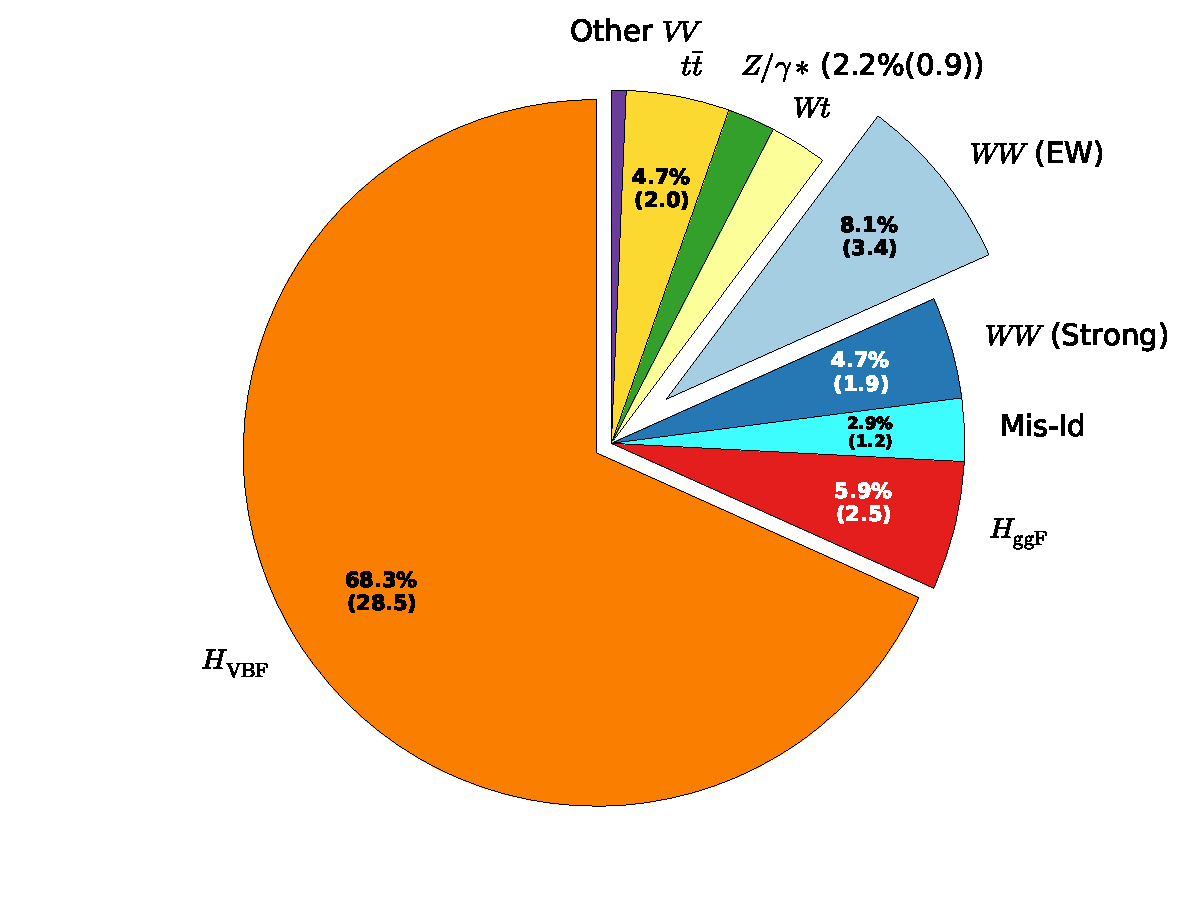
\includegraphics[width=0.49\textwidth,trim=35 0 0 0]{figures/plots/bkg-fraction-highest-bin/pie-chart-fractions-old.pdf}
        \label{fig:bkg-fractions-a}
    }
    \subfloat[Optimized EW~$WW$ training fractions] {
        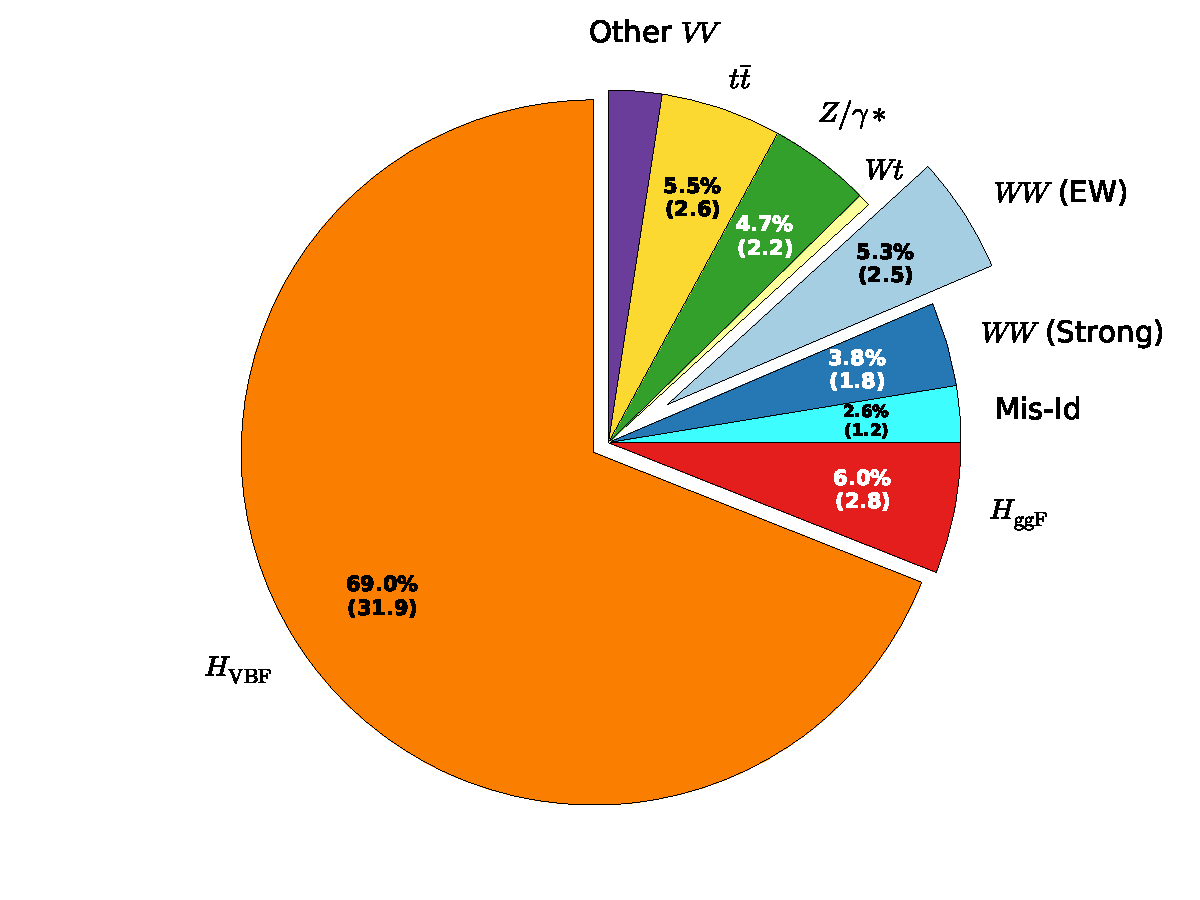
\includegraphics[width=0.49\textwidth,trim=35 0 0 0]{figures/plots/bkg-fraction-highest-bin/pie-chart-fractions-new.pdf}
        \label{fig:bkg-fractions-b}
    }
    \caption{Fraction of expected background events in the highest DNN output bin based on the validation set of a 5-fold cross-validation procedure for (a) default training fractions and (b) optimized EW~$WW$ training fraction.}
    \label{fig:bkg-fractions}
\end{figure}

% Plots made with SFUsMLKit on cedar with:
% ./plot.py -c configs/HWW/winningSubmission.cfg --trainingFolderName dropout-02-5-fold-aggressive-lr-schedule-2-fine-scan-ewww-scan-etafix/210805_9_0.12_8226149877761426764
\begin{figure}[t]
    % \subfloat[] {
    %     \newImageResizeCustom{0.47}{figures/plots/sample-fractions/sig_vs_lrate.pdf}
    % }
    % \subfloat[] {
    \newImageResizeCustom{0.6}{figures/plots/sample-fractions/sig_vs_ew_fraction_lr9.pdf}
    % }
    \caption{Significance metrics (left axis) and EW~$WW$ fraction of total background in the highest DNN output bin (right axis) for DNN models trained with different EW~$WW$ training fractions evaluated using the validation set of a 5-fold cross-validation procedure. The metric $\ZVBF$ (40 bins) is calculated as described in \cref{subsec:performance-metrics} and using 40 equidistant histogram bins. The metric $\ZVBF$ (var. bins) is calculated similarly but using a rebinned histogram according to the procedure outlined in \cref{subsec:performance-metrics}. The metric $\ZVBFunc$ (var. bins), other than the other ones, consider rough estimates of systematic uncertainties for the different processes, also using a rebinned histogram. The assumed uncertainties are shown in \cref{tab:rough-uncertainties}.}
    \label{fig:ew-fraction-scan}
\end{figure}


\FloatBarrier
\chapter{Auxiliary Material for \HWW Analysis}
This section provides various material related to the \HWW analysis presented in \cref{chap:hww} of this thesis.

\clearpage
\FloatBarrier
\section[Distributions of the VBF DNN input variables]{Distributions of the VBF DNN input variables with selections on the DNN}
\label{app:dnn:input-vars}
To show the effect of the DNN on the DNN input variables, \cref{app:fig:dnn-inputs-vbf-top1,app:fig:dnn-inputs-vbf-top2,app:fig:dnn-inputs-vbf-top3,app:fig:dnn-inputs-hwwdecay,app:fig:dnn-inputs-top-sup} show distributions of the DNN input variables with different selections on the DNN output.
This nicely shows the kinematics and topologies the DNN selects to define regions pure in the VBF signal.

    \begin{figure}[ht]
        \centering
        \subfloat[$\mjj$]{
            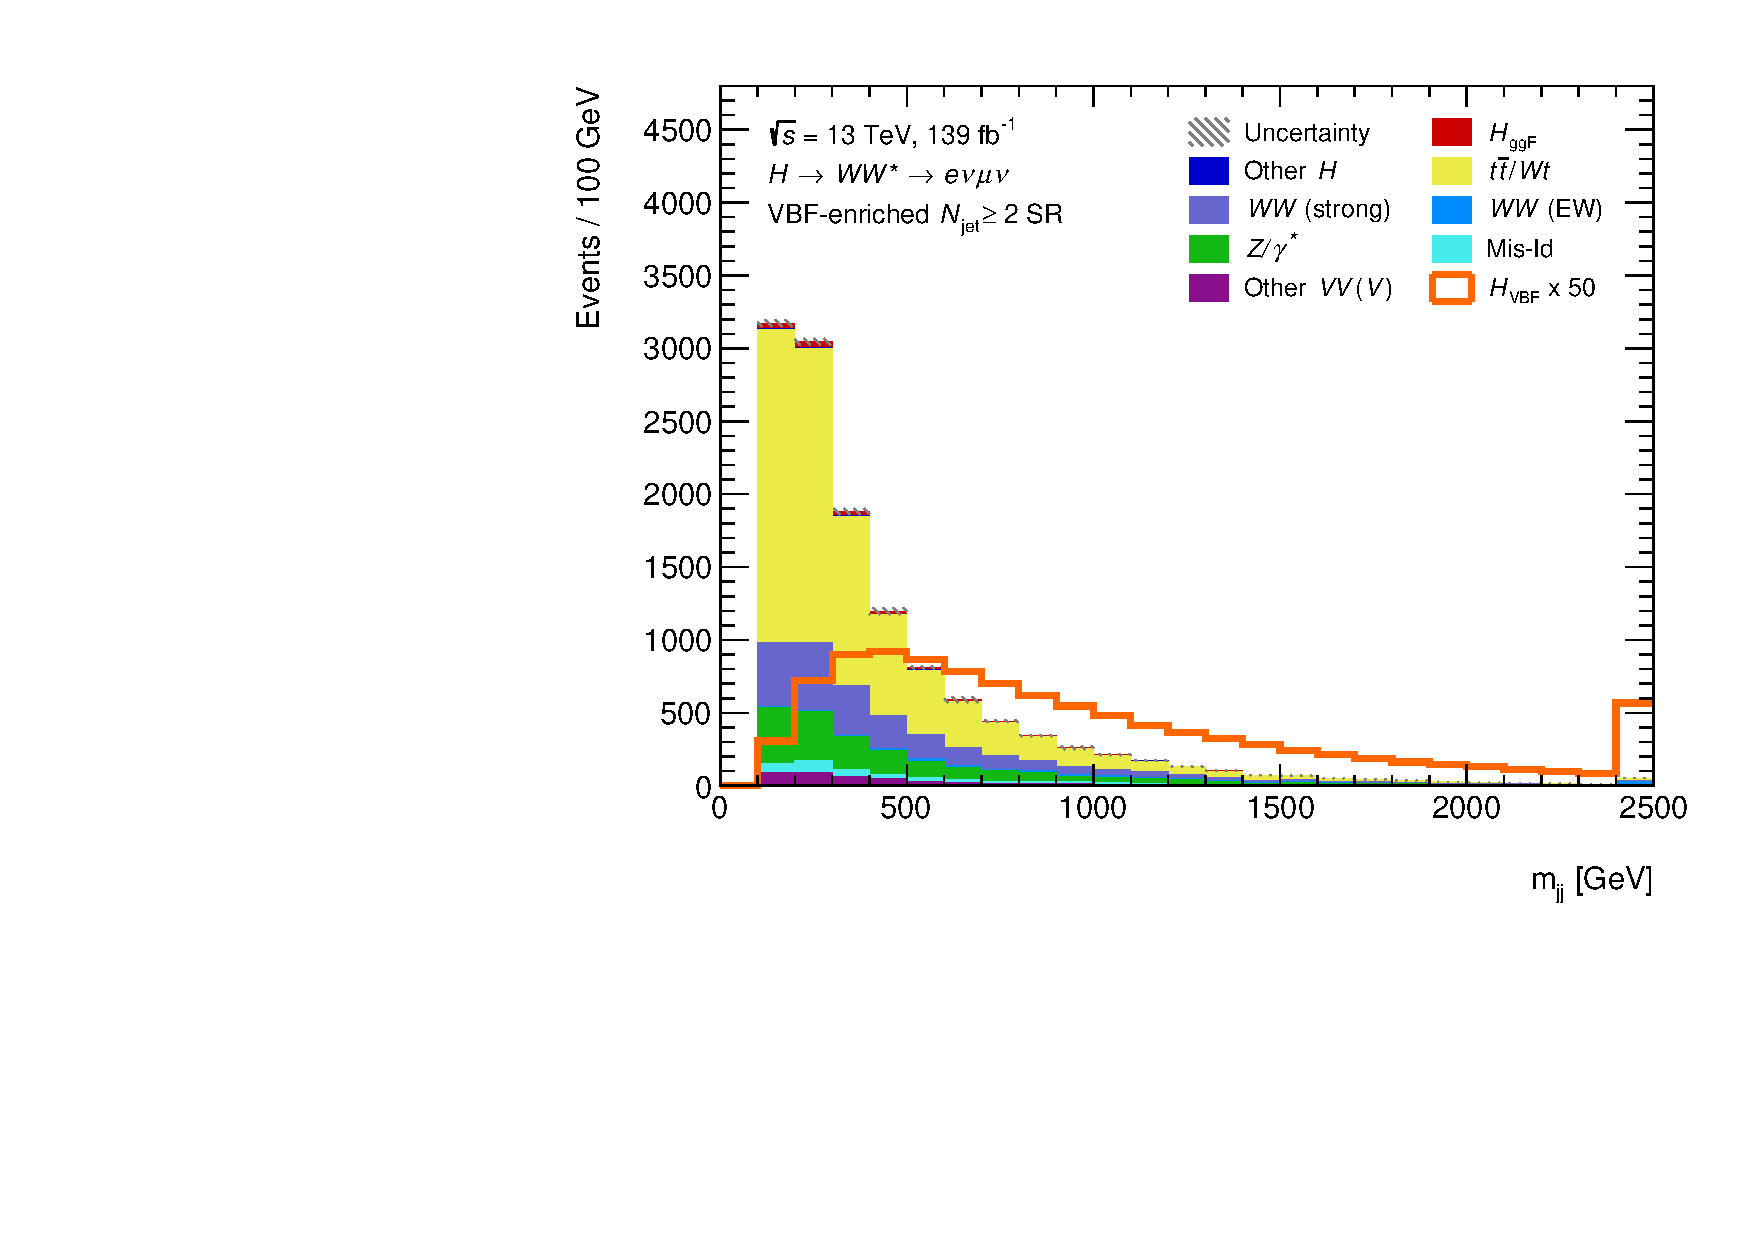
\includegraphics[width=0.32\textwidth]{figures/hww/dnn/blinded/run2-emme-CutVBF_SR-Mjj-lin.pdf} \hfill
            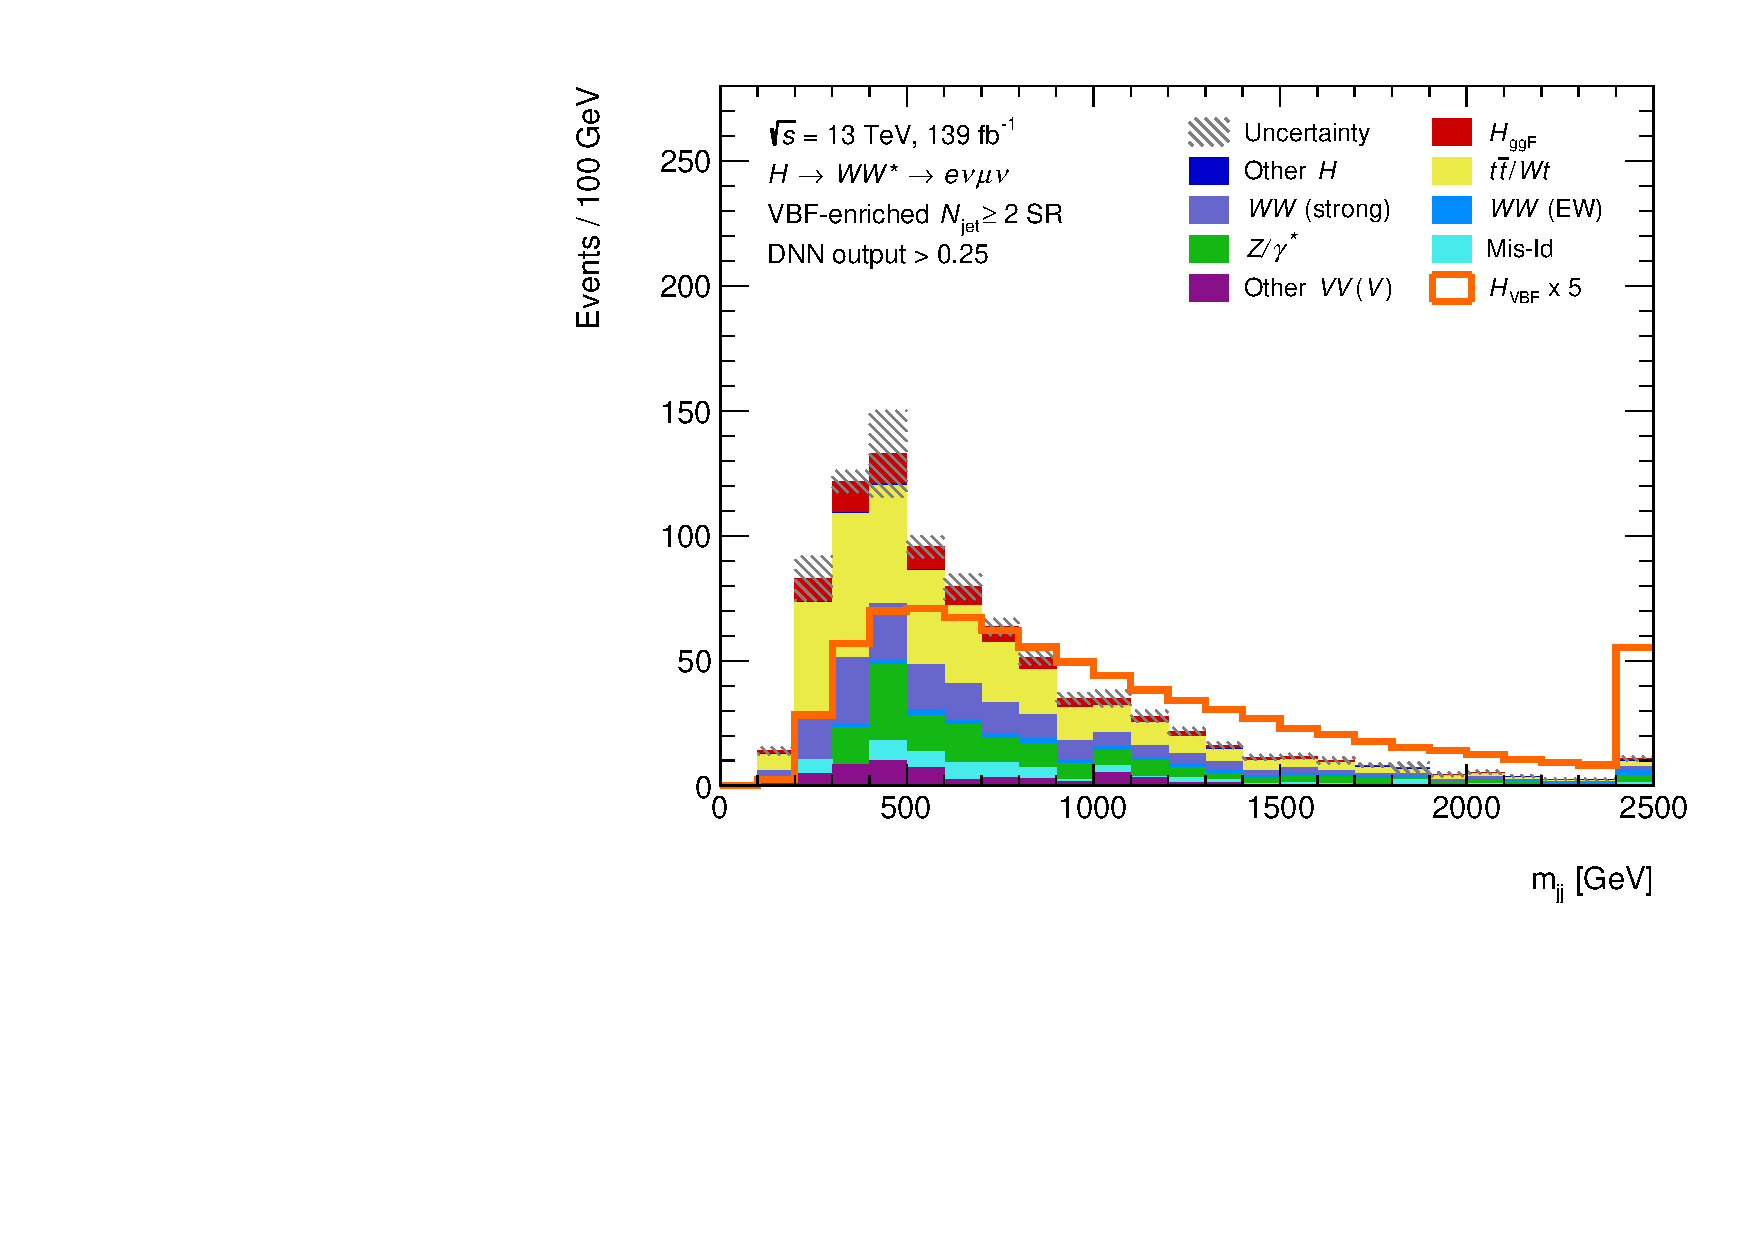
\includegraphics[width=0.32\textwidth]{figures/hww/dnn/blinded/run2-emme-CutVBFSR_DNN25-Mjj-lin.pdf} \hfill
            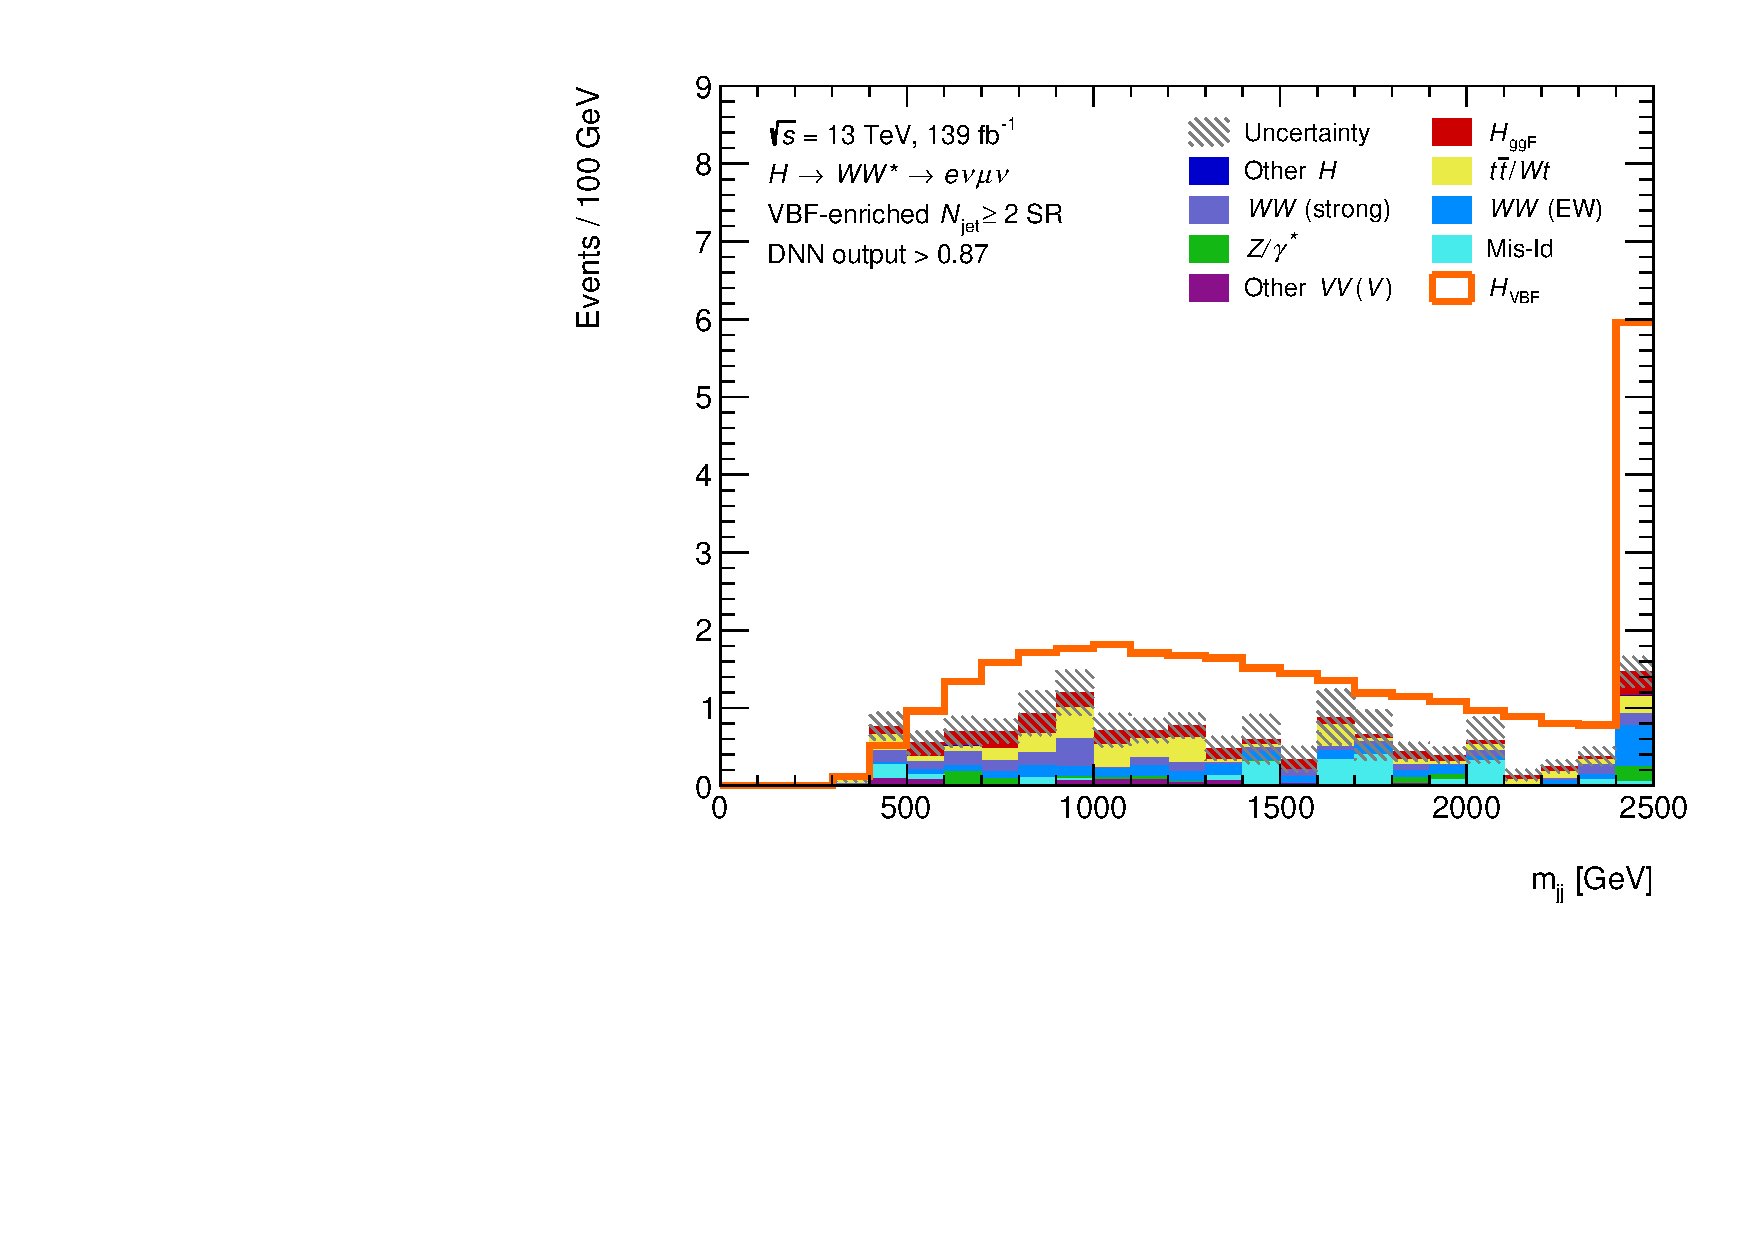
\includegraphics[width=0.32\textwidth]{figures/hww/dnn/blinded/run2-emme-CutVBFSR_DNN87-Mjj-lin.pdf}
        } \\
        \subfloat[$\dyjj$]{
            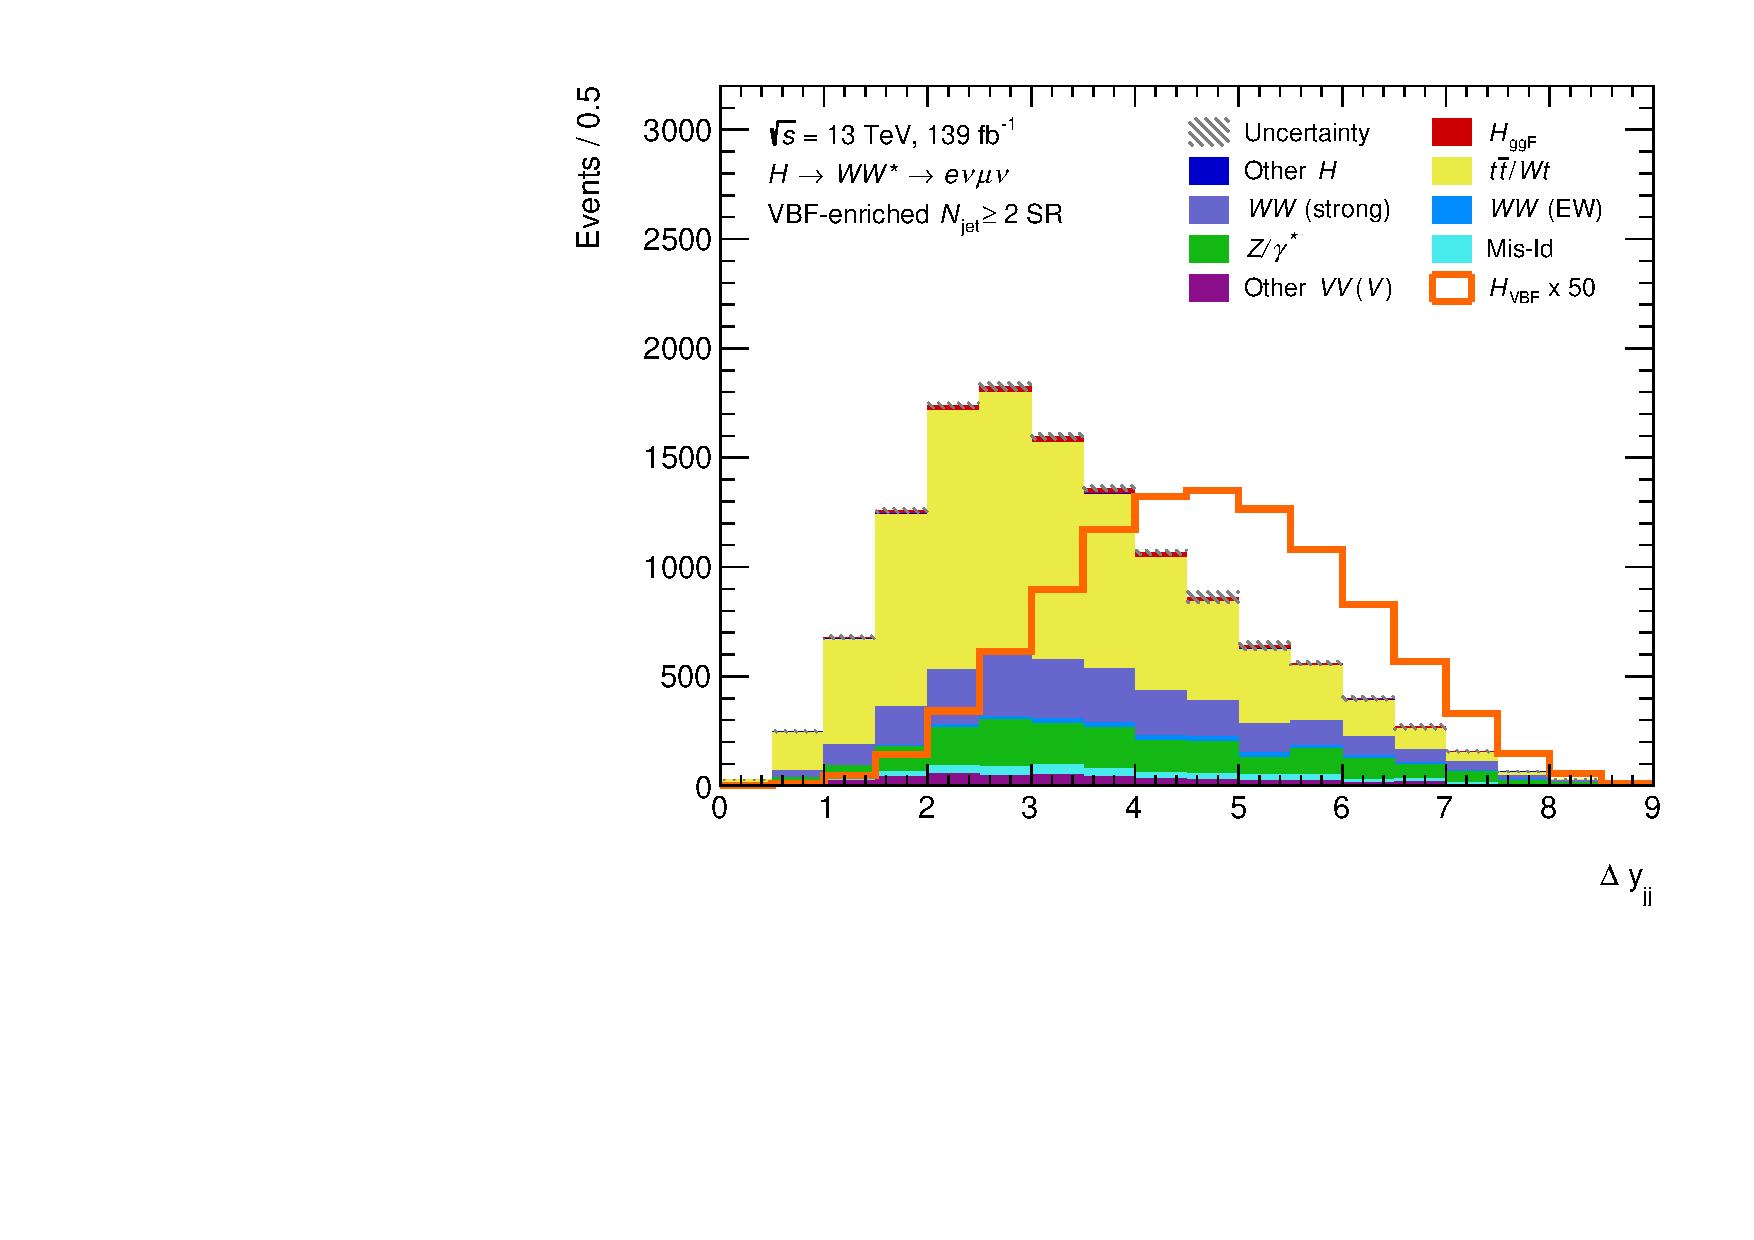
\includegraphics[width=0.32\textwidth]{figures/hww/dnn/blinded/run2-emme-CutVBF_SR-DYjj-lin.pdf} \hfill
            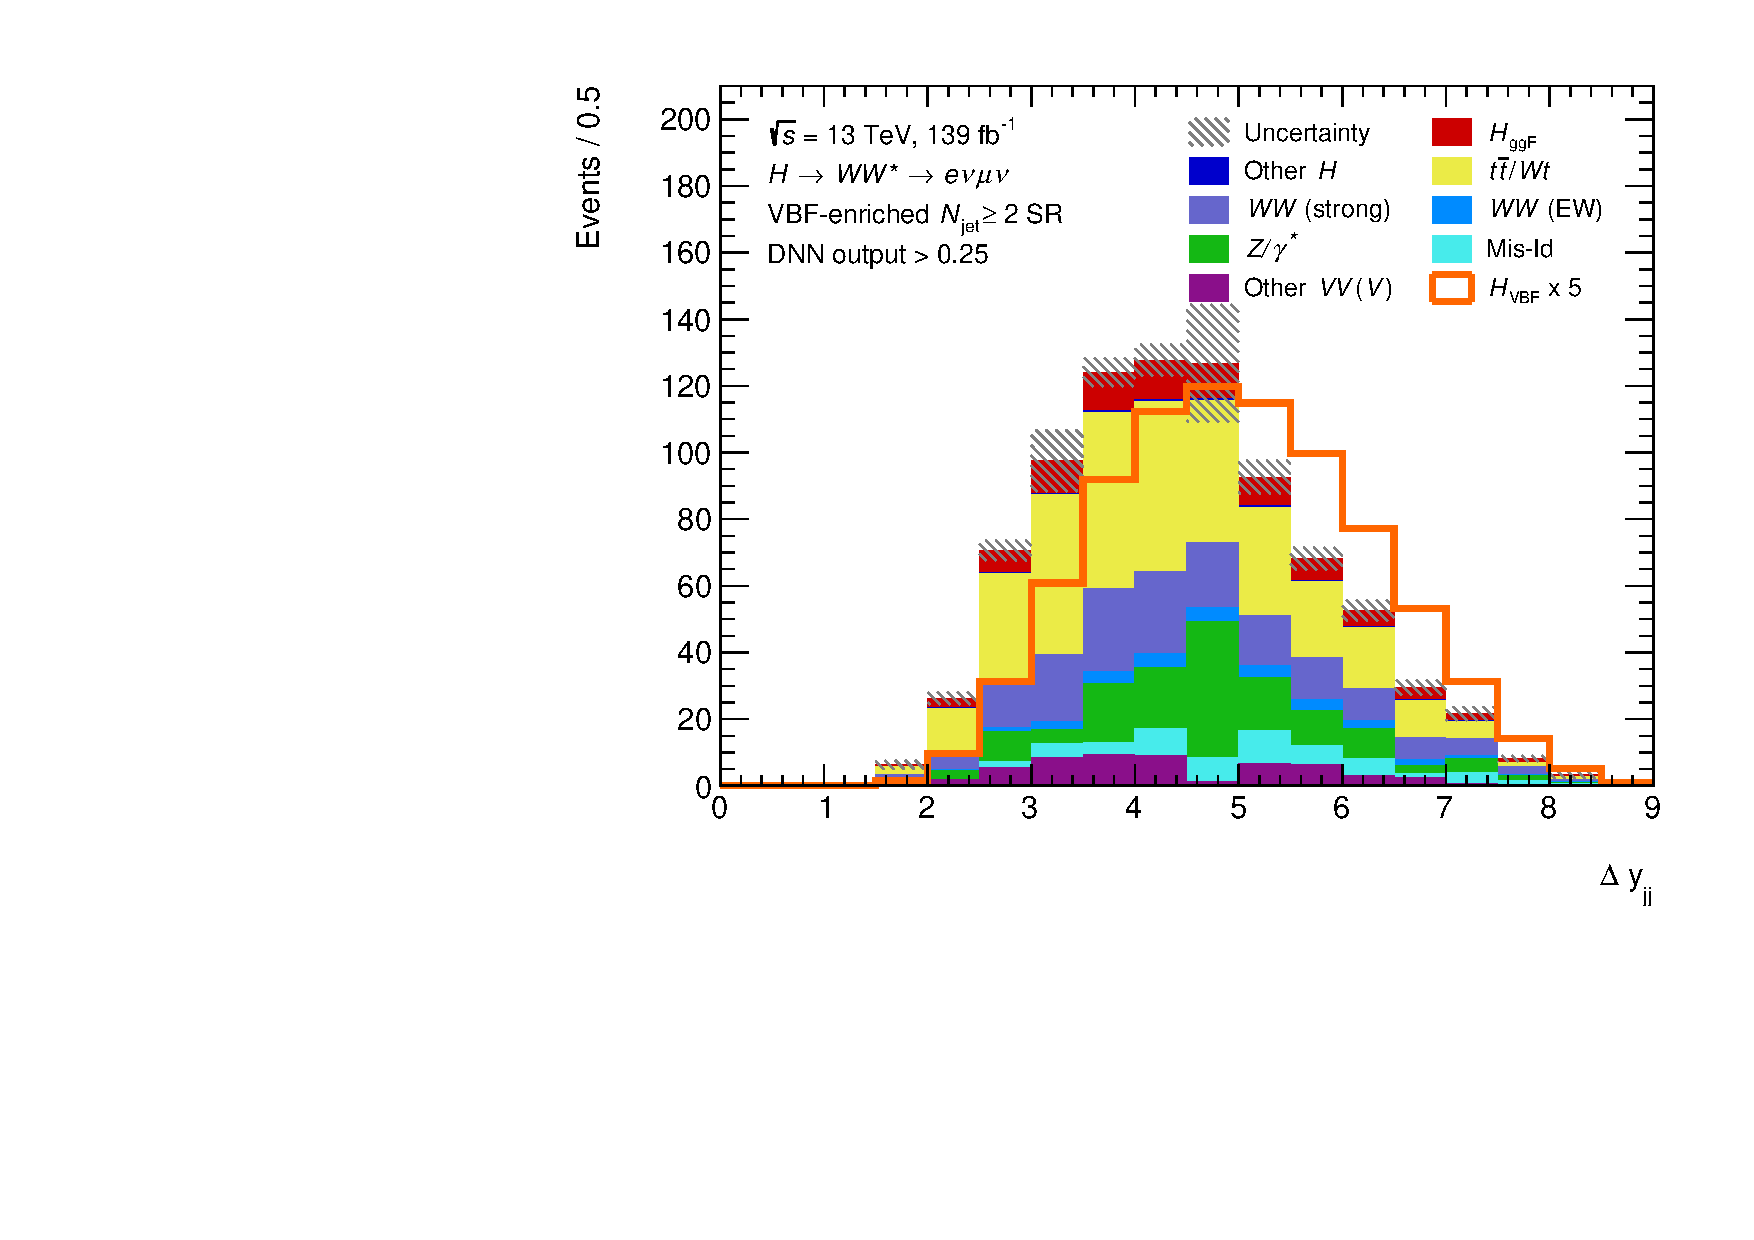
\includegraphics[width=0.32\textwidth]{figures/hww/dnn/blinded/run2-emme-CutVBFSR_DNN25-DYjj-lin.pdf} \hfill
            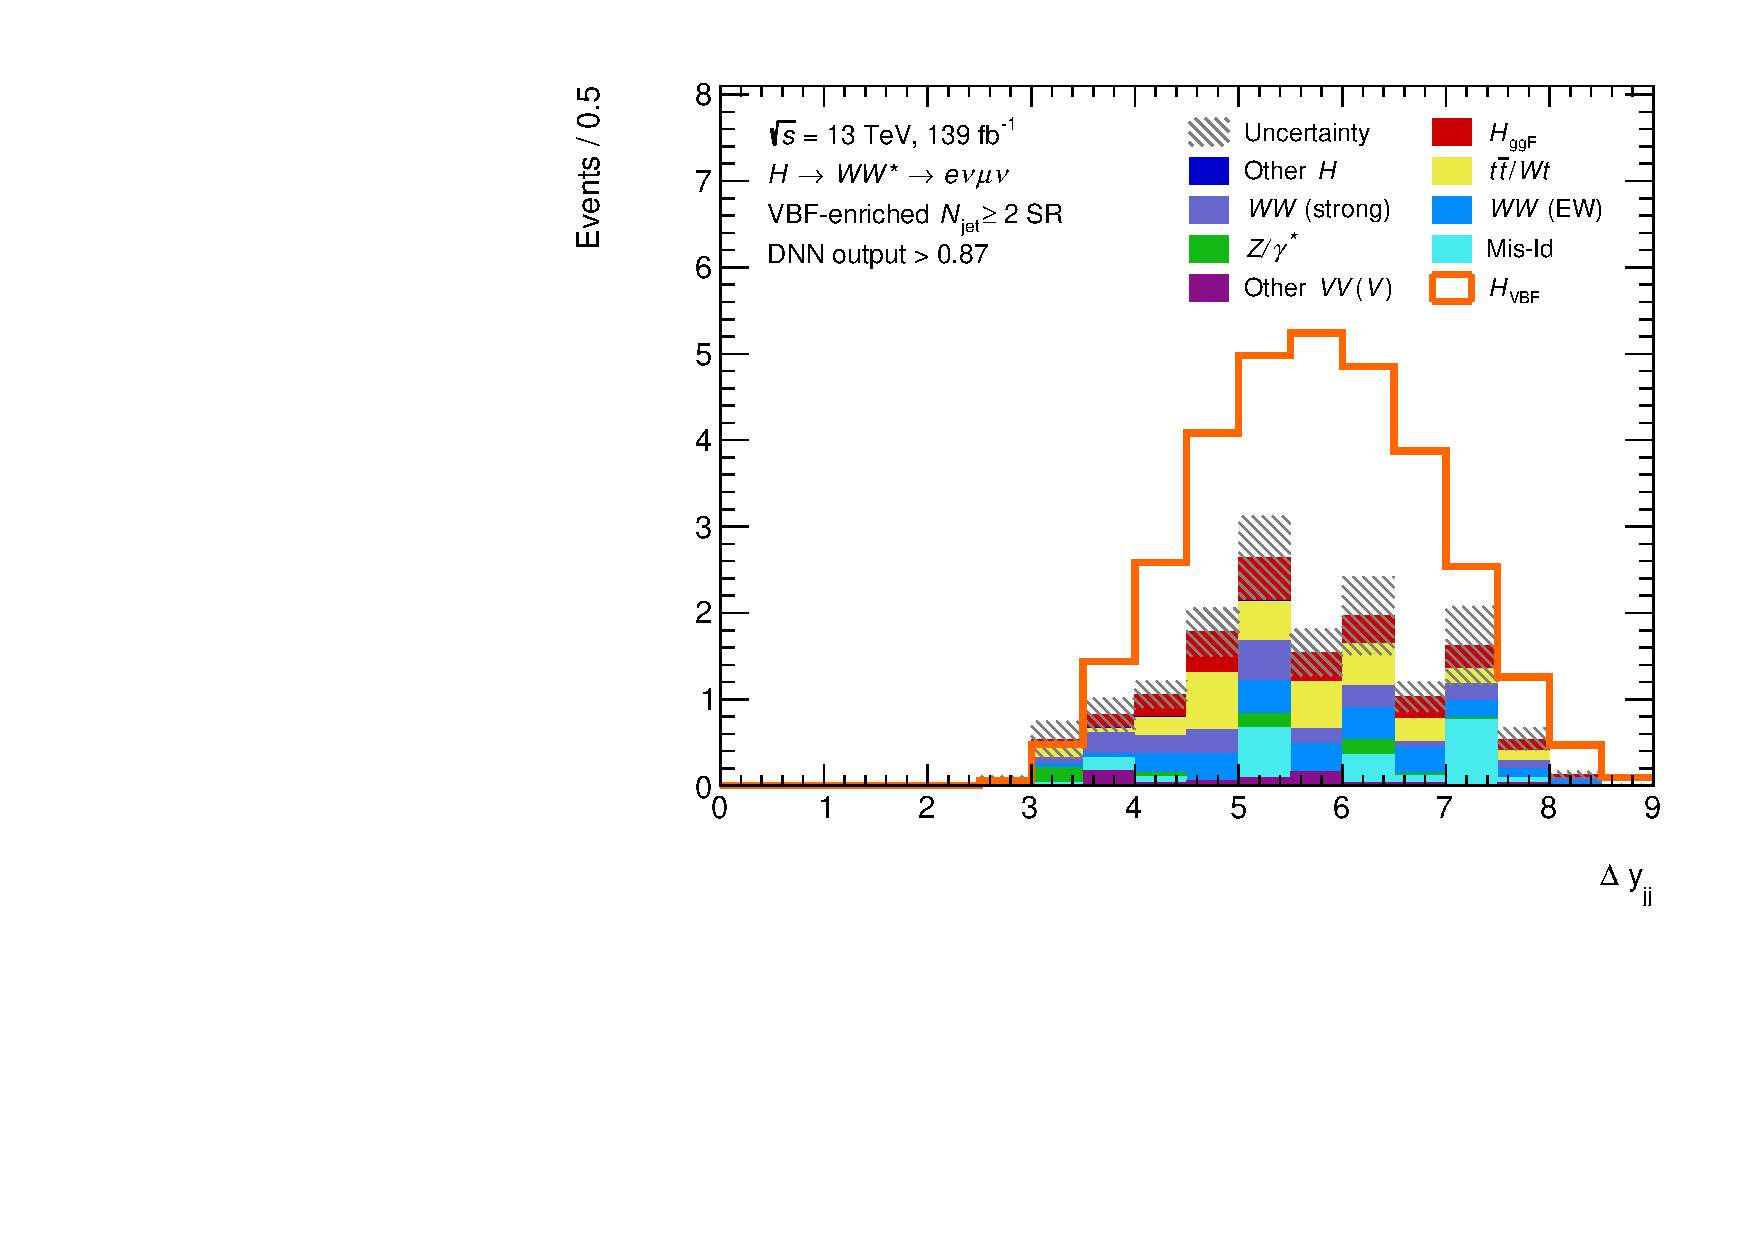
\includegraphics[width=0.32\textwidth]{figures/hww/dnn/blinded/run2-emme-CutVBFSR_DNN87-DYjj-lin.pdf}
        } \\
        \subfloat[$\lepetacent$]{
            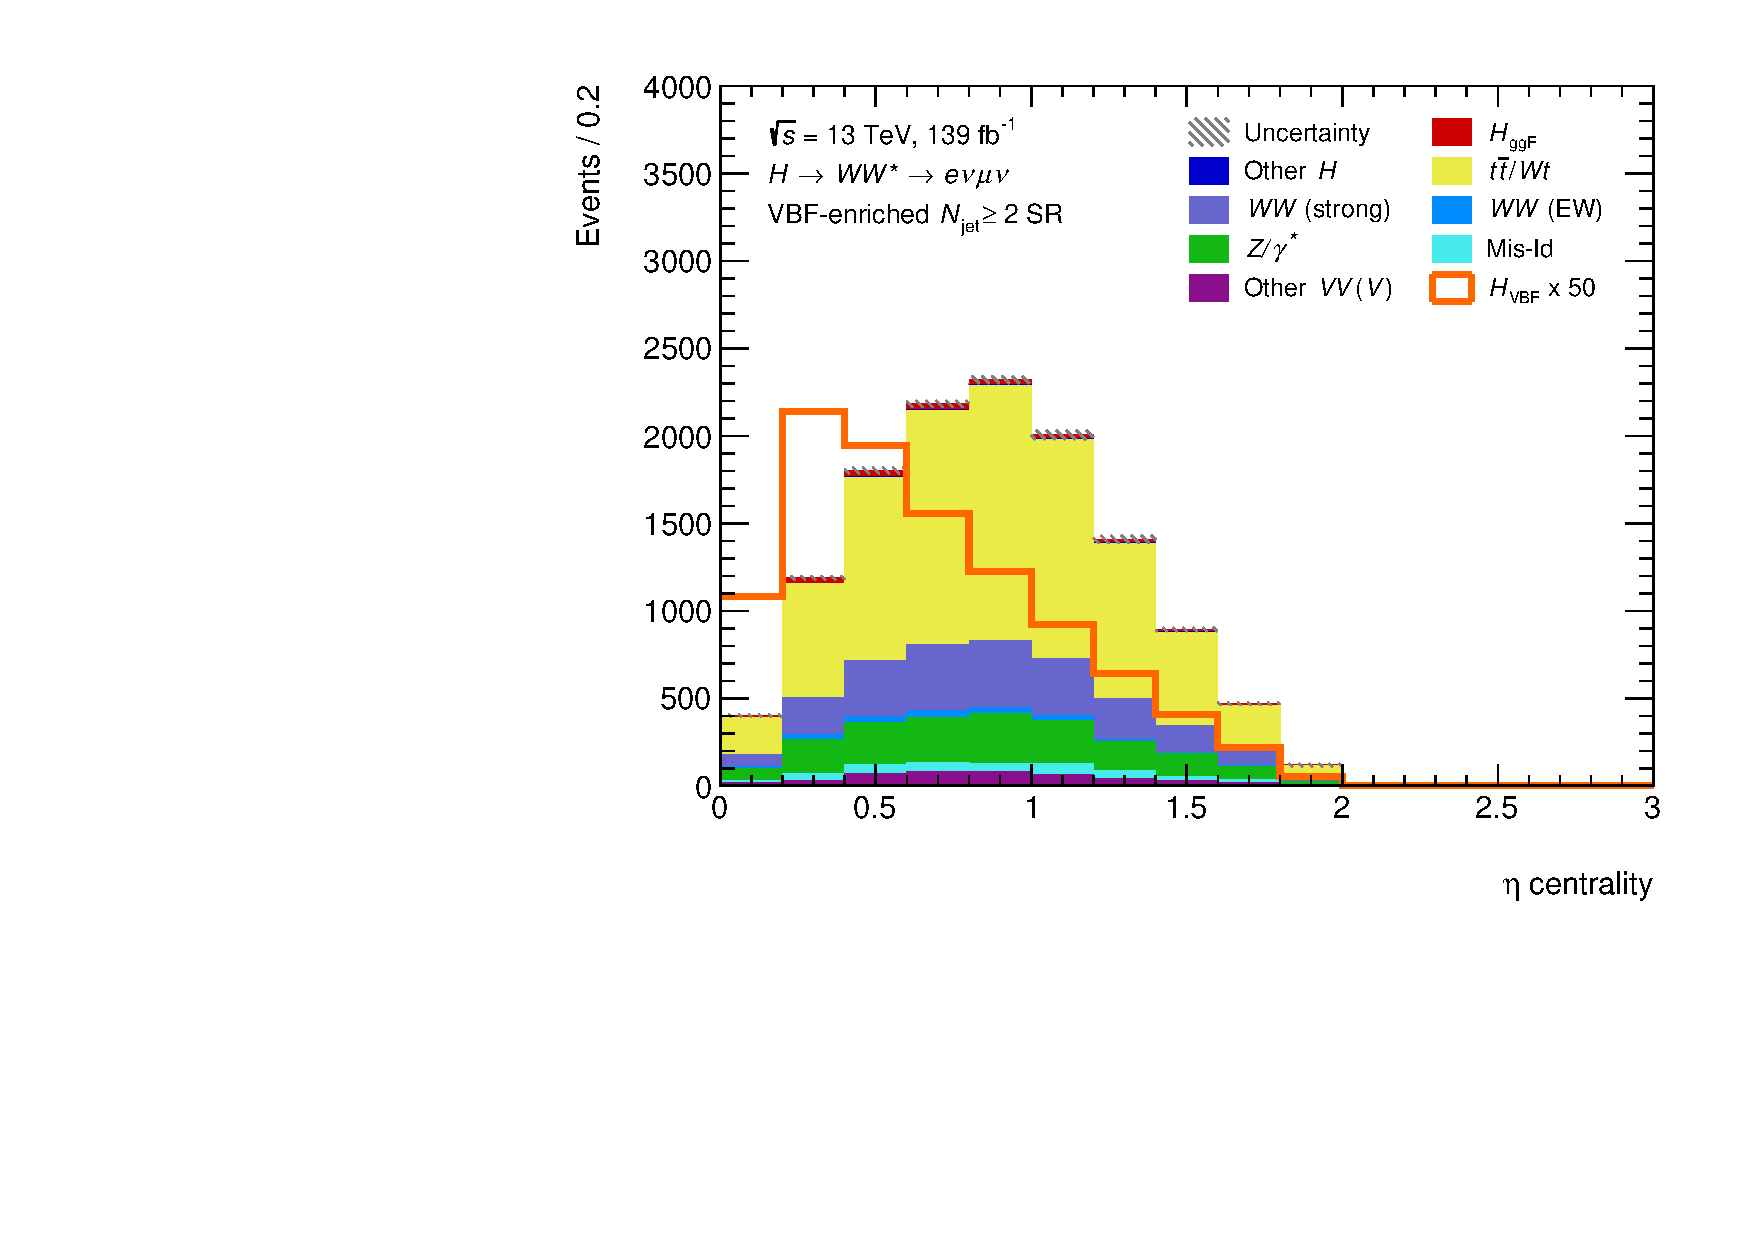
\includegraphics[width=0.32\textwidth]{figures/hww/dnn/blinded/run2-emme-CutVBF_SR-contOLV-lin.pdf} \hfill
            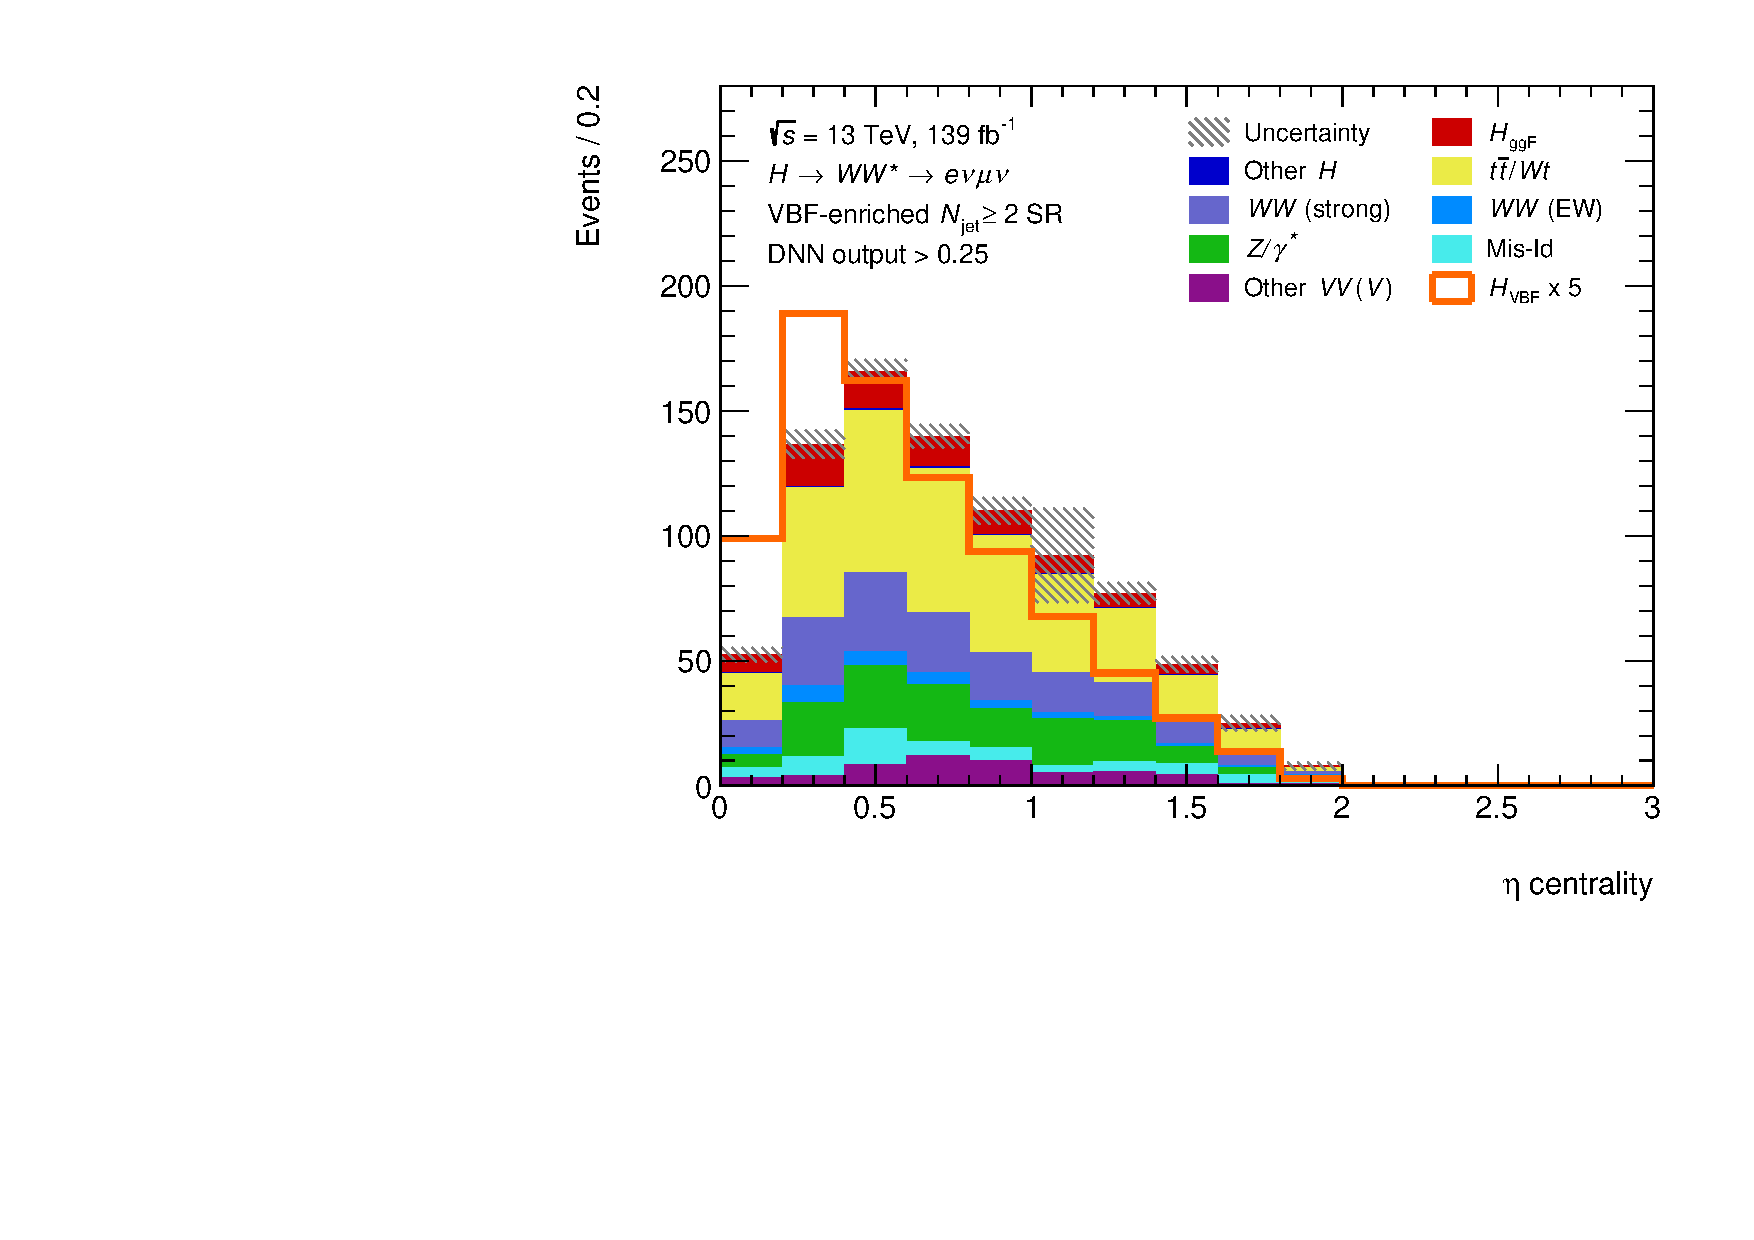
\includegraphics[width=0.32\textwidth]{figures/hww/dnn/blinded/run2-emme-CutVBFSR_DNN25-contOLV-lin.pdf} \hfill
            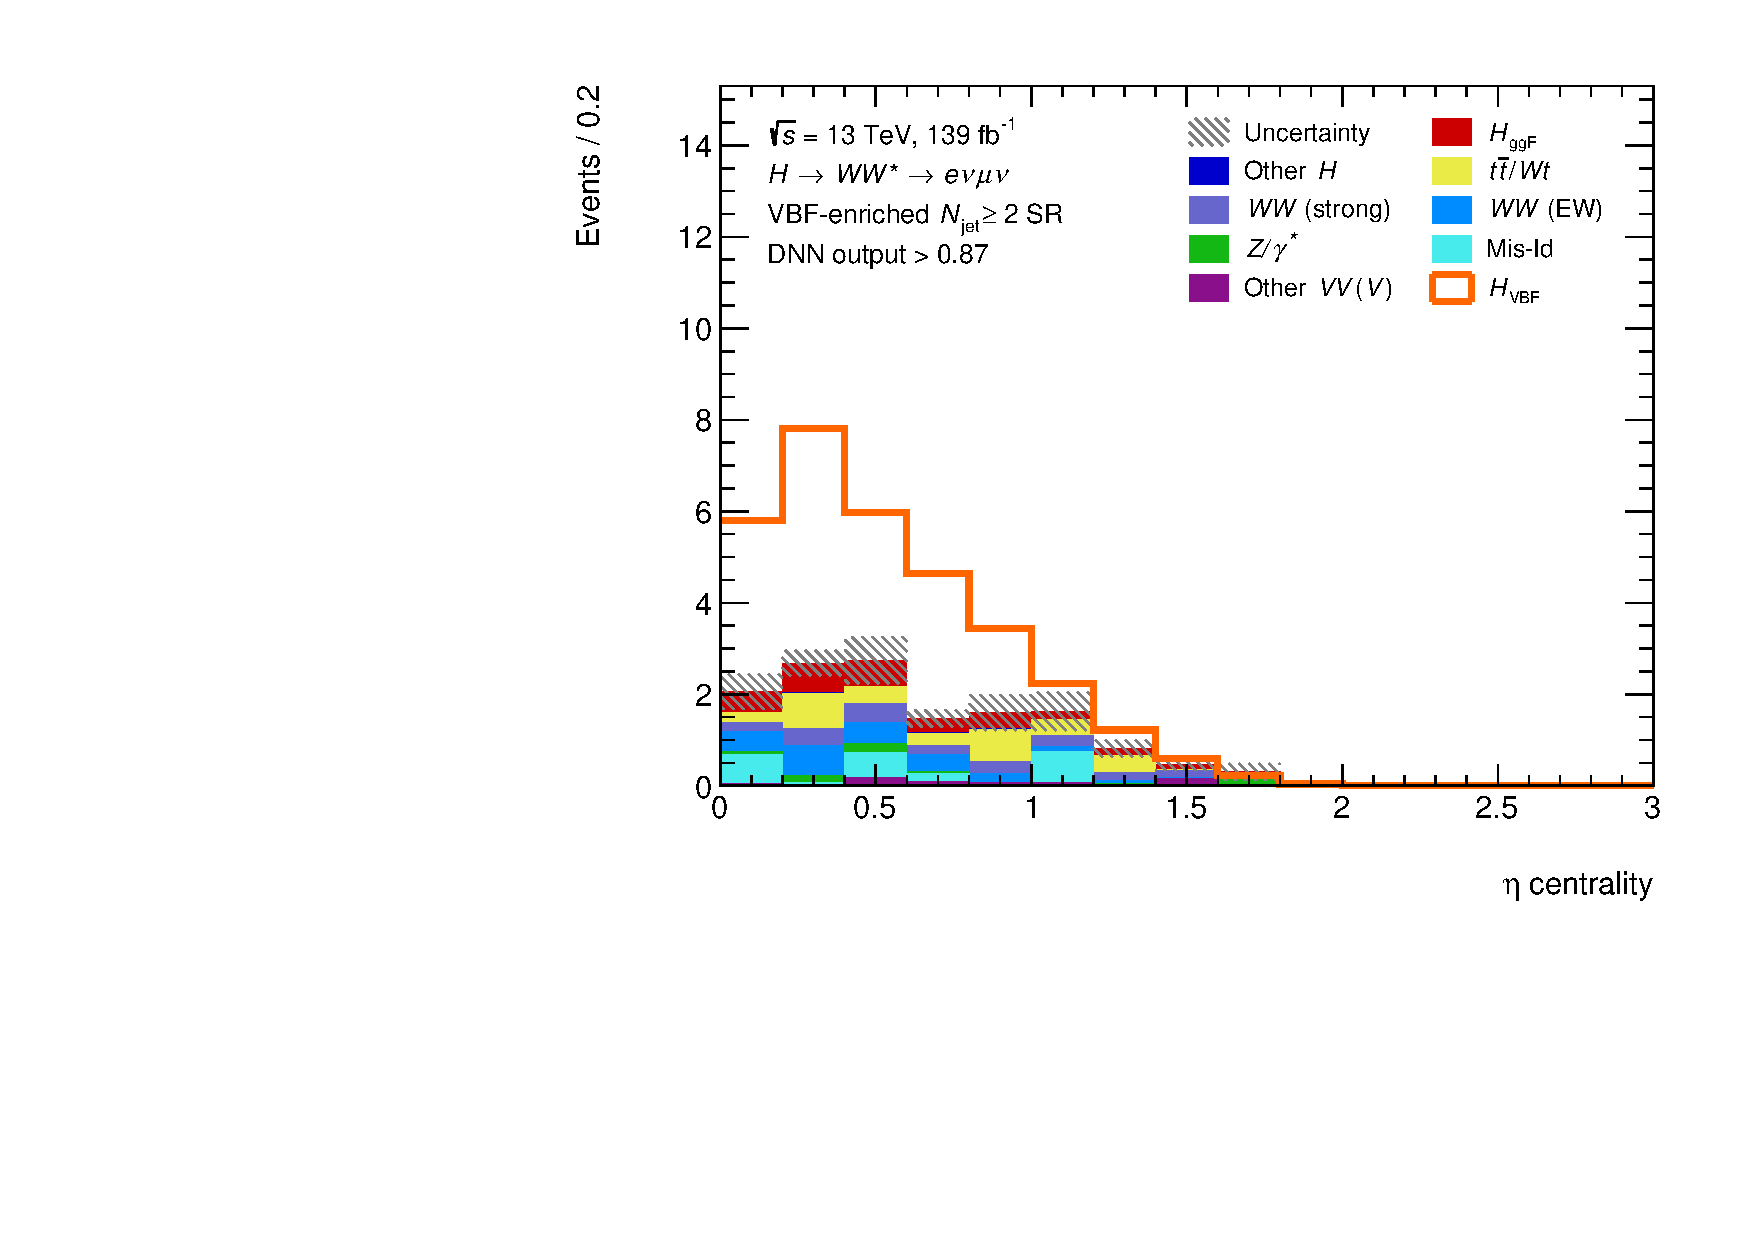
\includegraphics[width=0.32\textwidth]{figures/hww/dnn/blinded/run2-emme-CutVBFSR_DNN87-contOLV-lin.pdf}
        } \\
        {\caption[Distributions of $\mjj$, $\dyjj$, $\lepetacent$ in the VBF \TwoJet signal region.]{Distributions of $\mjj$, $\dyjj$, $\lepetacent$ in the VBF \TwoJet signal region.
            Each row corresponds to one variable with different selections made on the DNN output as indicated in the figure. The solid orange line shows the expected VBF signal scaled by a factor of (left) 50, (center) 5, and (right) without any scaling.
            \label{app:fig:dnn-inputs-vbf-top1} }}
    \end{figure}


    \begin{figure}[h]
        \centering
        \subfloat[$\mlonejtwo$]{
            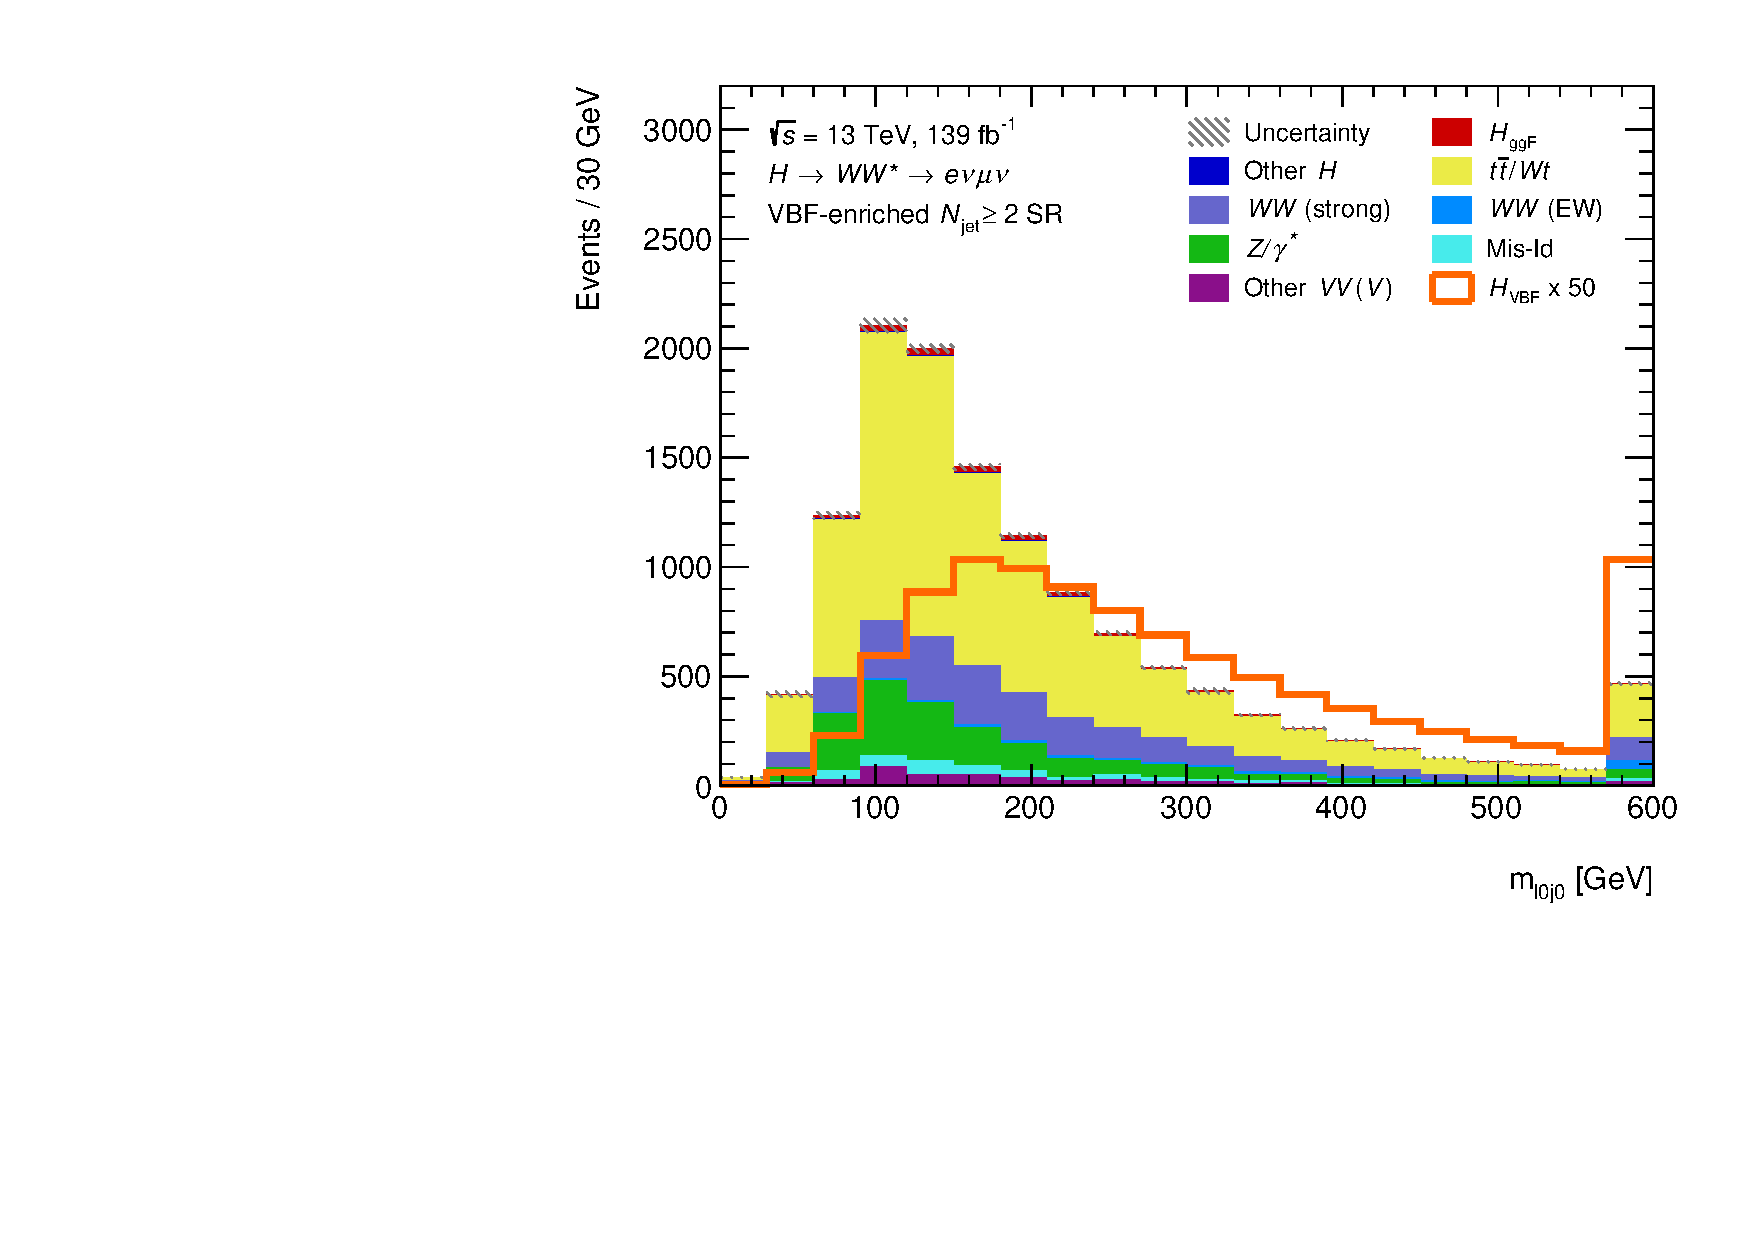
\includegraphics[width=0.32\textwidth]{figures/hww/dnn/blinded/run2-emme-CutVBF_SR-Ml0j0-lin.pdf} \hfill
            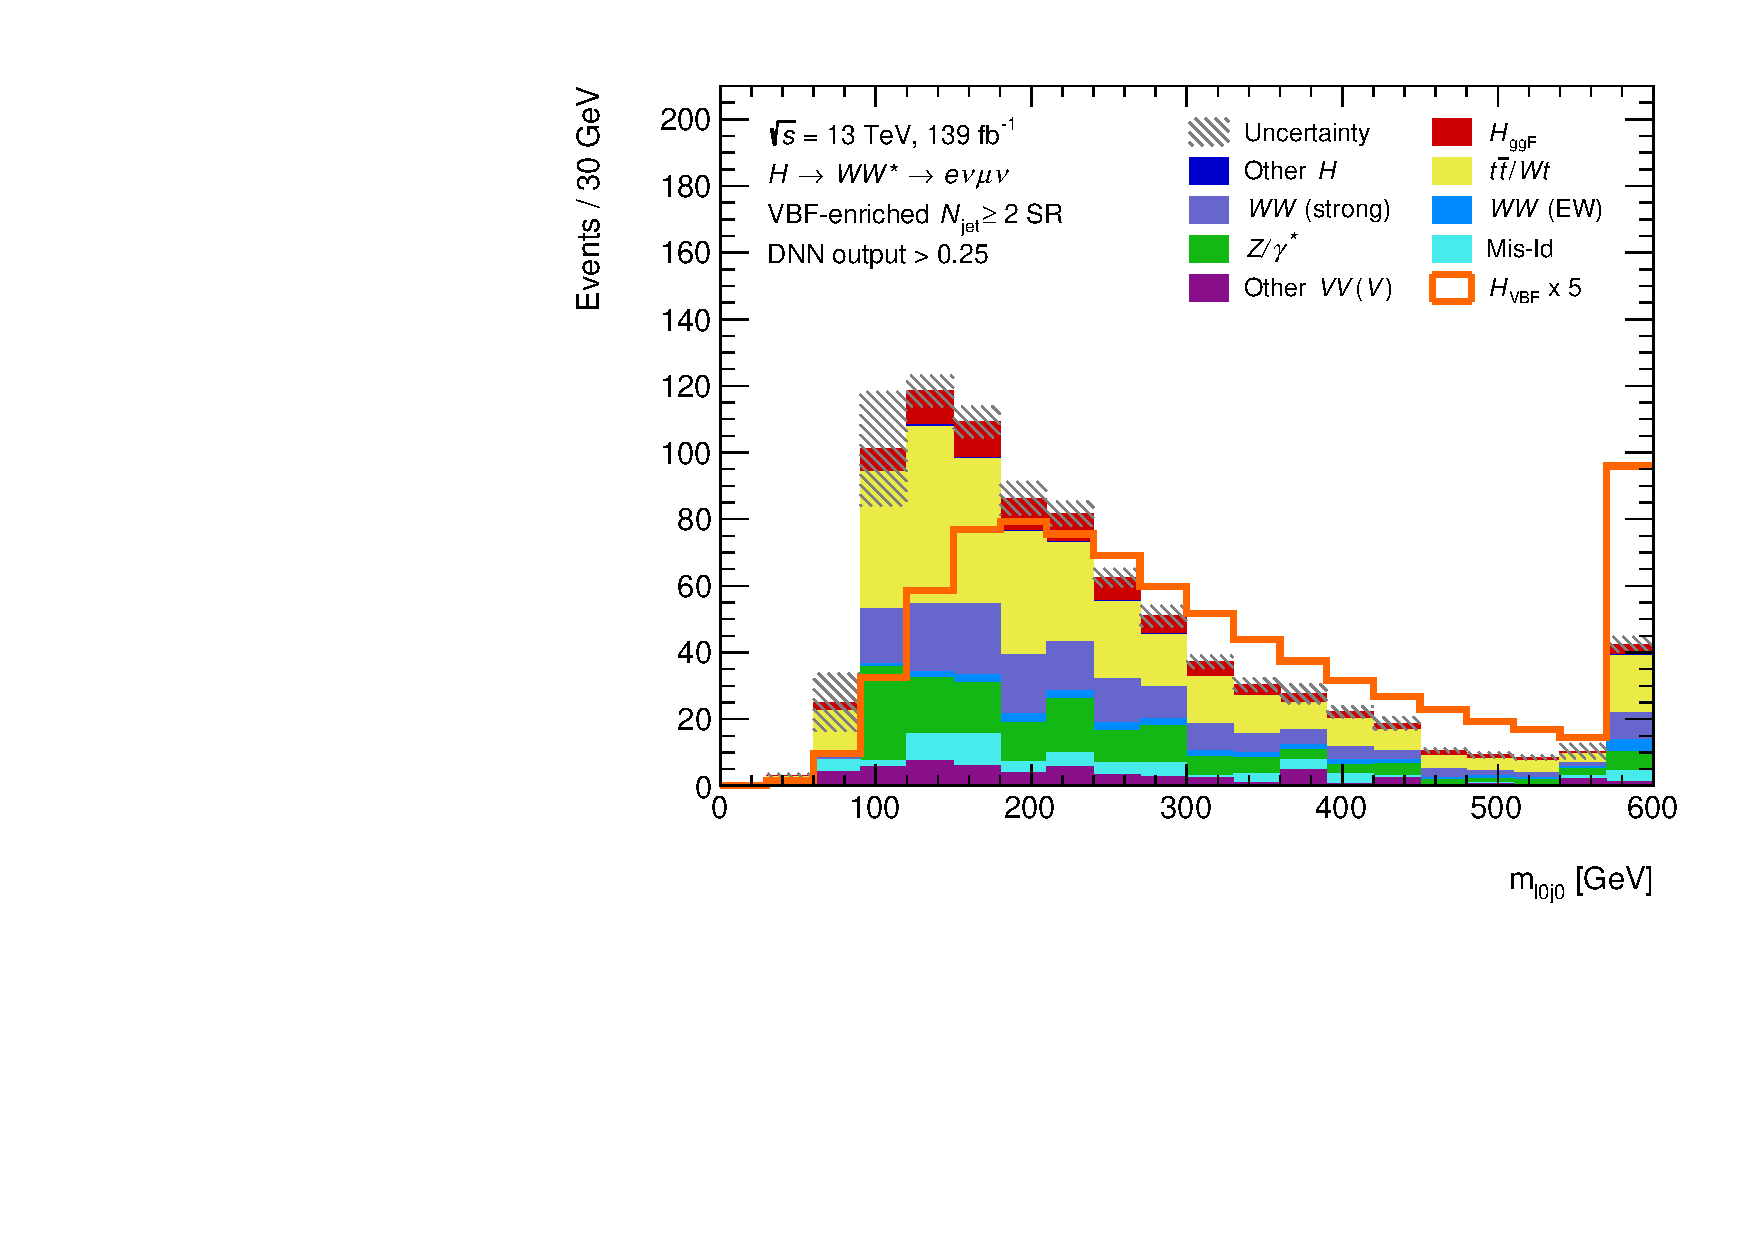
\includegraphics[width=0.32\textwidth]{figures/hww/dnn/blinded/run2-emme-CutVBFSR_DNN25-Ml0j0-lin.pdf} \hfill
            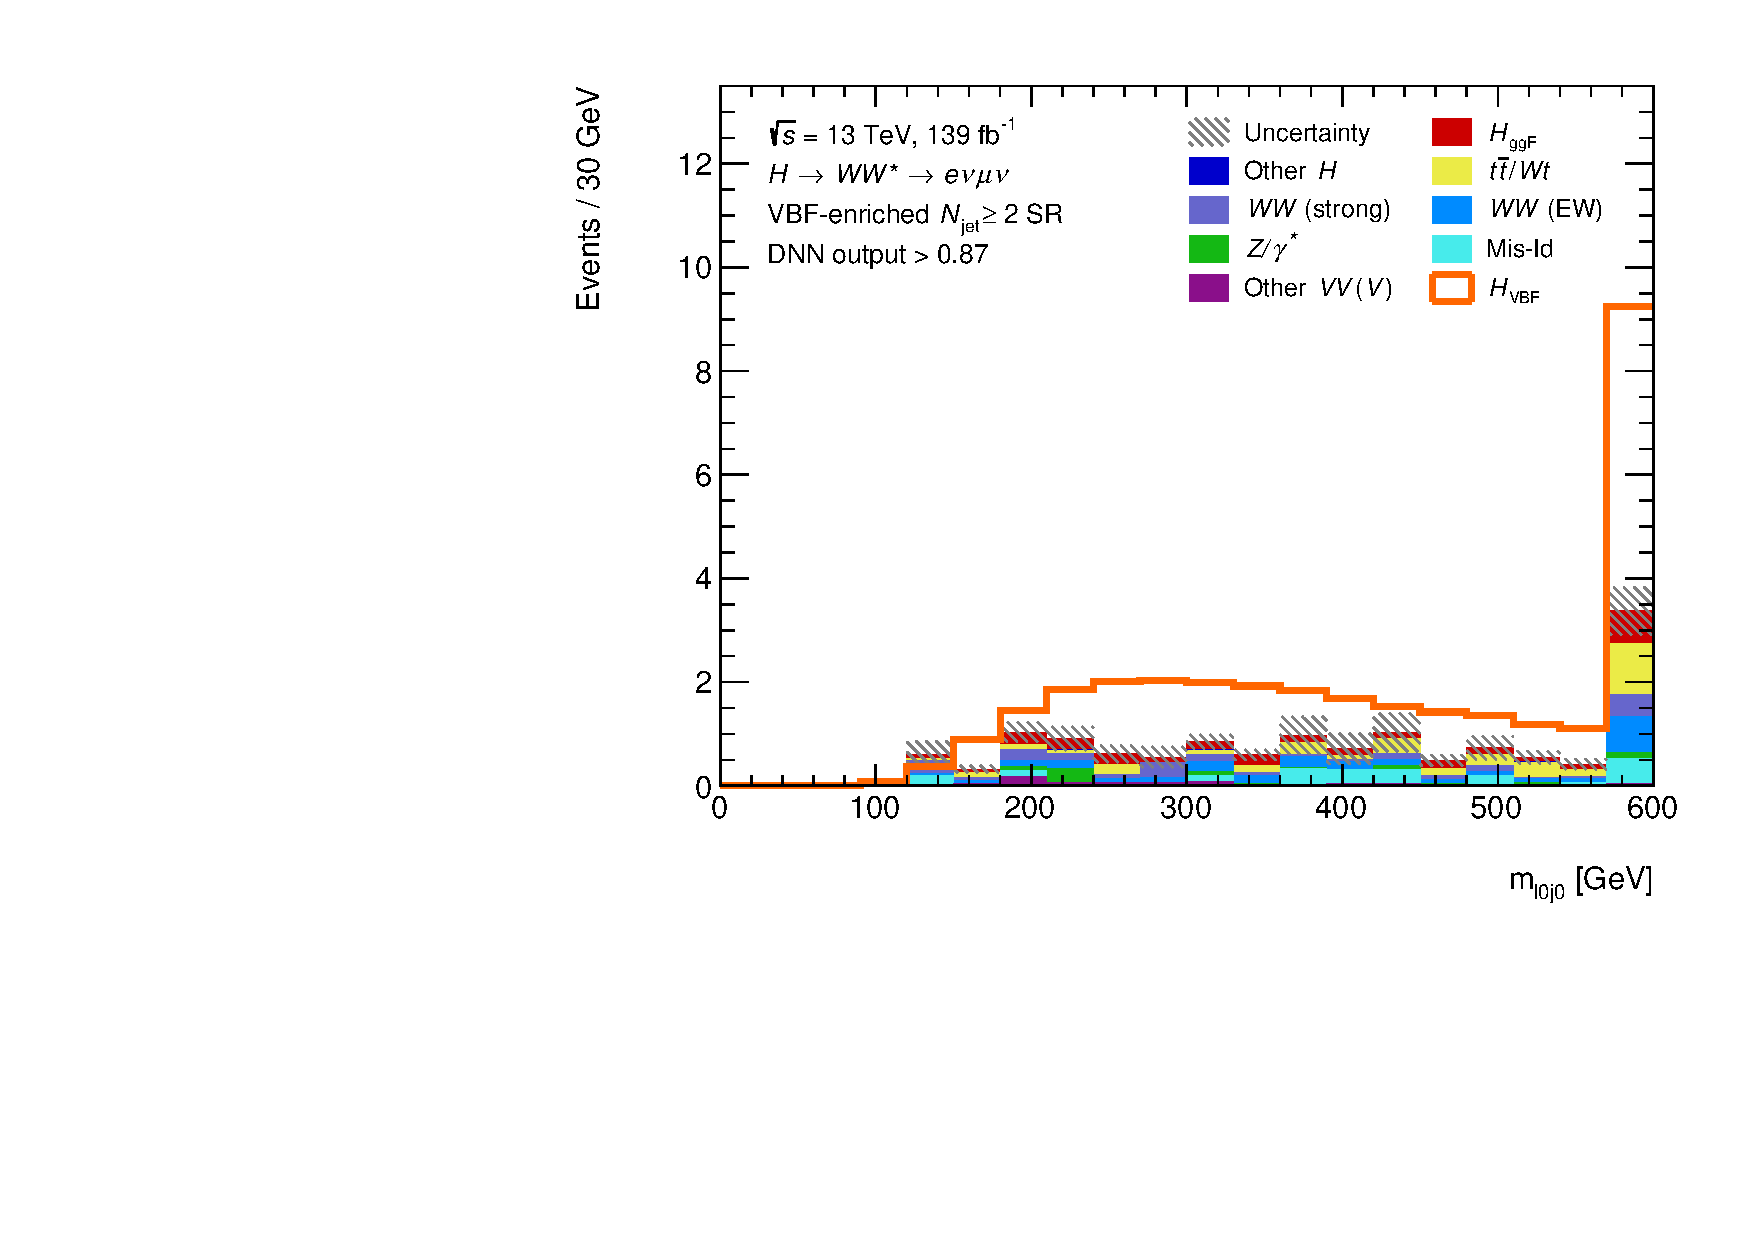
\includegraphics[width=0.32\textwidth]{figures/hww/dnn/blinded/run2-emme-CutVBFSR_DNN87-Ml0j0-lin.pdf}
        } \\
        \subfloat[$\mltwojone$]{
            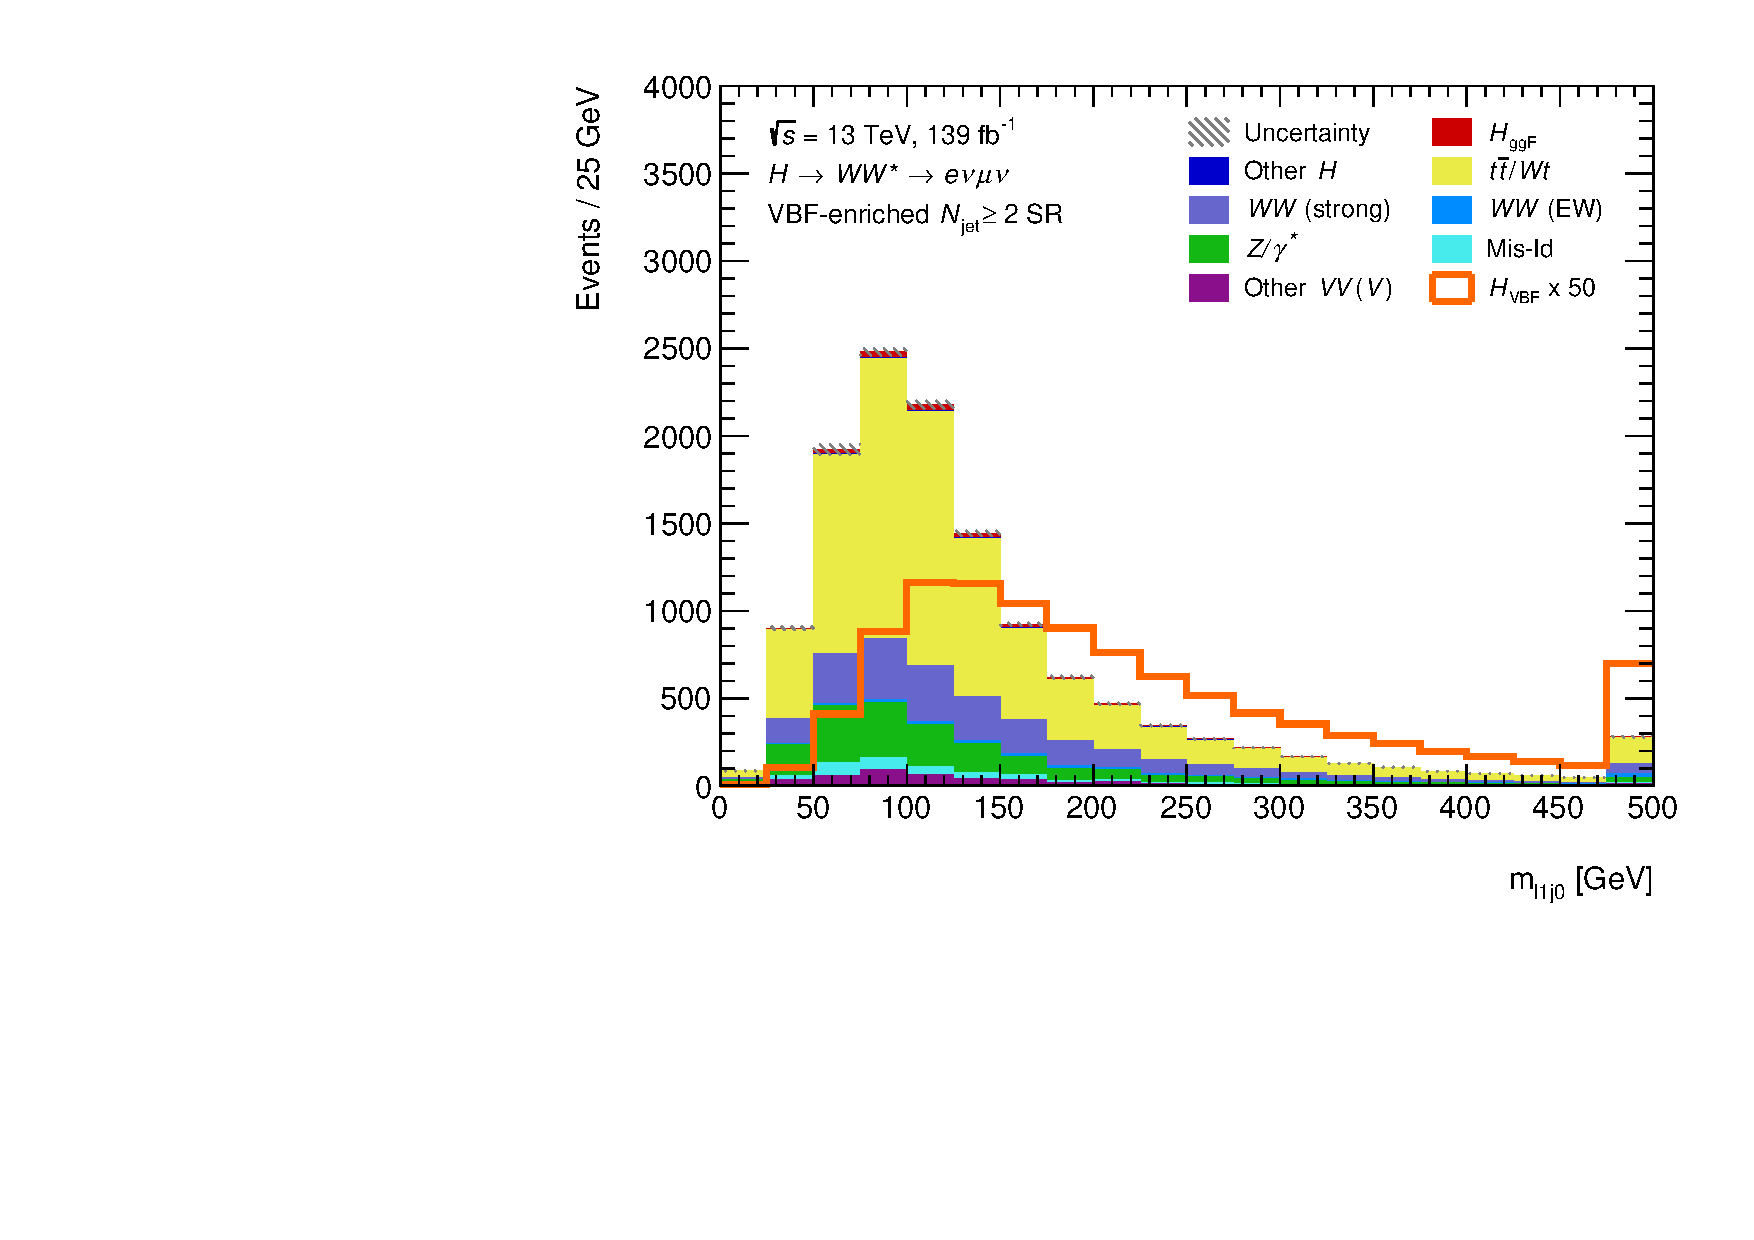
\includegraphics[width=0.32\textwidth]{figures/hww/dnn/blinded/run2-emme-CutVBF_SR-Ml1j0-lin.pdf} \hfill
            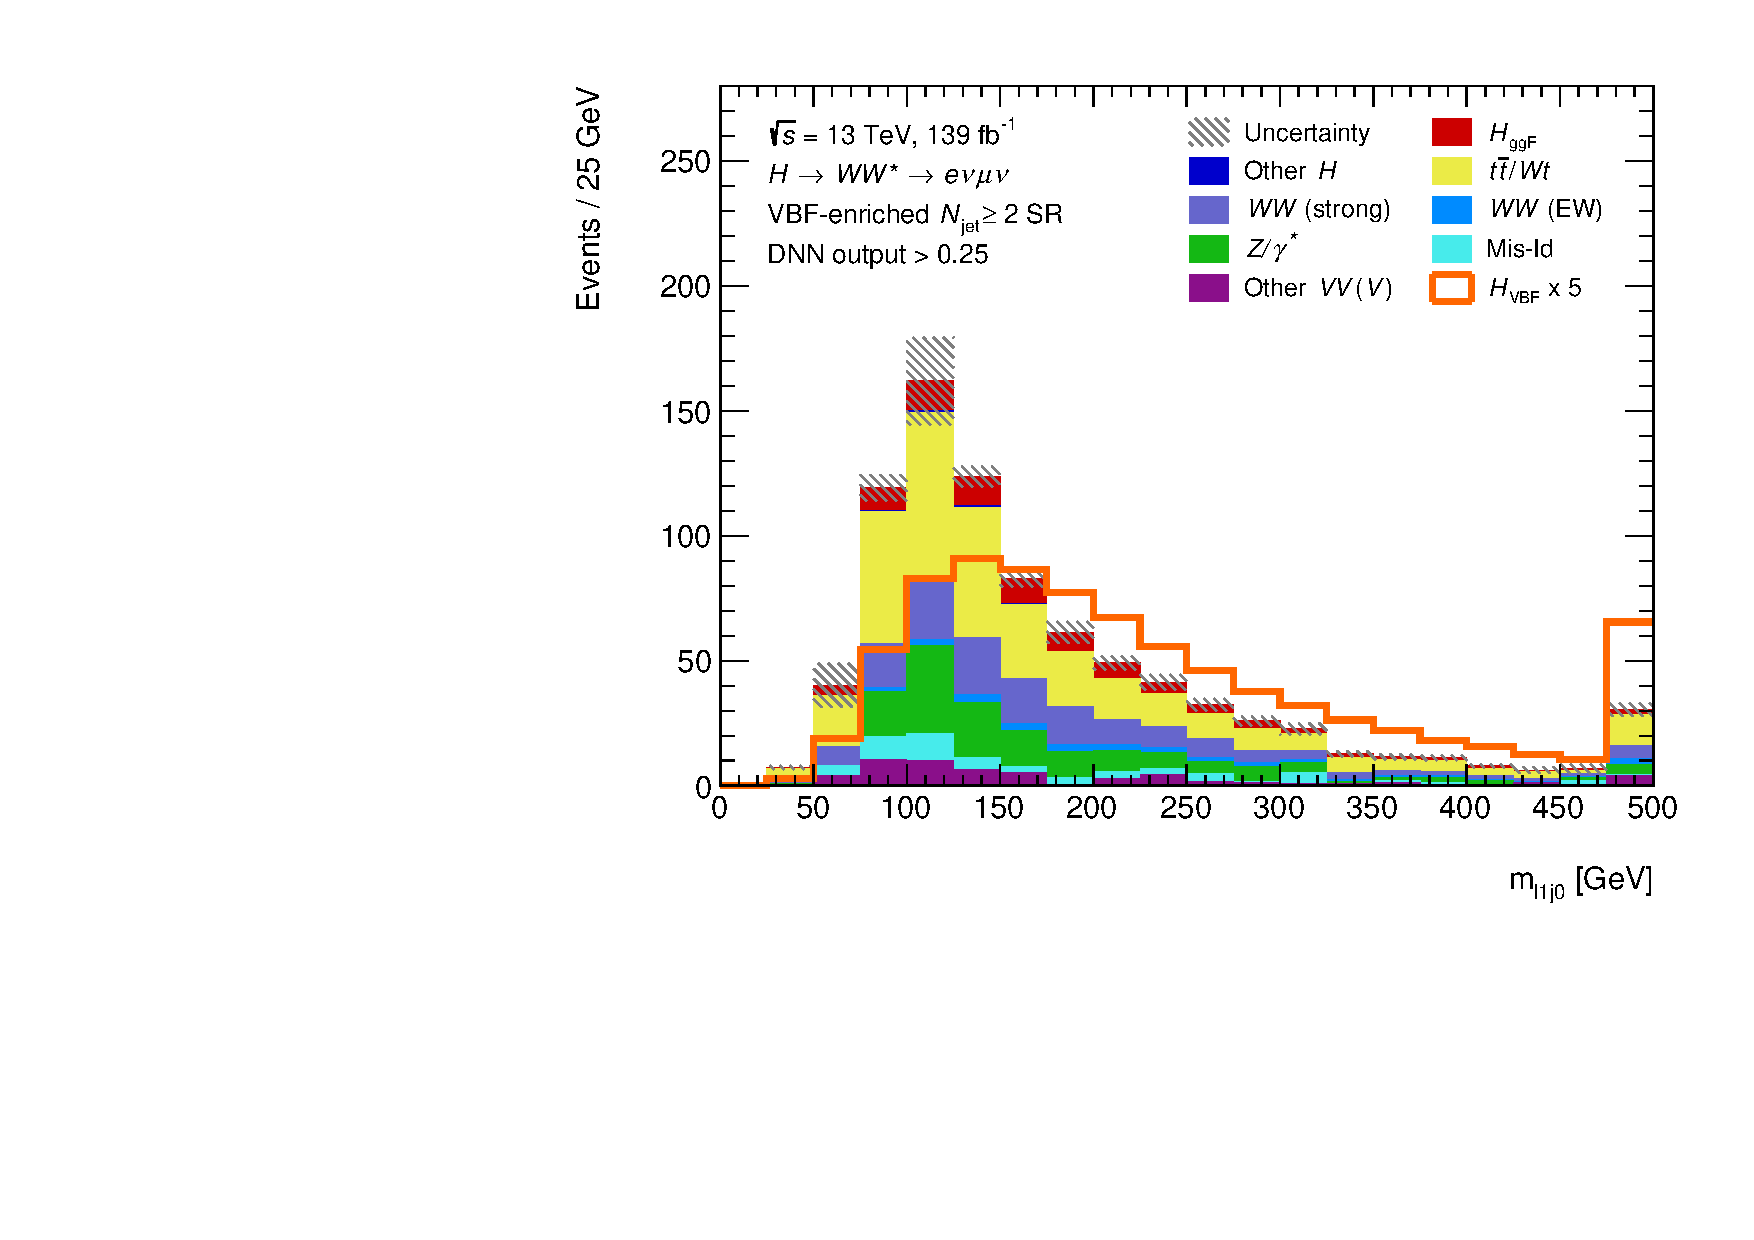
\includegraphics[width=0.32\textwidth]{figures/hww/dnn/blinded/run2-emme-CutVBFSR_DNN25-Ml1j0-lin.pdf} \hfill
            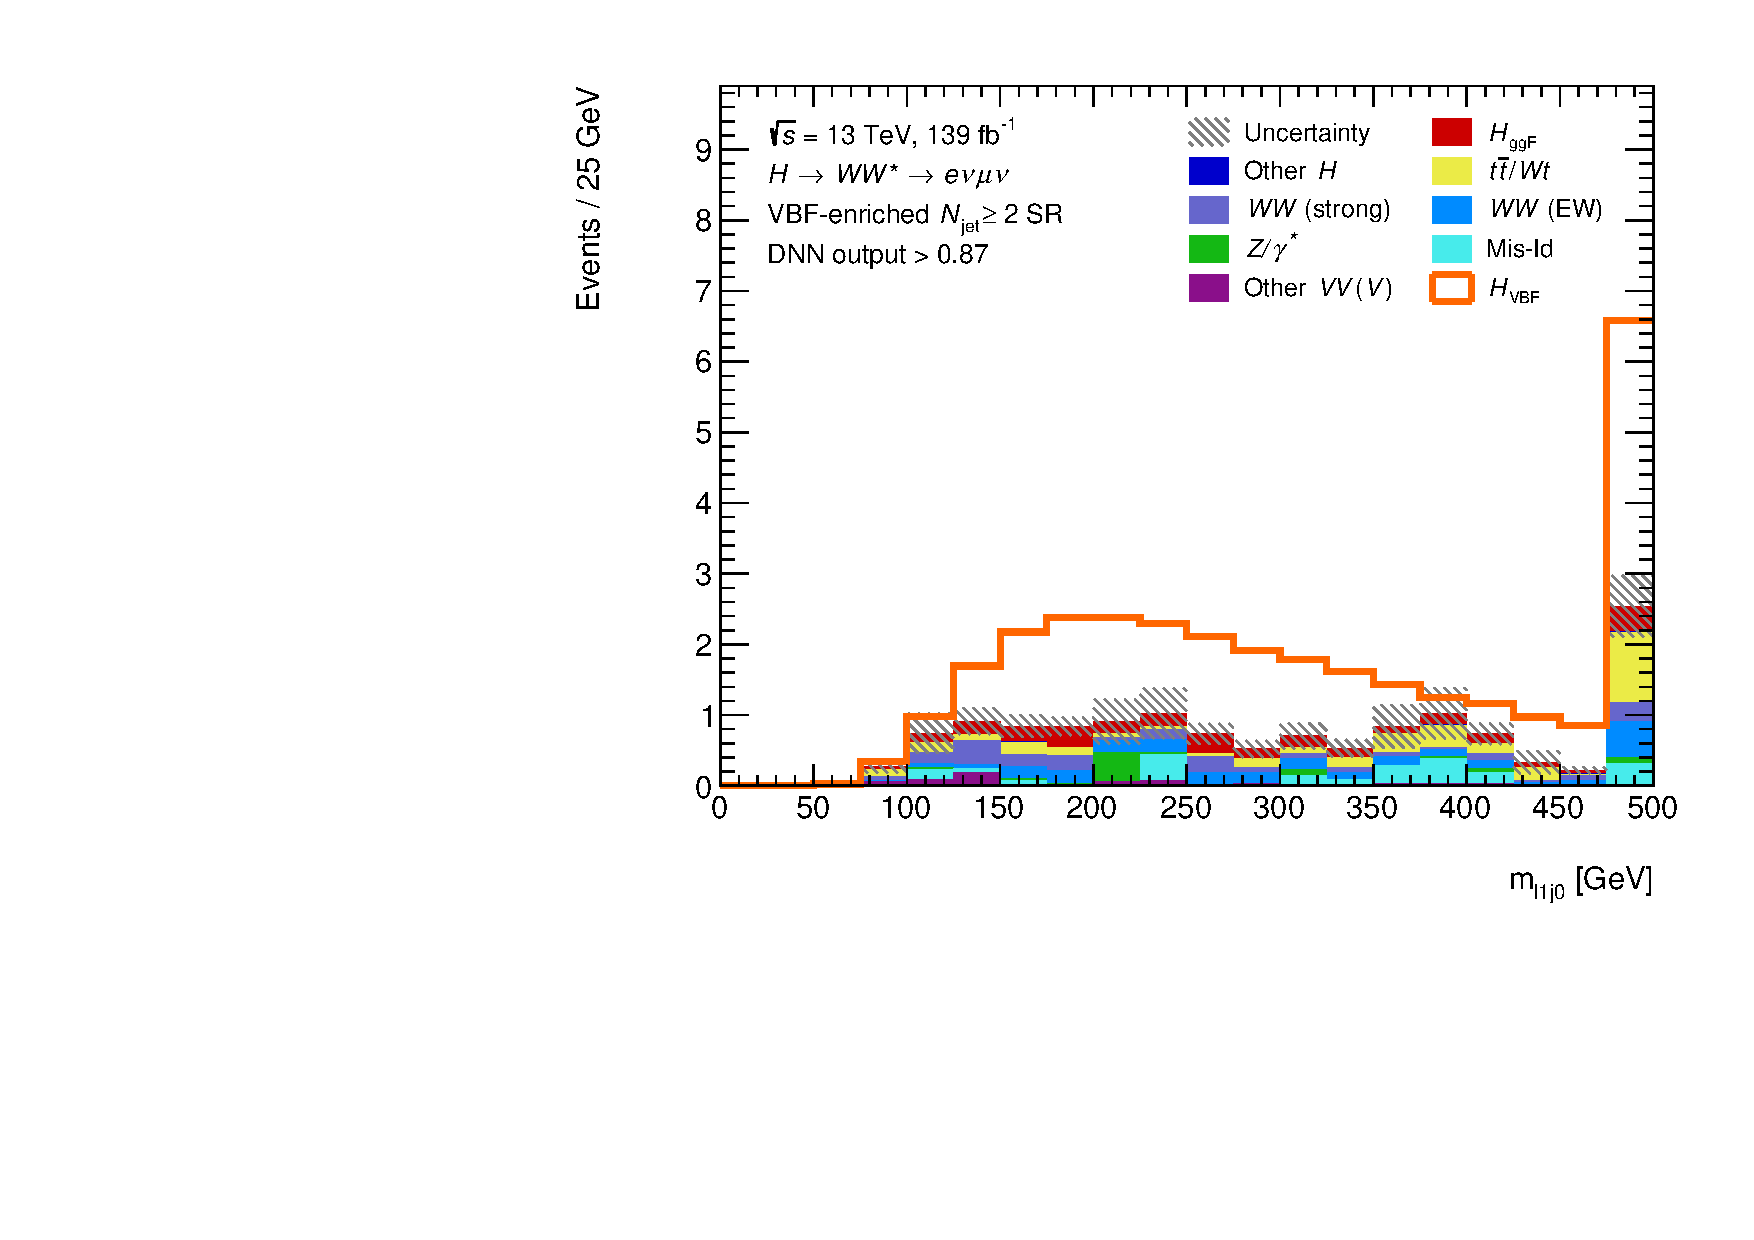
\includegraphics[width=0.32\textwidth]{figures/hww/dnn/blinded/run2-emme-CutVBFSR_DNN87-Ml1j0-lin.pdf}
        } \\
        \subfloat[$\mlonejtwo$]{
            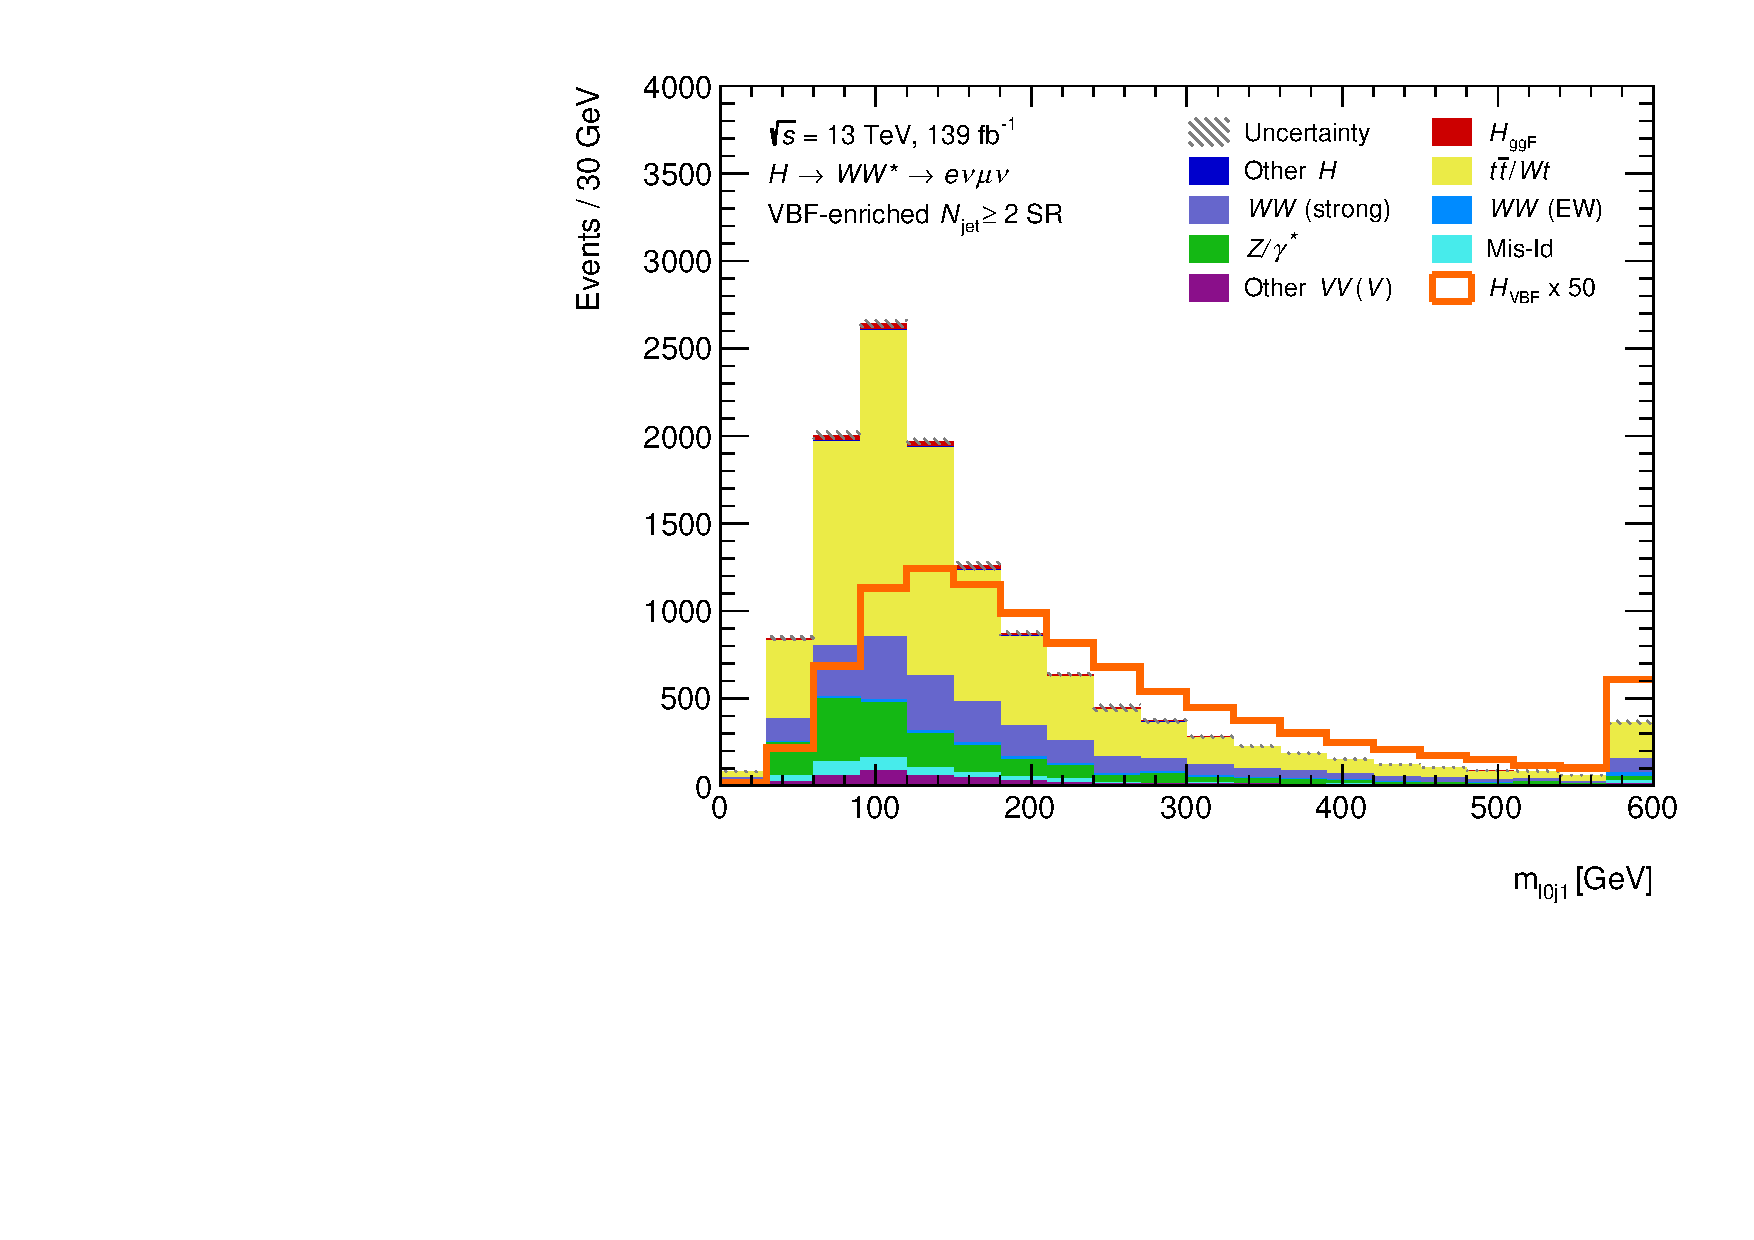
\includegraphics[width=0.32\textwidth]{figures/hww/dnn/blinded/run2-emme-CutVBF_SR-Ml0j1-lin.pdf} \hfill
            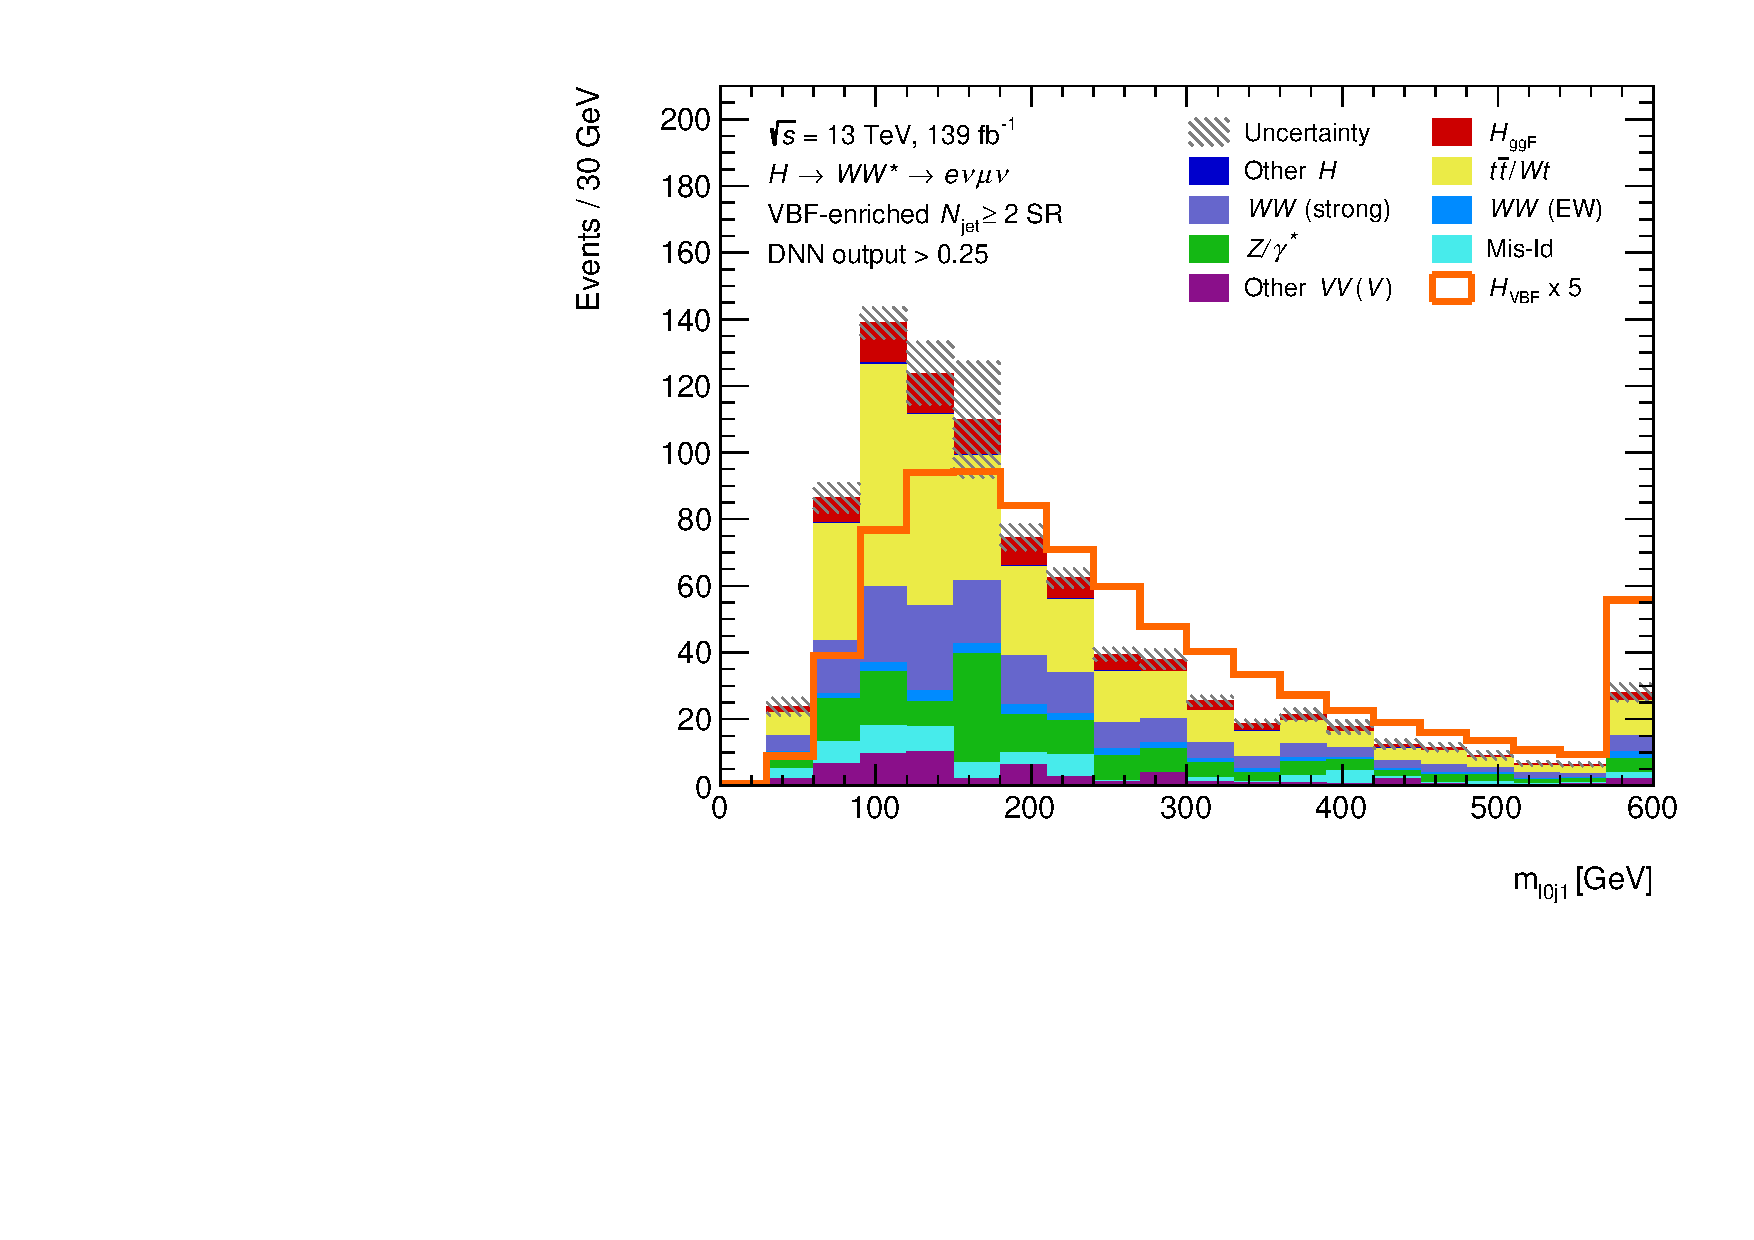
\includegraphics[width=0.32\textwidth]{figures/hww/dnn/blinded/run2-emme-CutVBFSR_DNN25-Ml0j1-lin.pdf} \hfill
            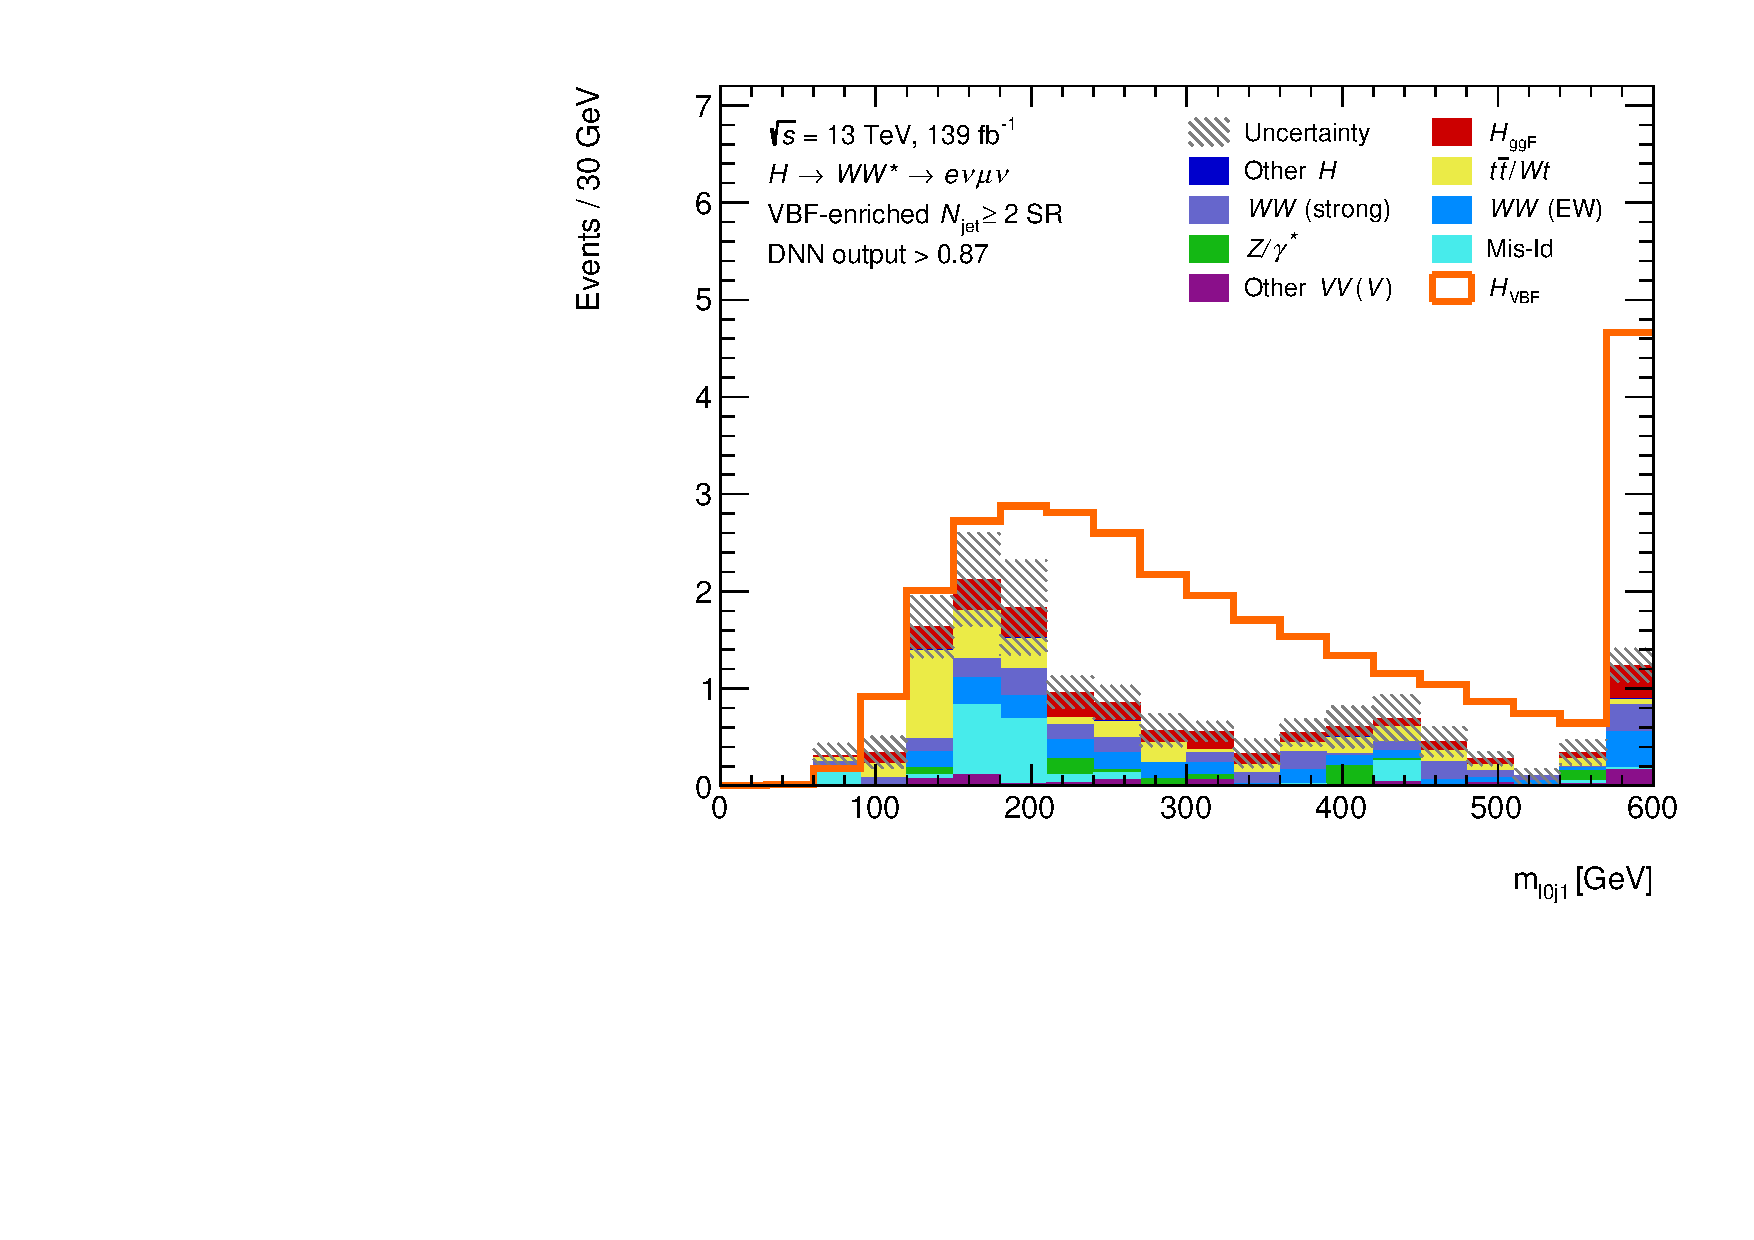
\includegraphics[width=0.32\textwidth]{figures/hww/dnn/blinded/run2-emme-CutVBFSR_DNN87-Ml0j1-lin.pdf}
        } \\
        \subfloat[$\mltwojtwo$]{
            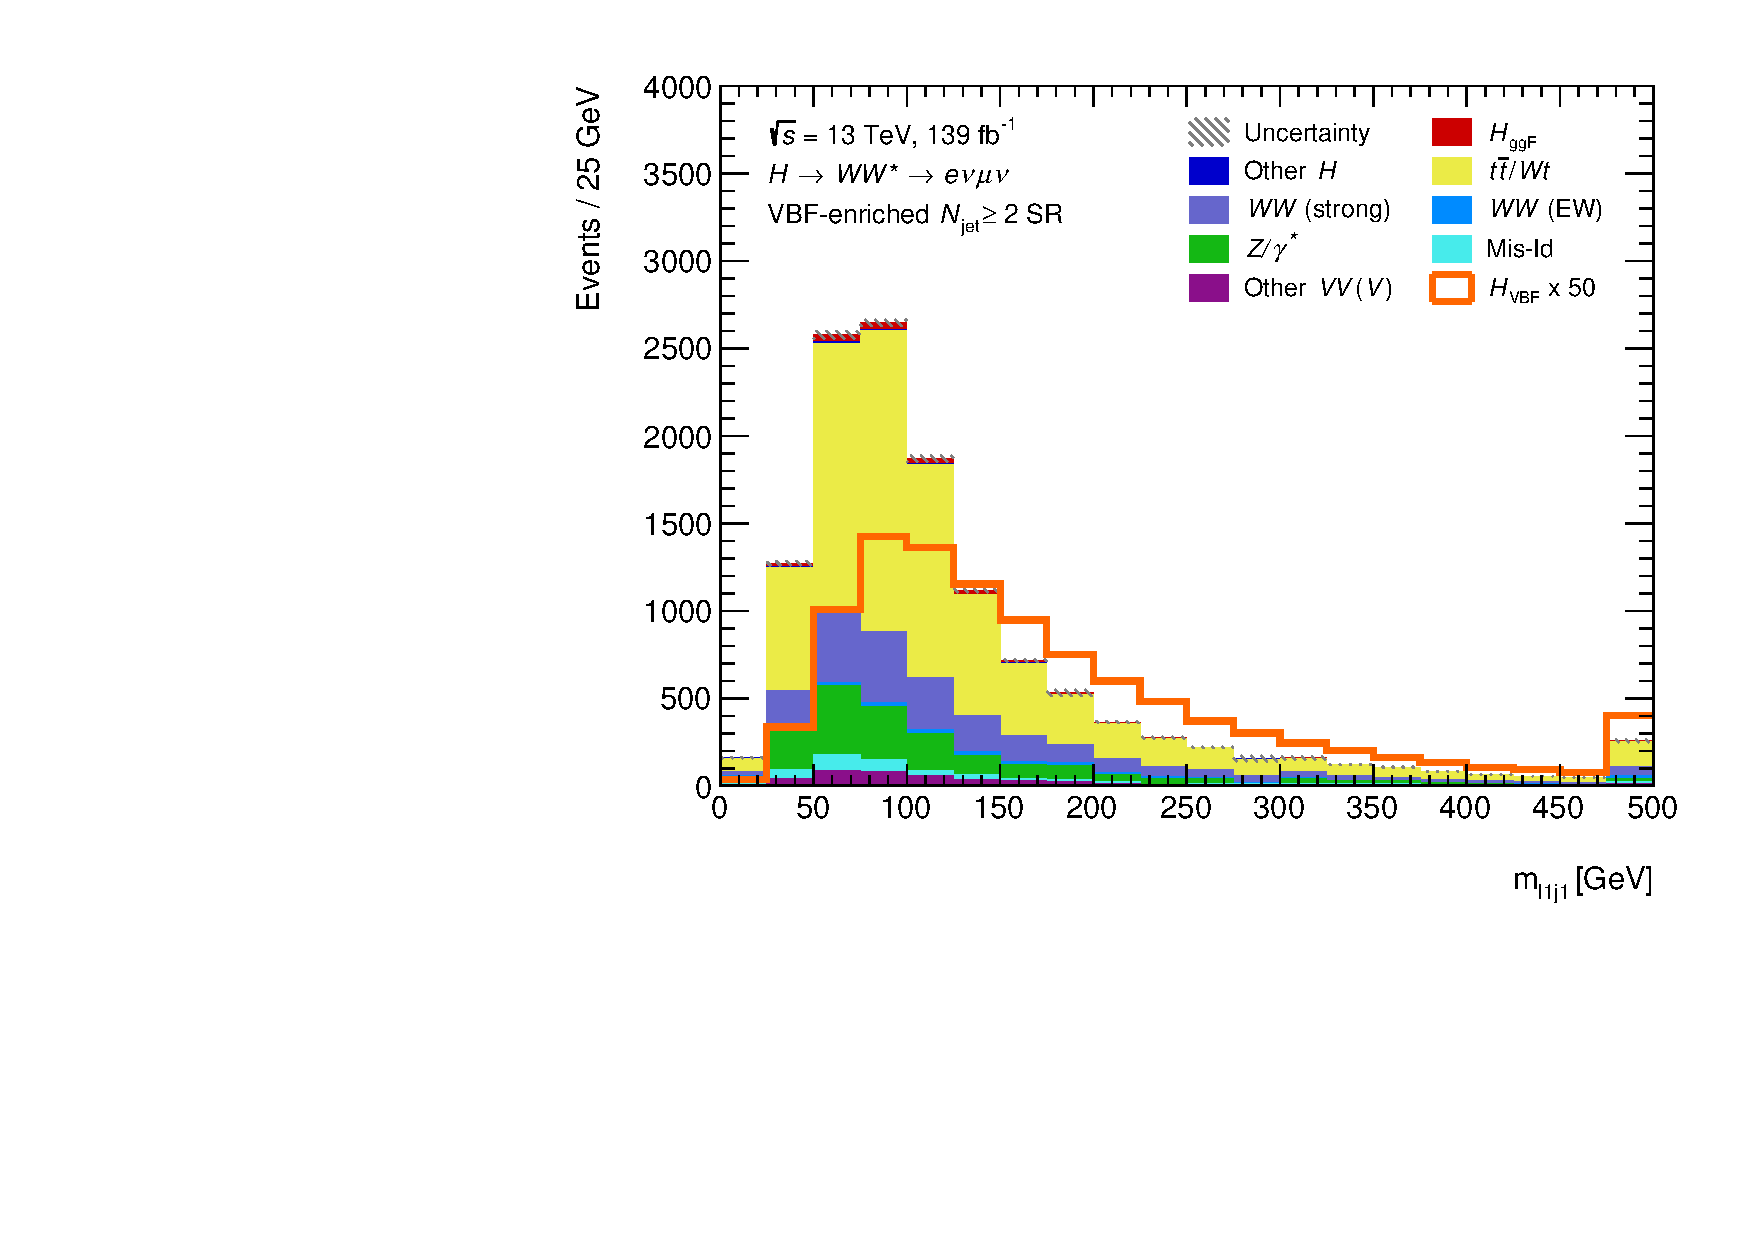
\includegraphics[width=0.32\textwidth]{figures/hww/dnn/blinded/run2-emme-CutVBF_SR-Ml1j1-lin.pdf} \hfill
            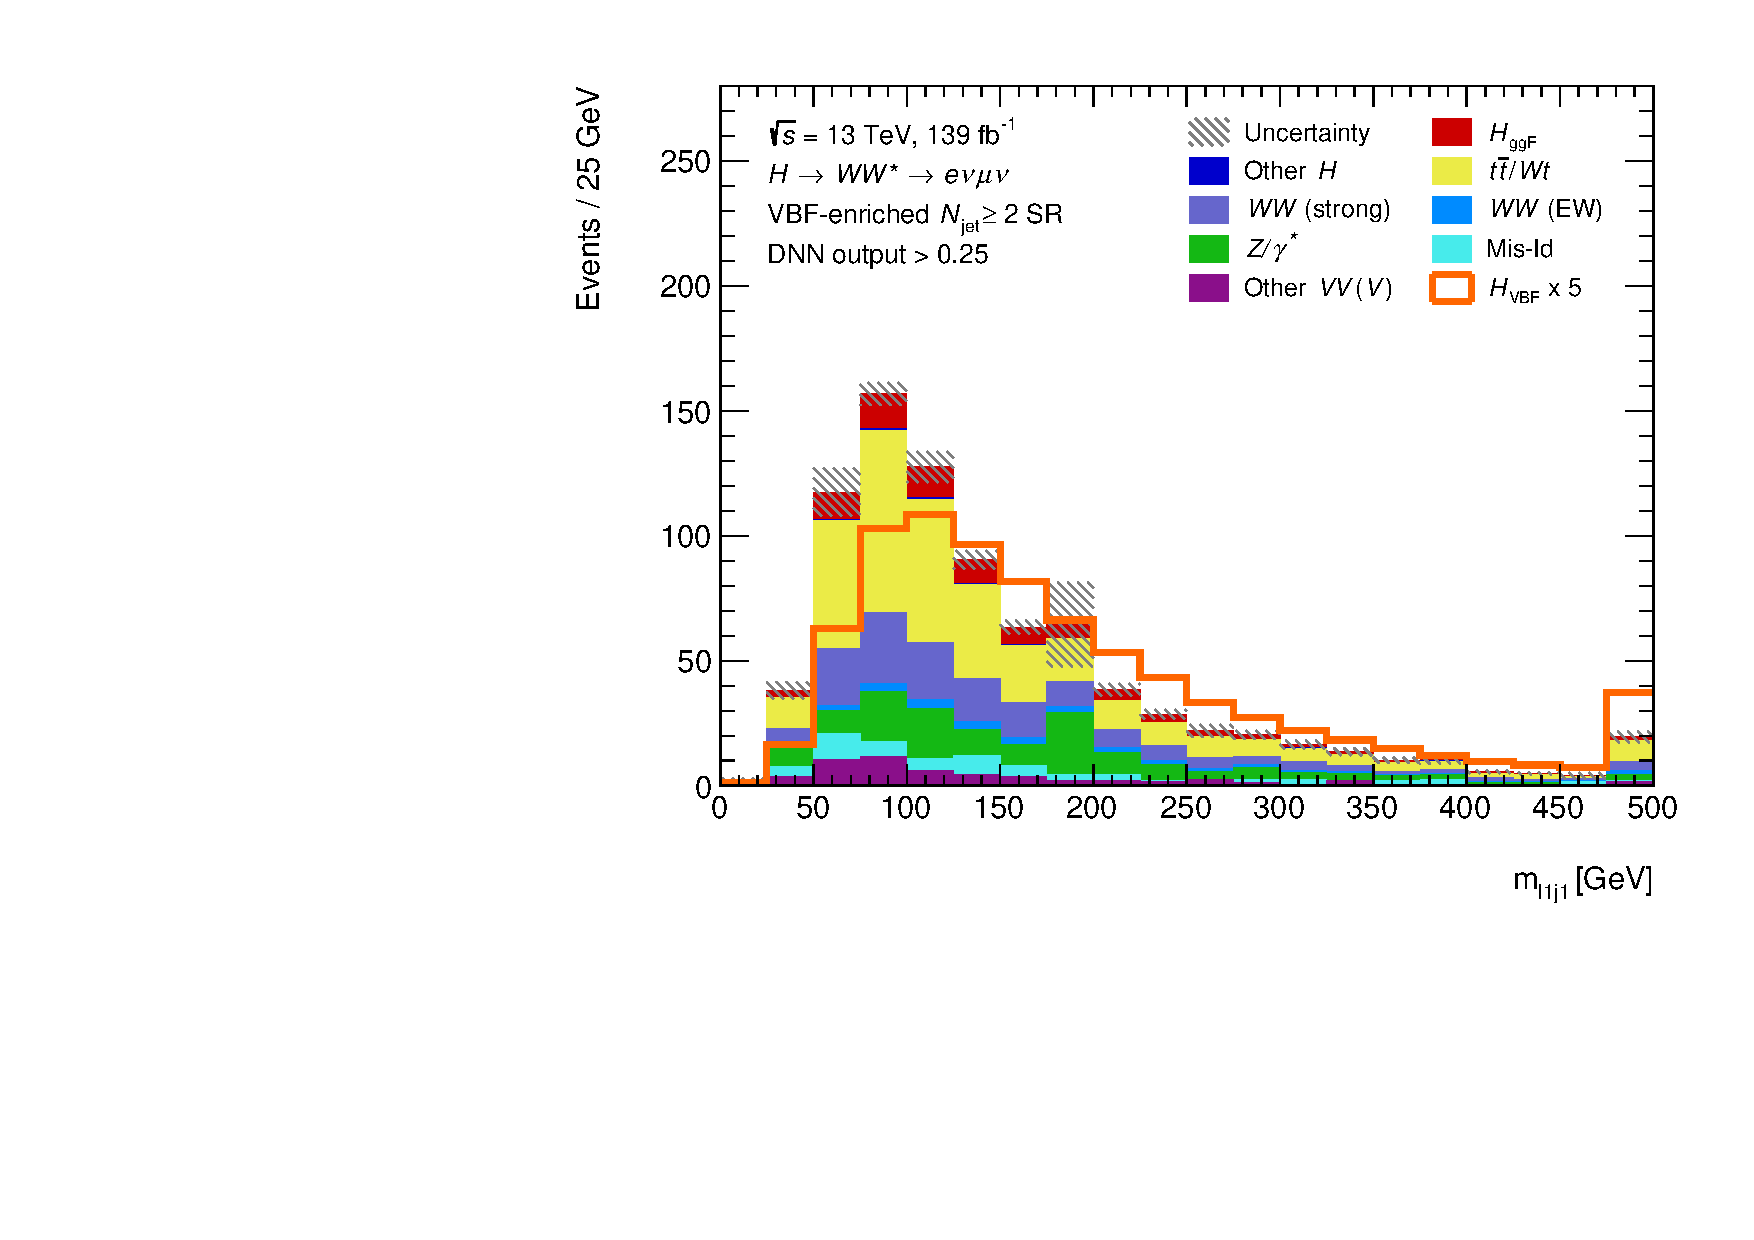
\includegraphics[width=0.32\textwidth]{figures/hww/dnn/blinded/run2-emme-CutVBFSR_DNN25-Ml1j1-lin.pdf} \hfill
            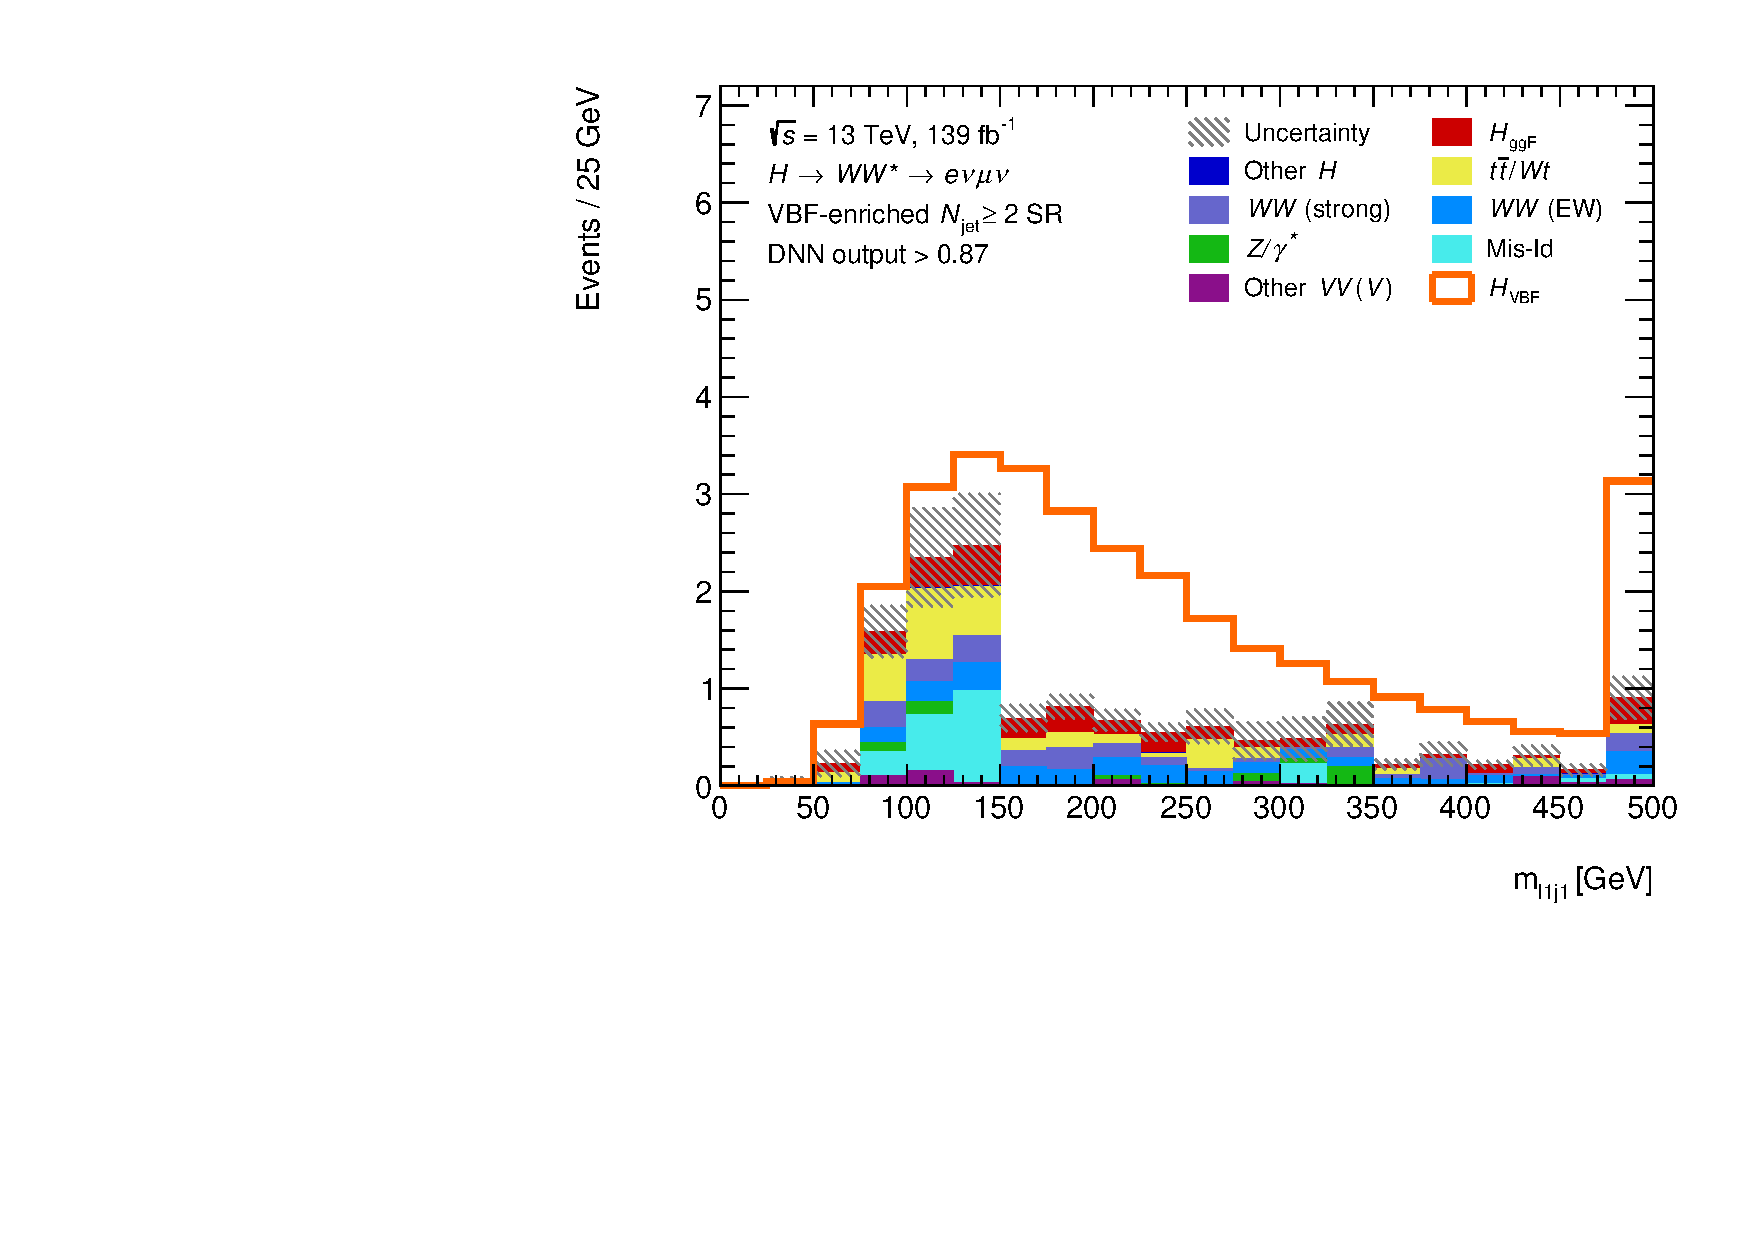
\includegraphics[width=0.32\textwidth]{figures/hww/dnn/blinded/run2-emme-CutVBFSR_DNN87-Ml1j1-lin.pdf}
        }
        {\caption[Distributions of $\mlonejone$, $\mltwojone$, $\mlonejtwo$, and $\mltwojtwo$ in the VBF \TwoJet signal region.]{Distributions of $\mlonejone$, $\mltwojone$, $\mlonejtwo$, and $\mltwojtwo$ in the VBF \TwoJet signal region.
                Each row corresponds to one variable with different selections made on the DNN output as indicated in the figure. The solid orange line shows the expected VBF signal scaled by a factor of (left) 50, (center) 5, and (right) without any scaling.
                \label{app:fig:dnn-inputs-vbf-top2} }}
    \end{figure}


    \begin{figure}[h]
        \centering
        \subfloat[$\pTjone$]{
            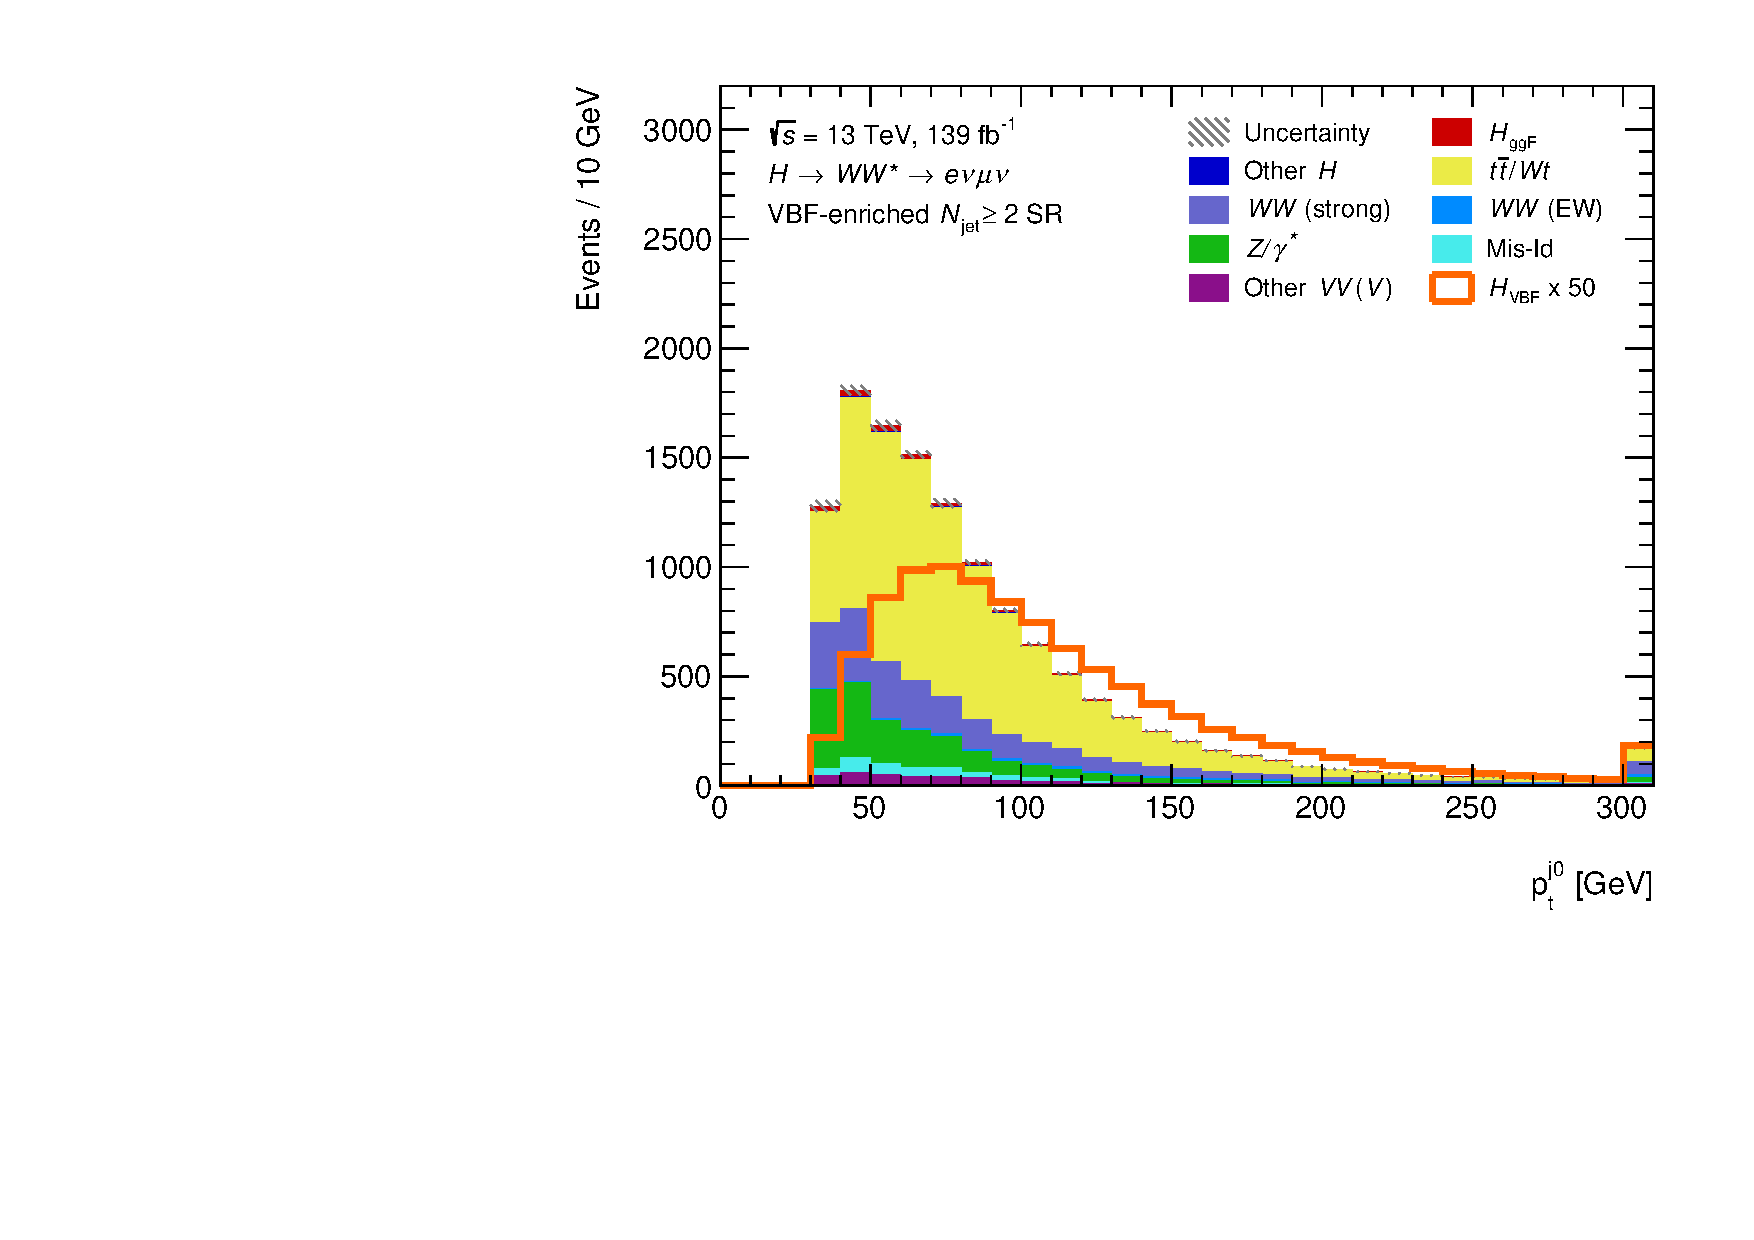
\includegraphics[width=0.32\textwidth]{figures/hww/dnn/blinded/run2-emme-CutVBF_SR-leadJetPt-lin.pdf} \hfill
            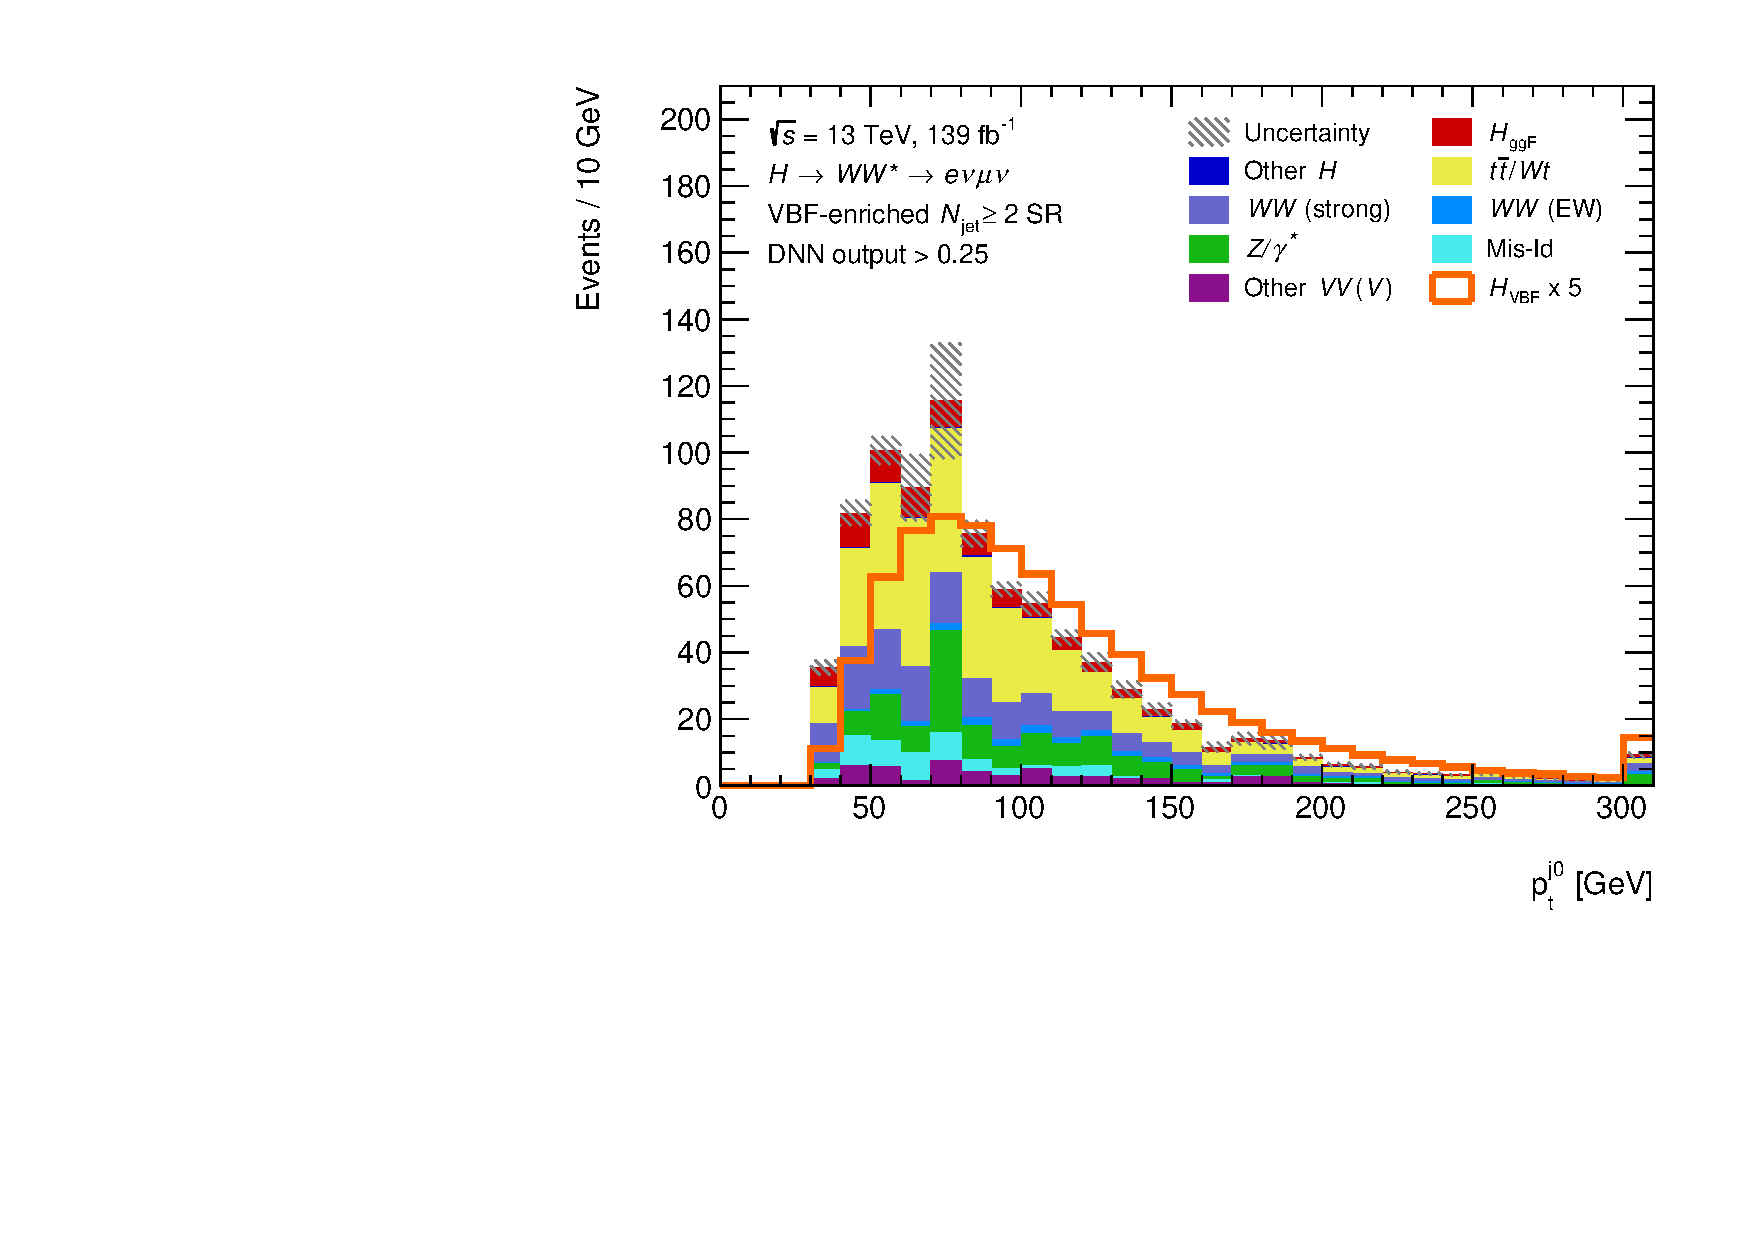
\includegraphics[width=0.32\textwidth]{figures/hww/dnn/blinded/run2-emme-CutVBFSR_DNN25-leadJetPt-lin.pdf} \hfill
            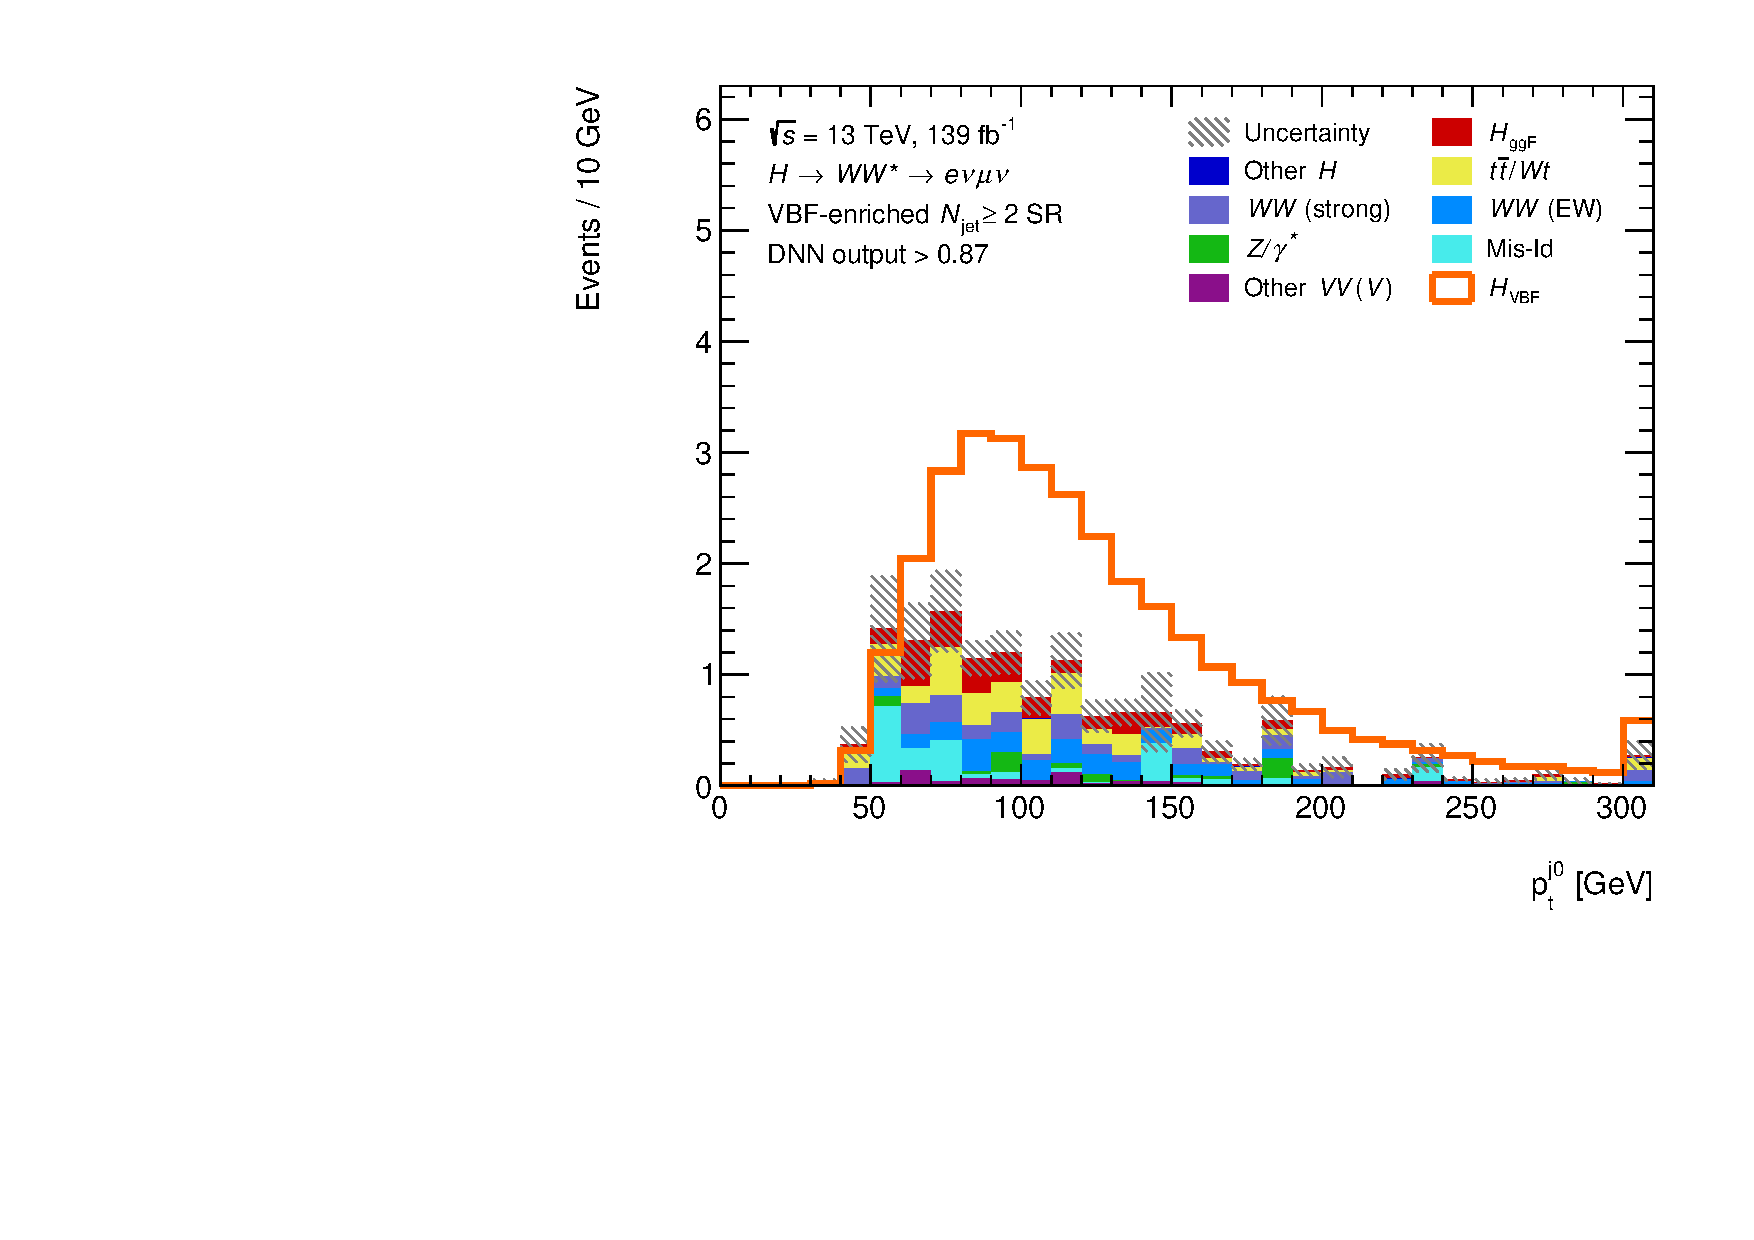
\includegraphics[width=0.32\textwidth]{figures/hww/dnn/blinded/run2-emme-CutVBFSR_DNN87-leadJetPt-lin.pdf}
        } \\
        \subfloat[$\pTjtwo$]{
            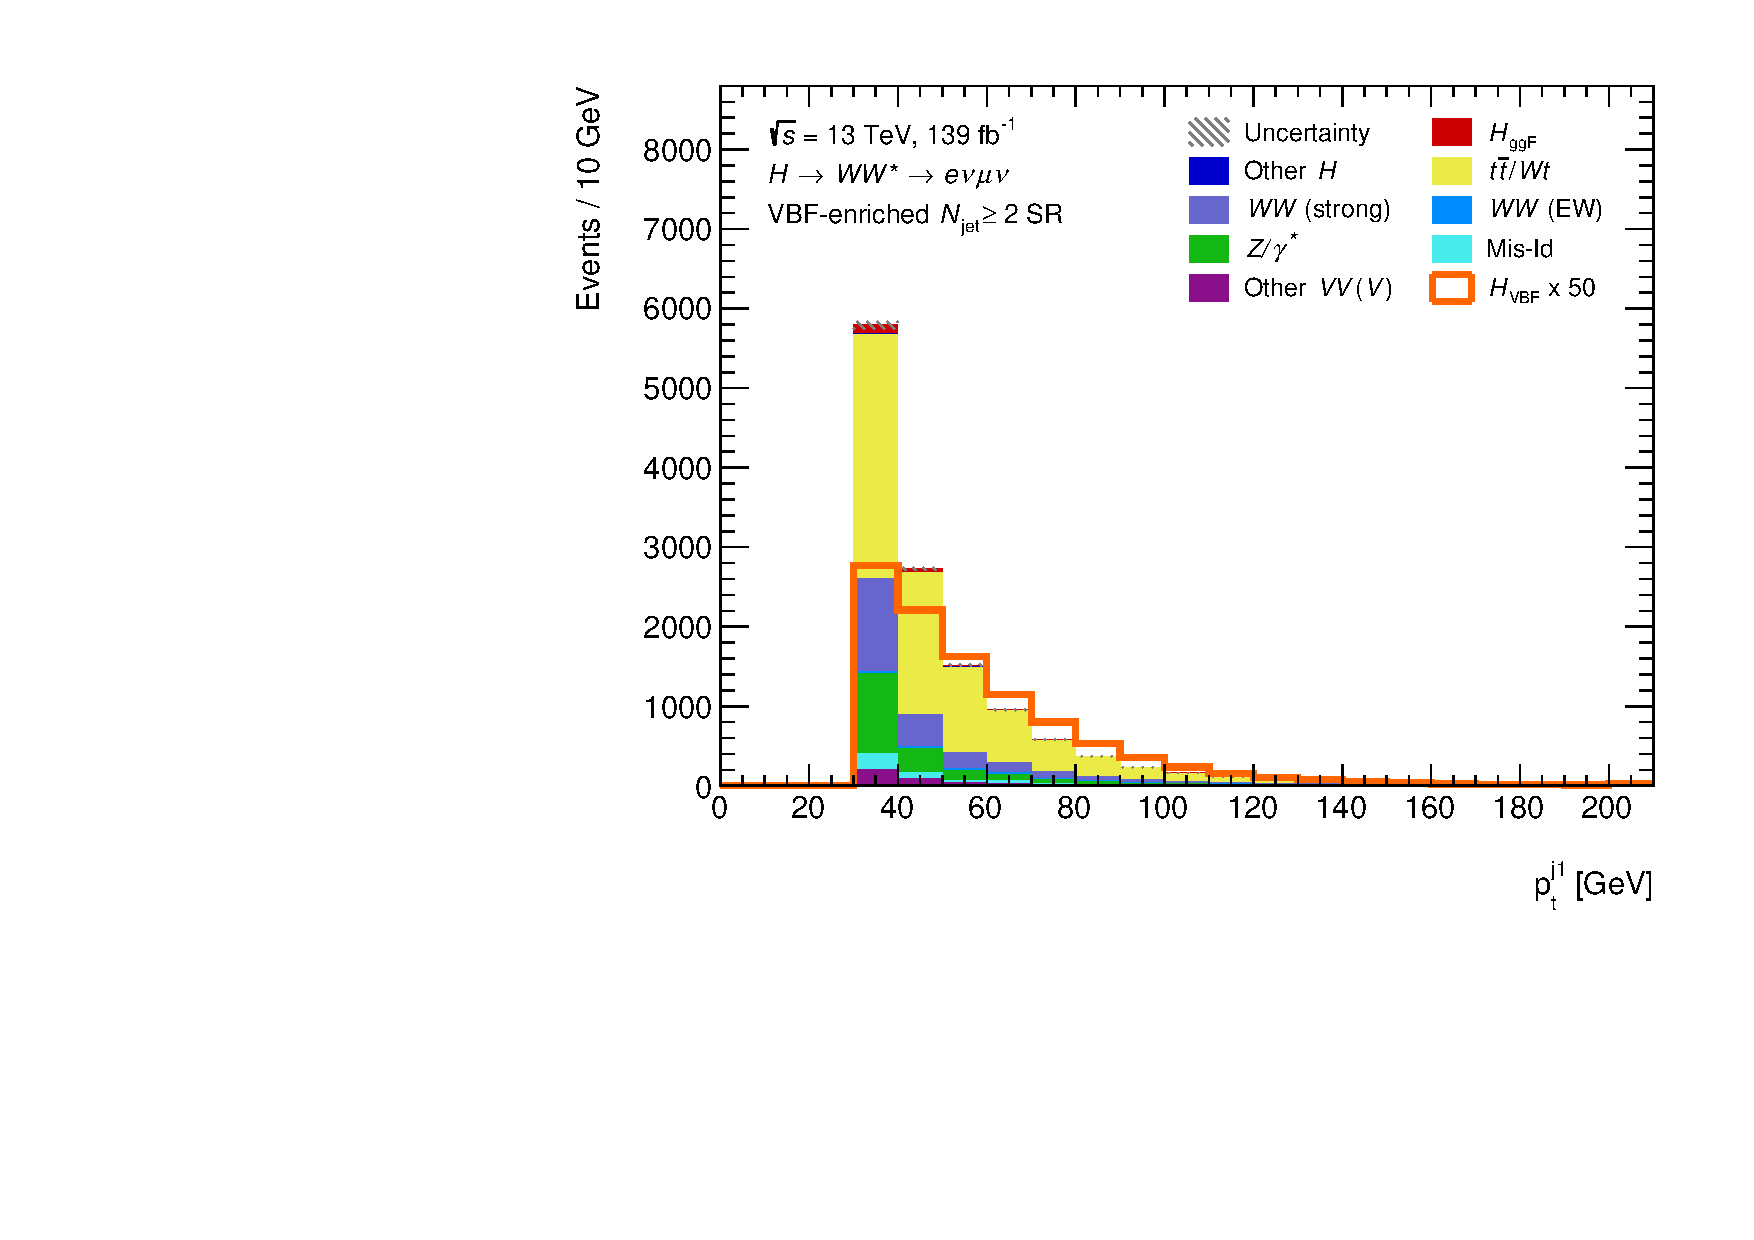
\includegraphics[width=0.32\textwidth]{figures/hww/dnn/blinded/run2-emme-CutVBF_SR-subleadJetPt-lin.pdf} \hfill
            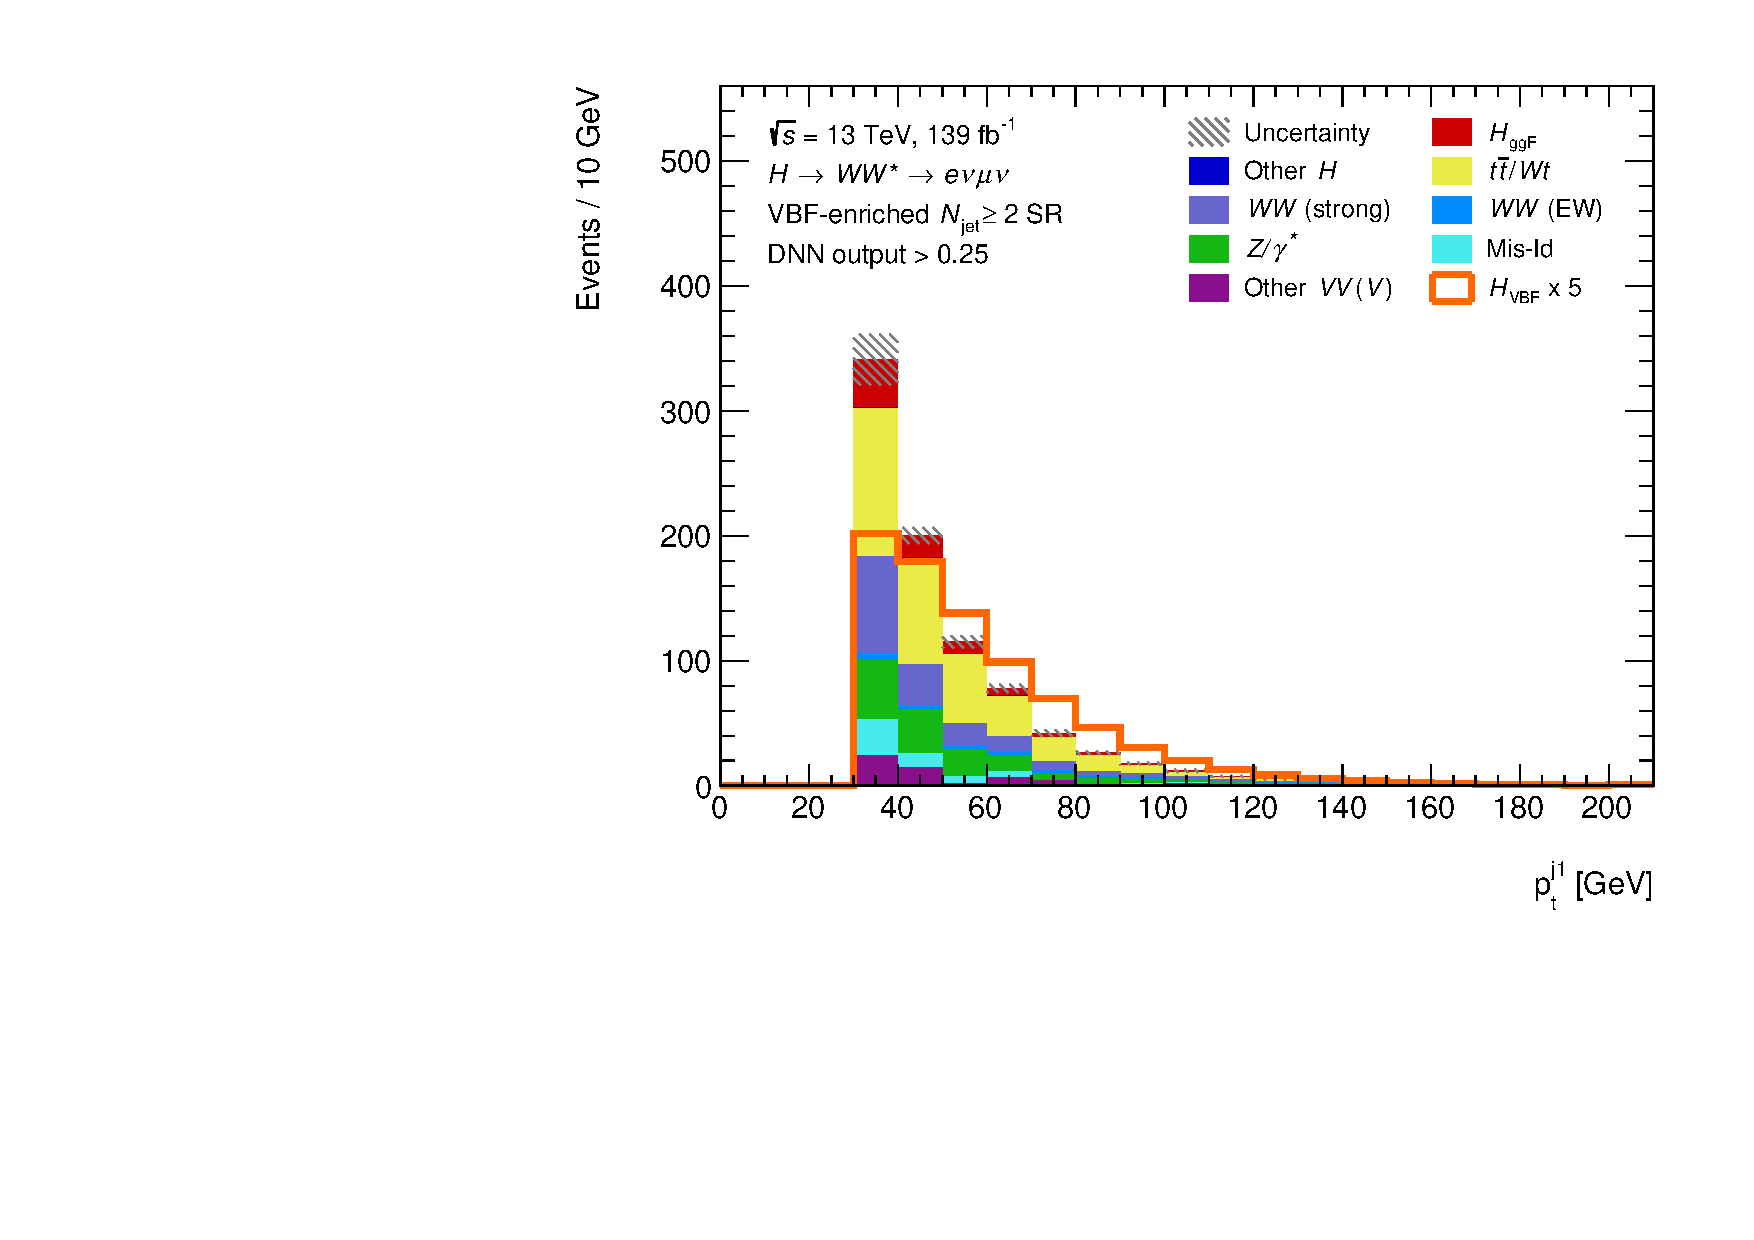
\includegraphics[width=0.32\textwidth]{figures/hww/dnn/blinded/run2-emme-CutVBFSR_DNN25-subleadJetPt-lin.pdf} \hfill
            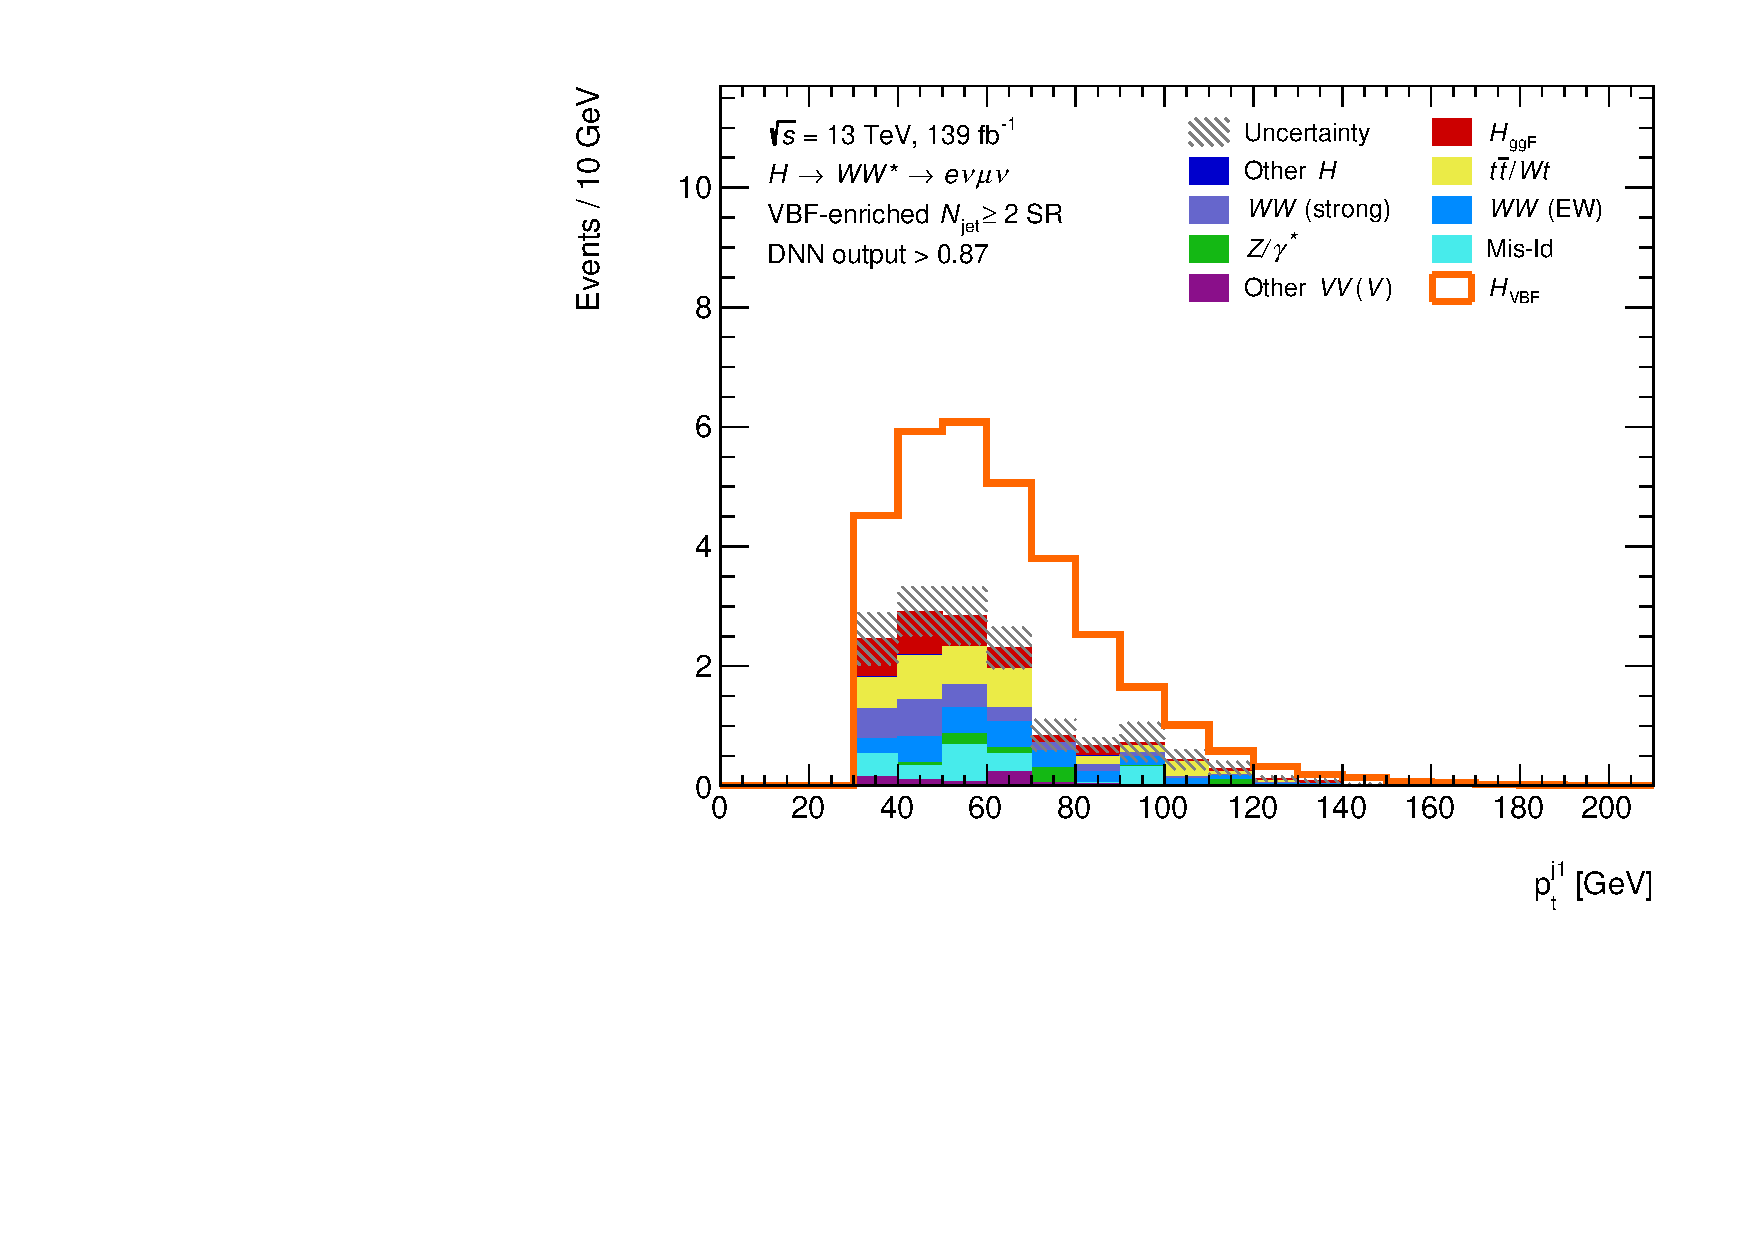
\includegraphics[width=0.32\textwidth]{figures/hww/dnn/blinded/run2-emme-CutVBFSR_DNN87-subleadJetPt-lin.pdf}
        } \\
        \subfloat[$\pTjthree$]{
            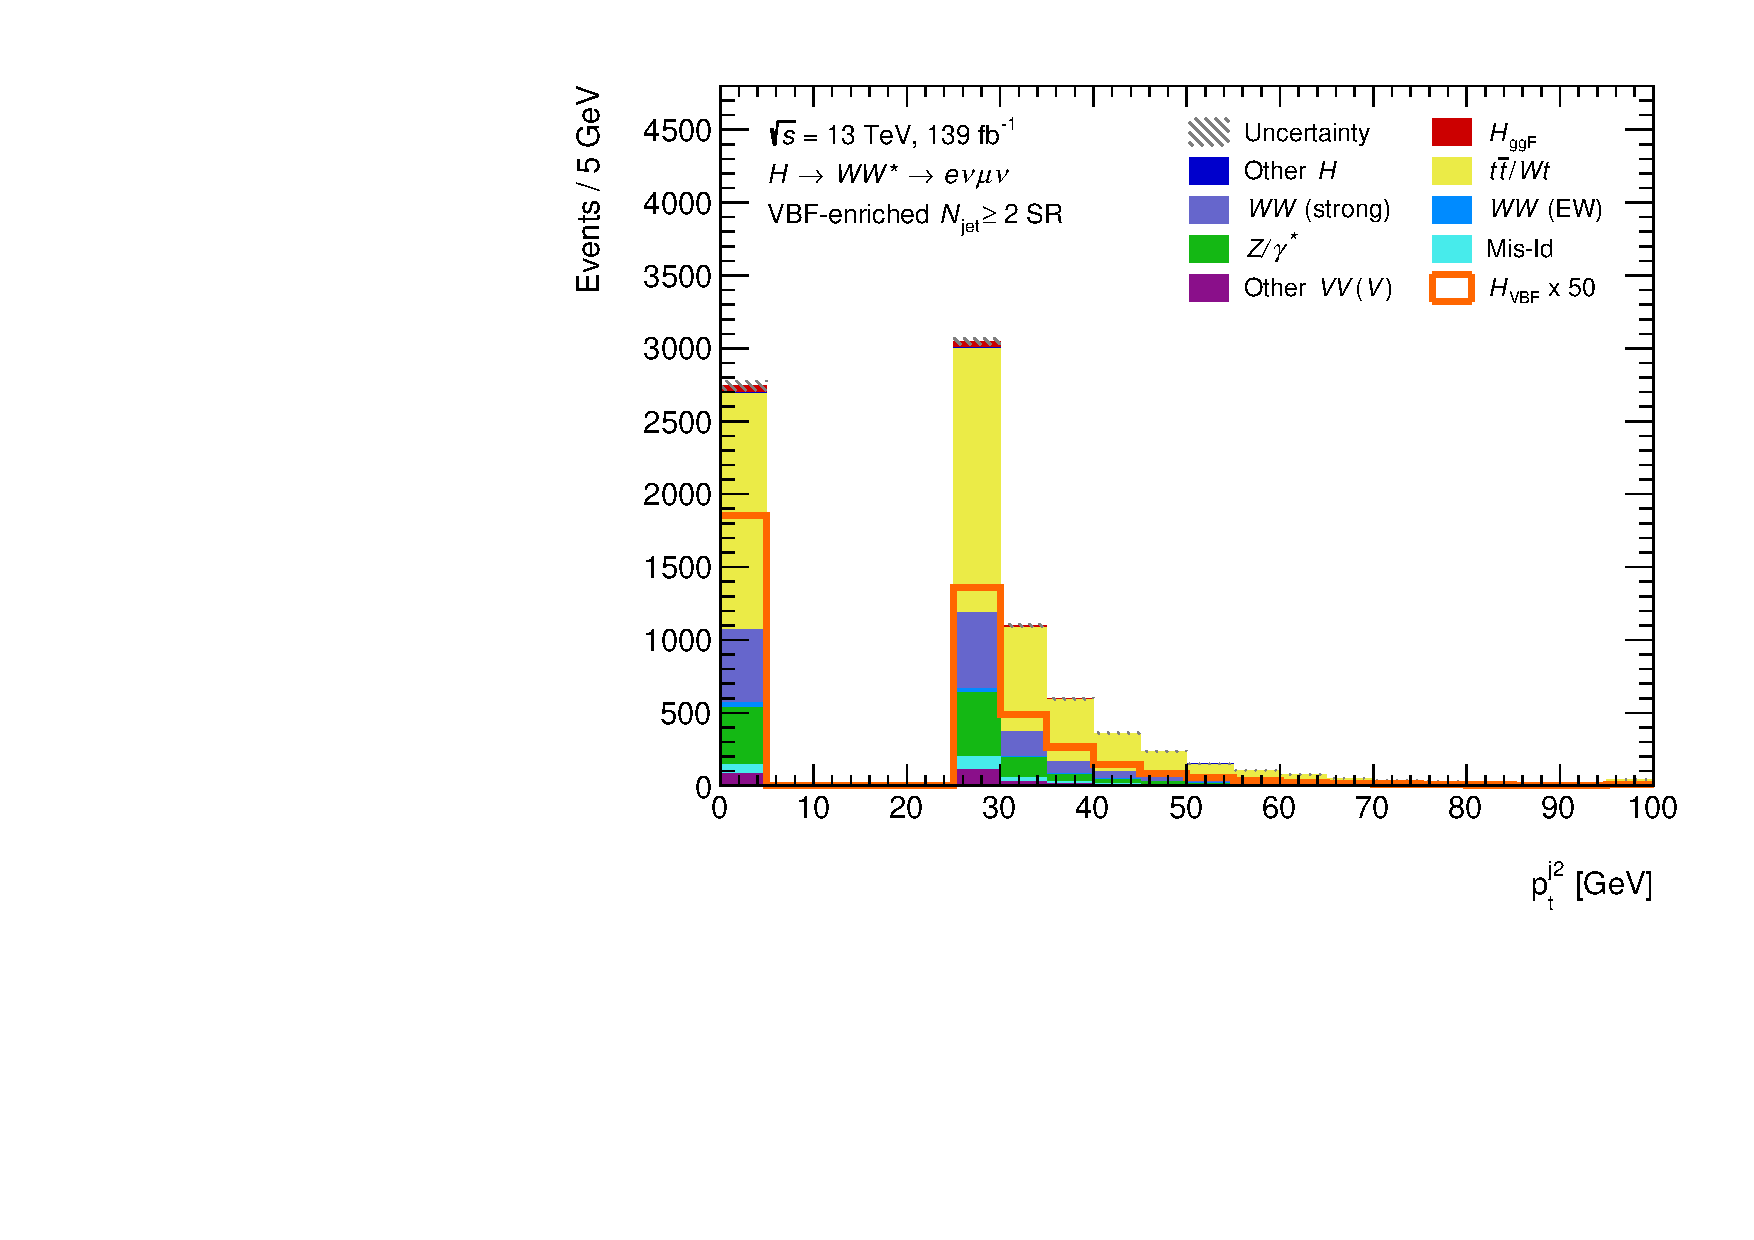
\includegraphics[width=0.32\textwidth]{figures/hww/dnn/blinded/run2-emme-CutVBF_SR-thirdJetPt-lin.pdf} \hfill
            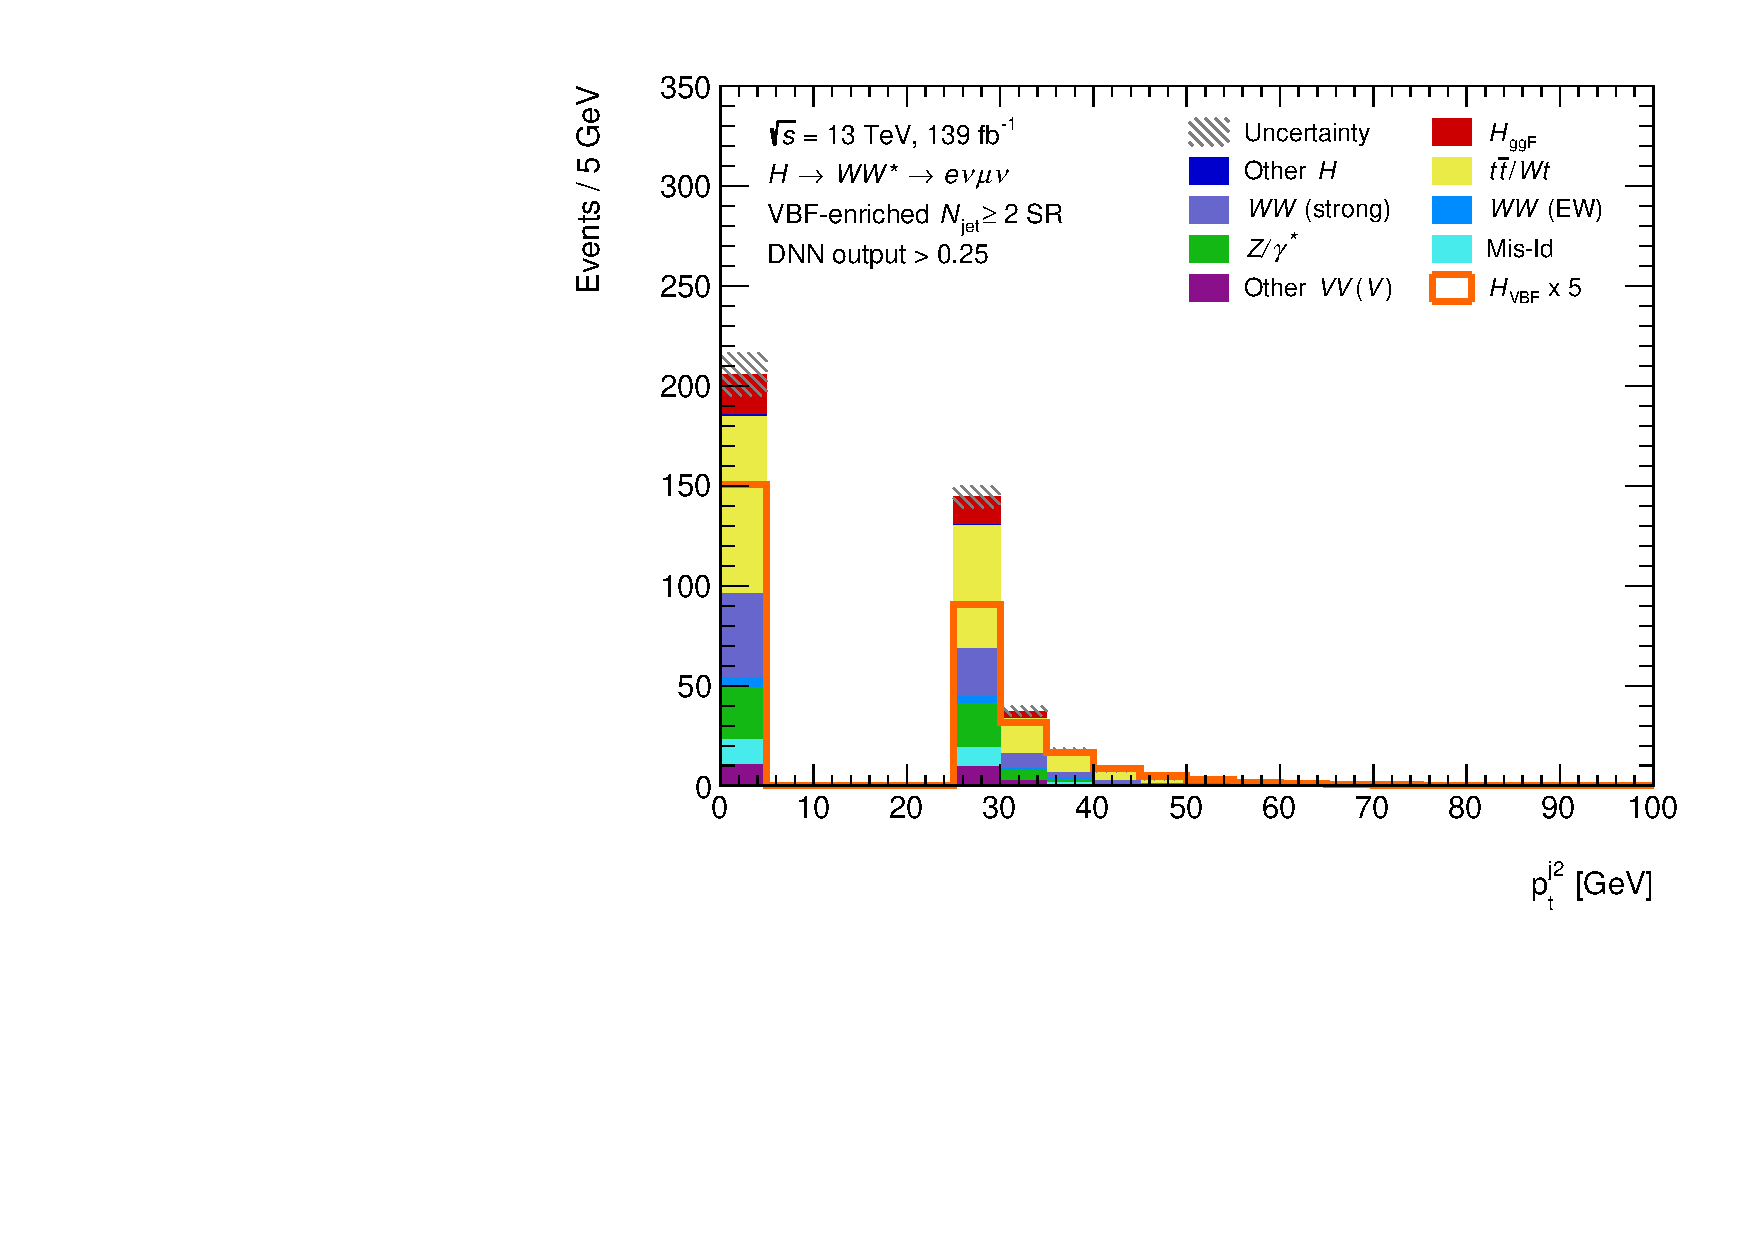
\includegraphics[width=0.32\textwidth]{figures/hww/dnn/blinded/run2-emme-CutVBFSR_DNN25-thirdJetPt-lin.pdf} \hfill
            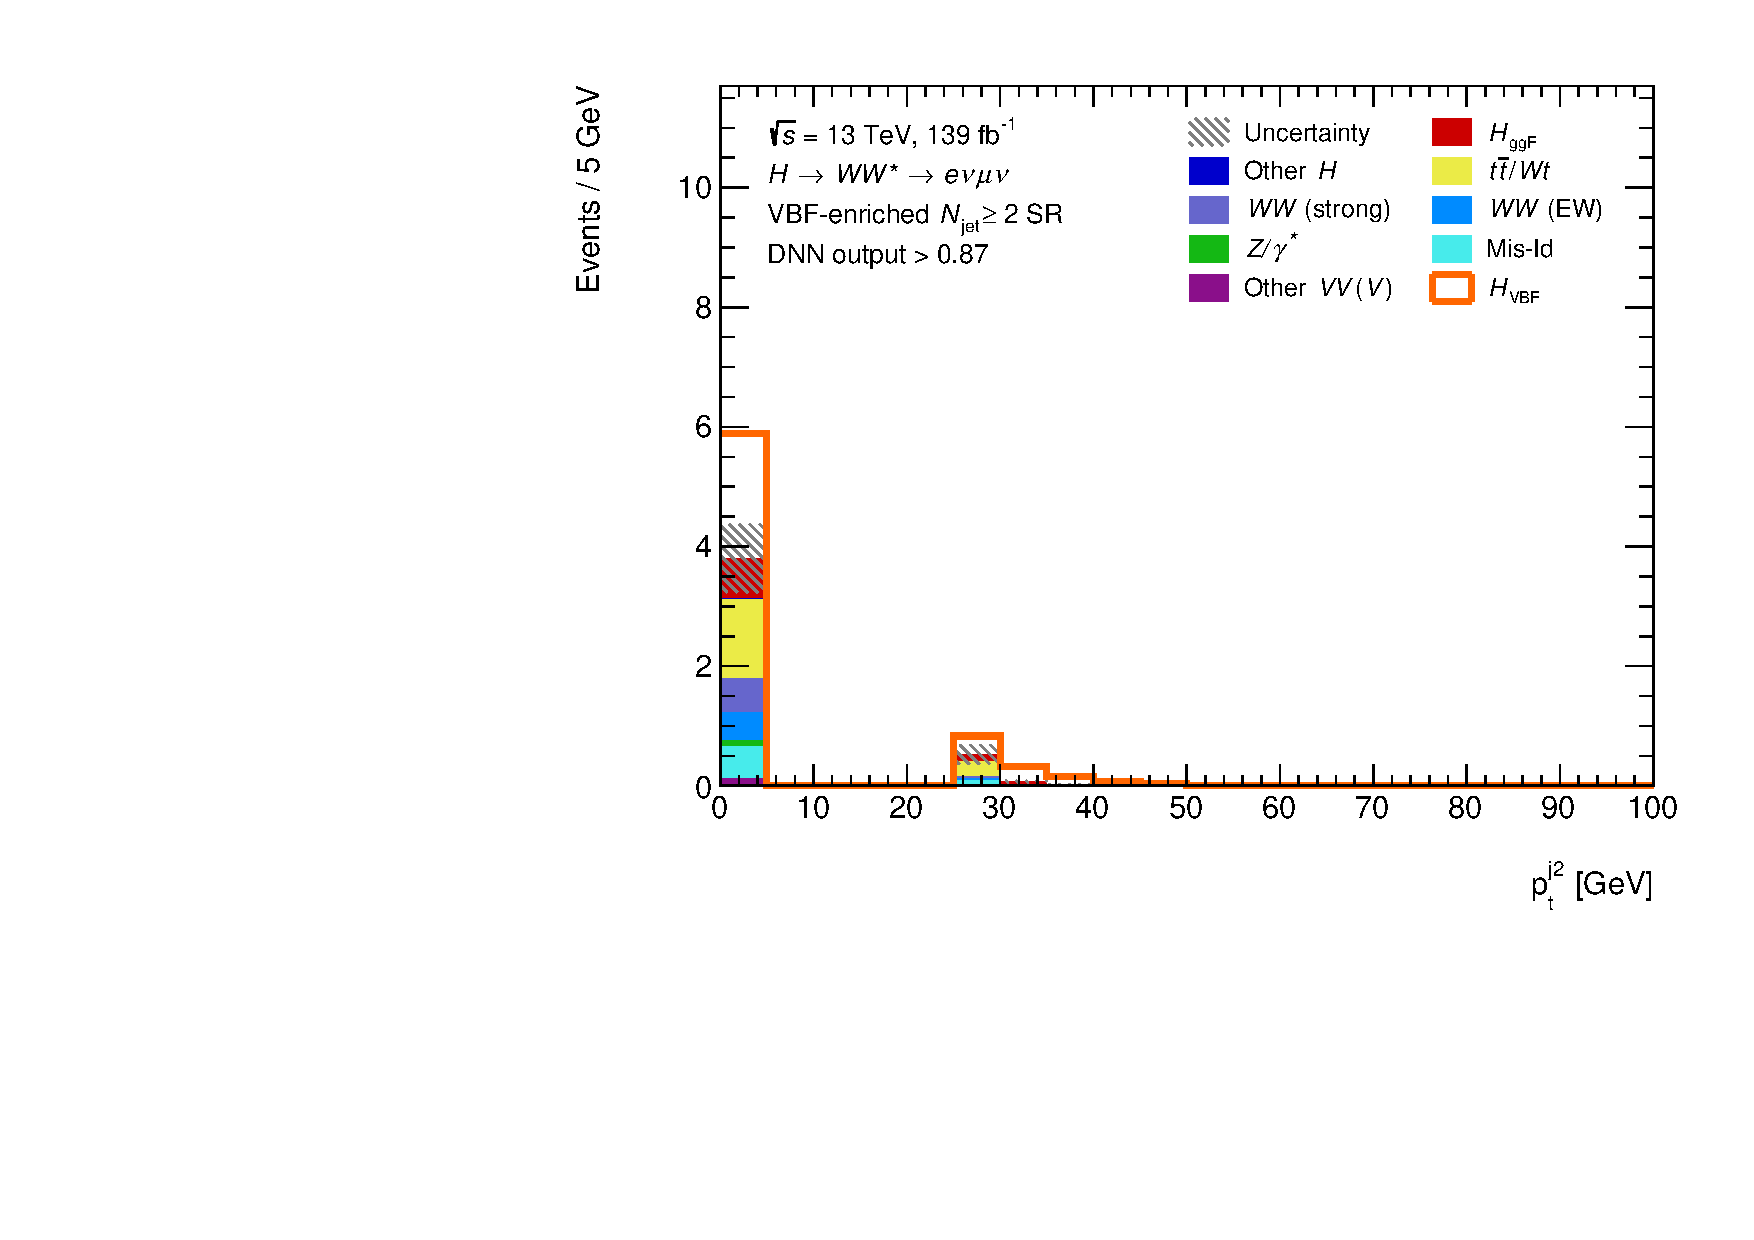
\includegraphics[width=0.32\textwidth]{figures/hww/dnn/blinded/run2-emme-CutVBFSR_DNN87-thirdJetPt-lin.pdf}
        }
        {\caption[Distributions of $\pTjone$, $\pTjtwo$, and $\pTjthree$ in the VBF \TwoJet signal region.]{Distributions of $\pTjone$, $\pTjtwo$, and $\pTjthree$ in the VBF \TwoJet signal region.
                Each row corresponds to one variable with different selections made on the DNN output as indicated in the figure. The solid orange line shows the expected VBF signal scaled by a factor of (left) 50, (center) 5, and (right) without any scaling.
                \label{app:fig:dnn-inputs-vbf-top3}}}
    \end{figure}


    \begin{figure}[h]
        \centering
        \subfloat[$\dphill$]{
            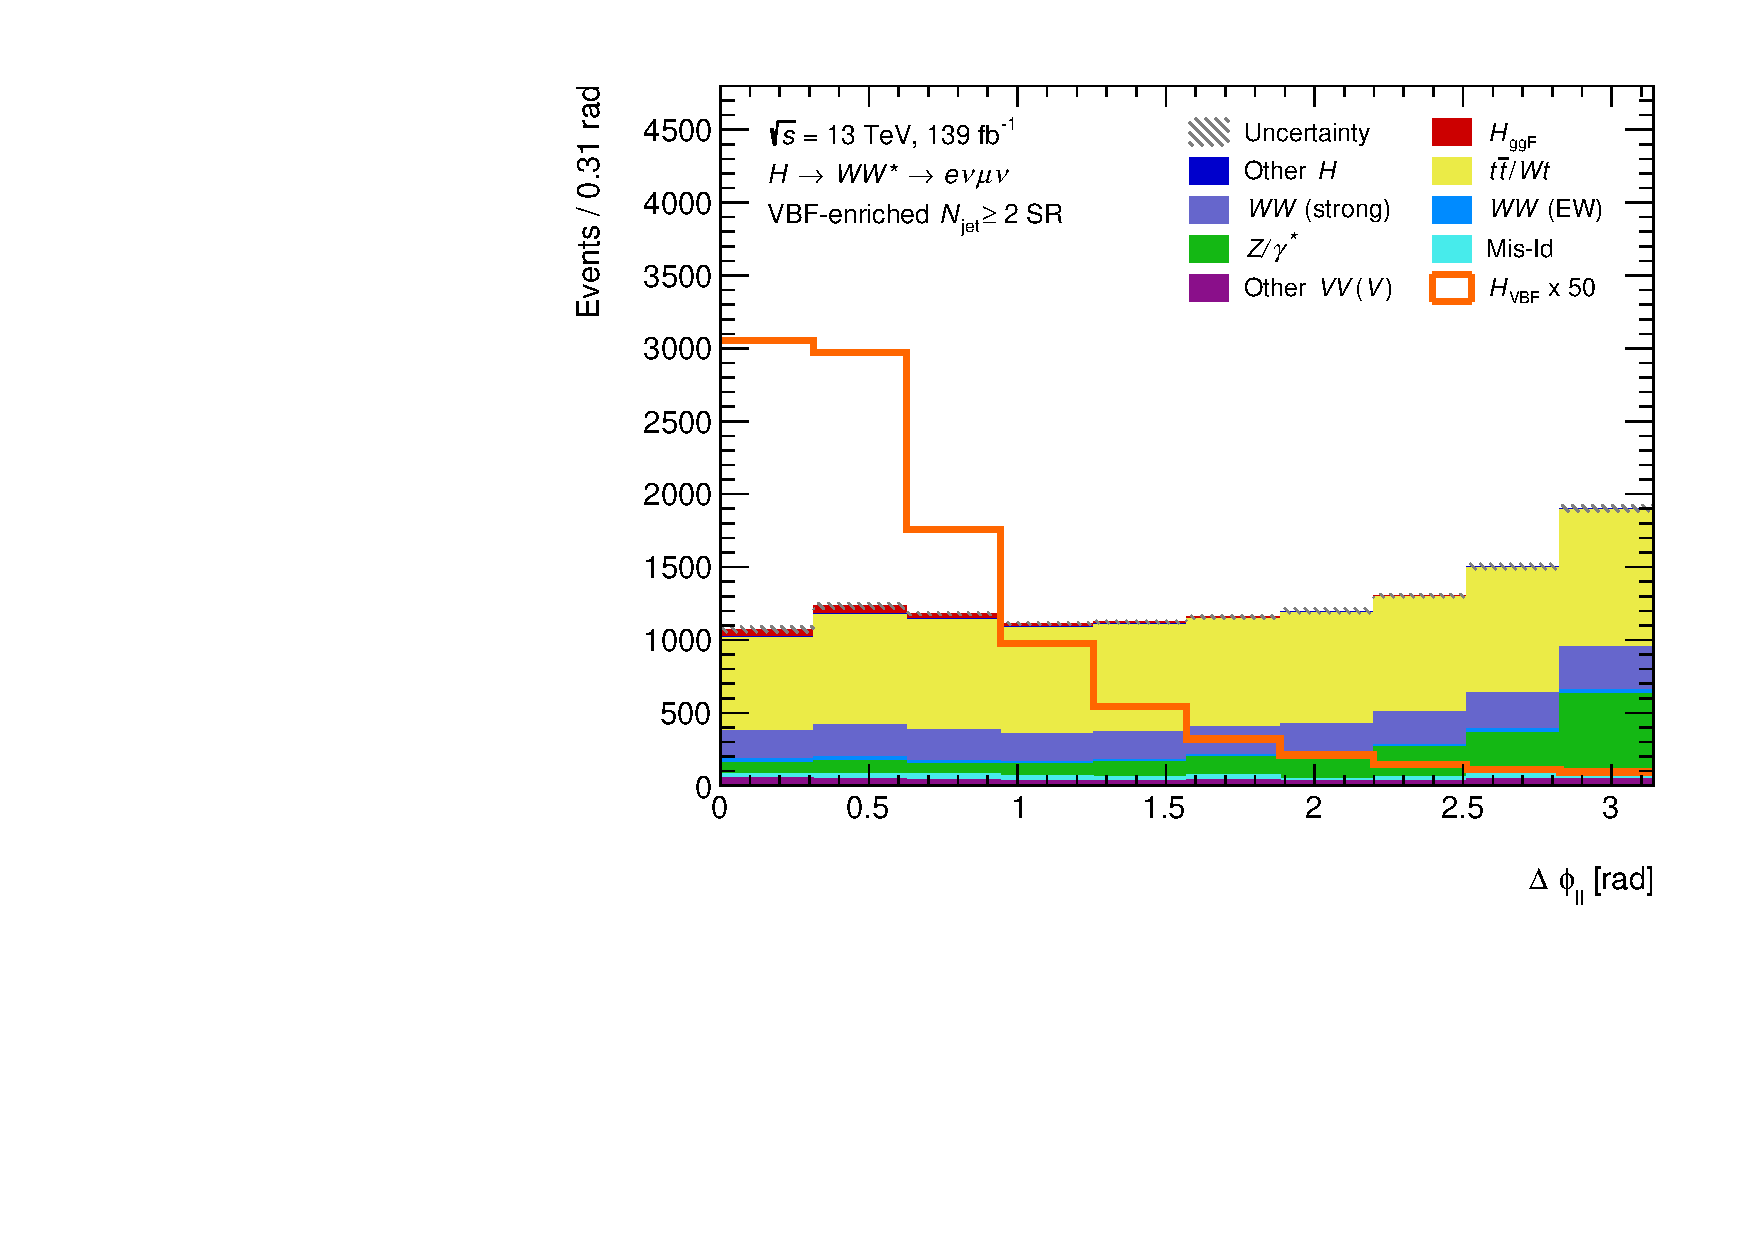
\includegraphics[width=0.32\textwidth]{figures/hww/dnn/blinded/run2-emme-CutVBF_SR-DPhill-lin.pdf} \hfill
            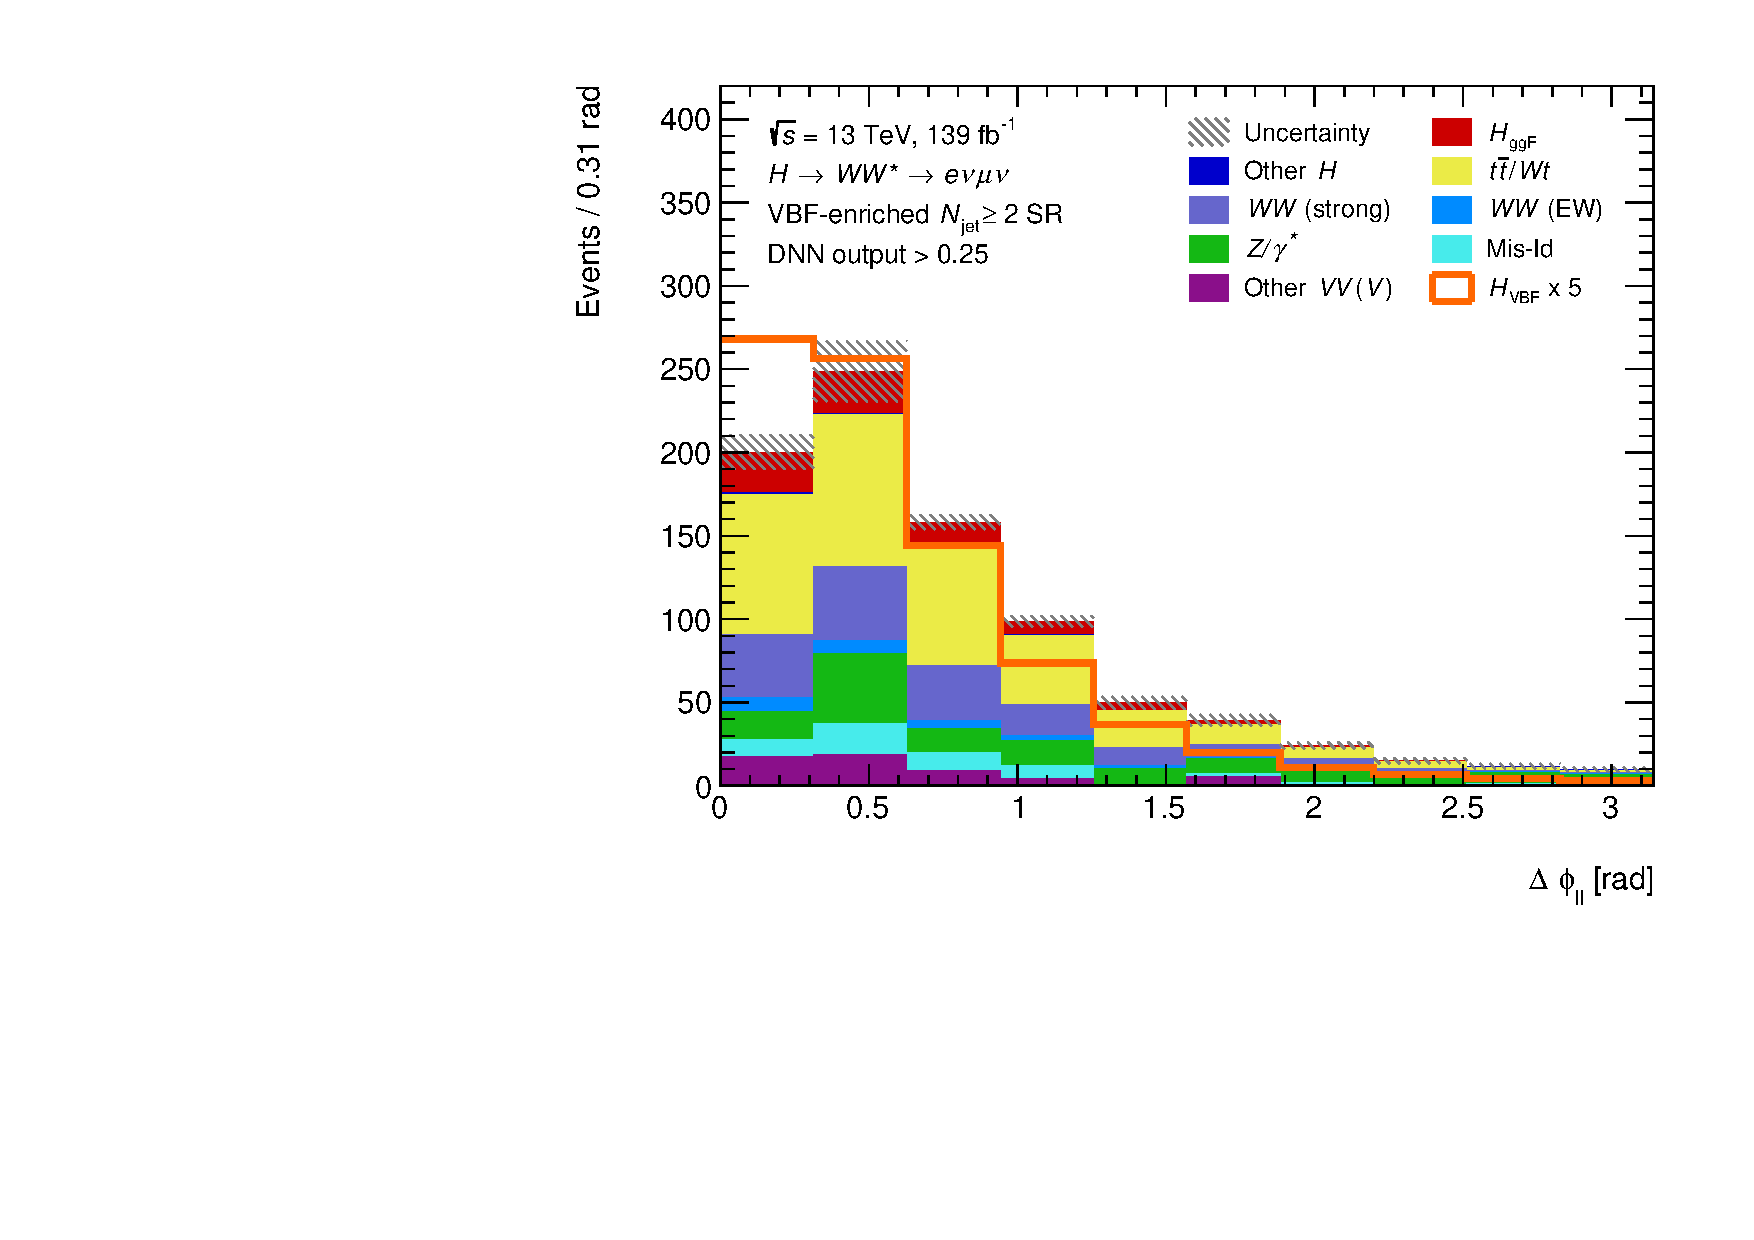
\includegraphics[width=0.32\textwidth]{figures/hww/dnn/blinded/run2-emme-CutVBFSR_DNN25-DPhill-lin.pdf} \hfill
            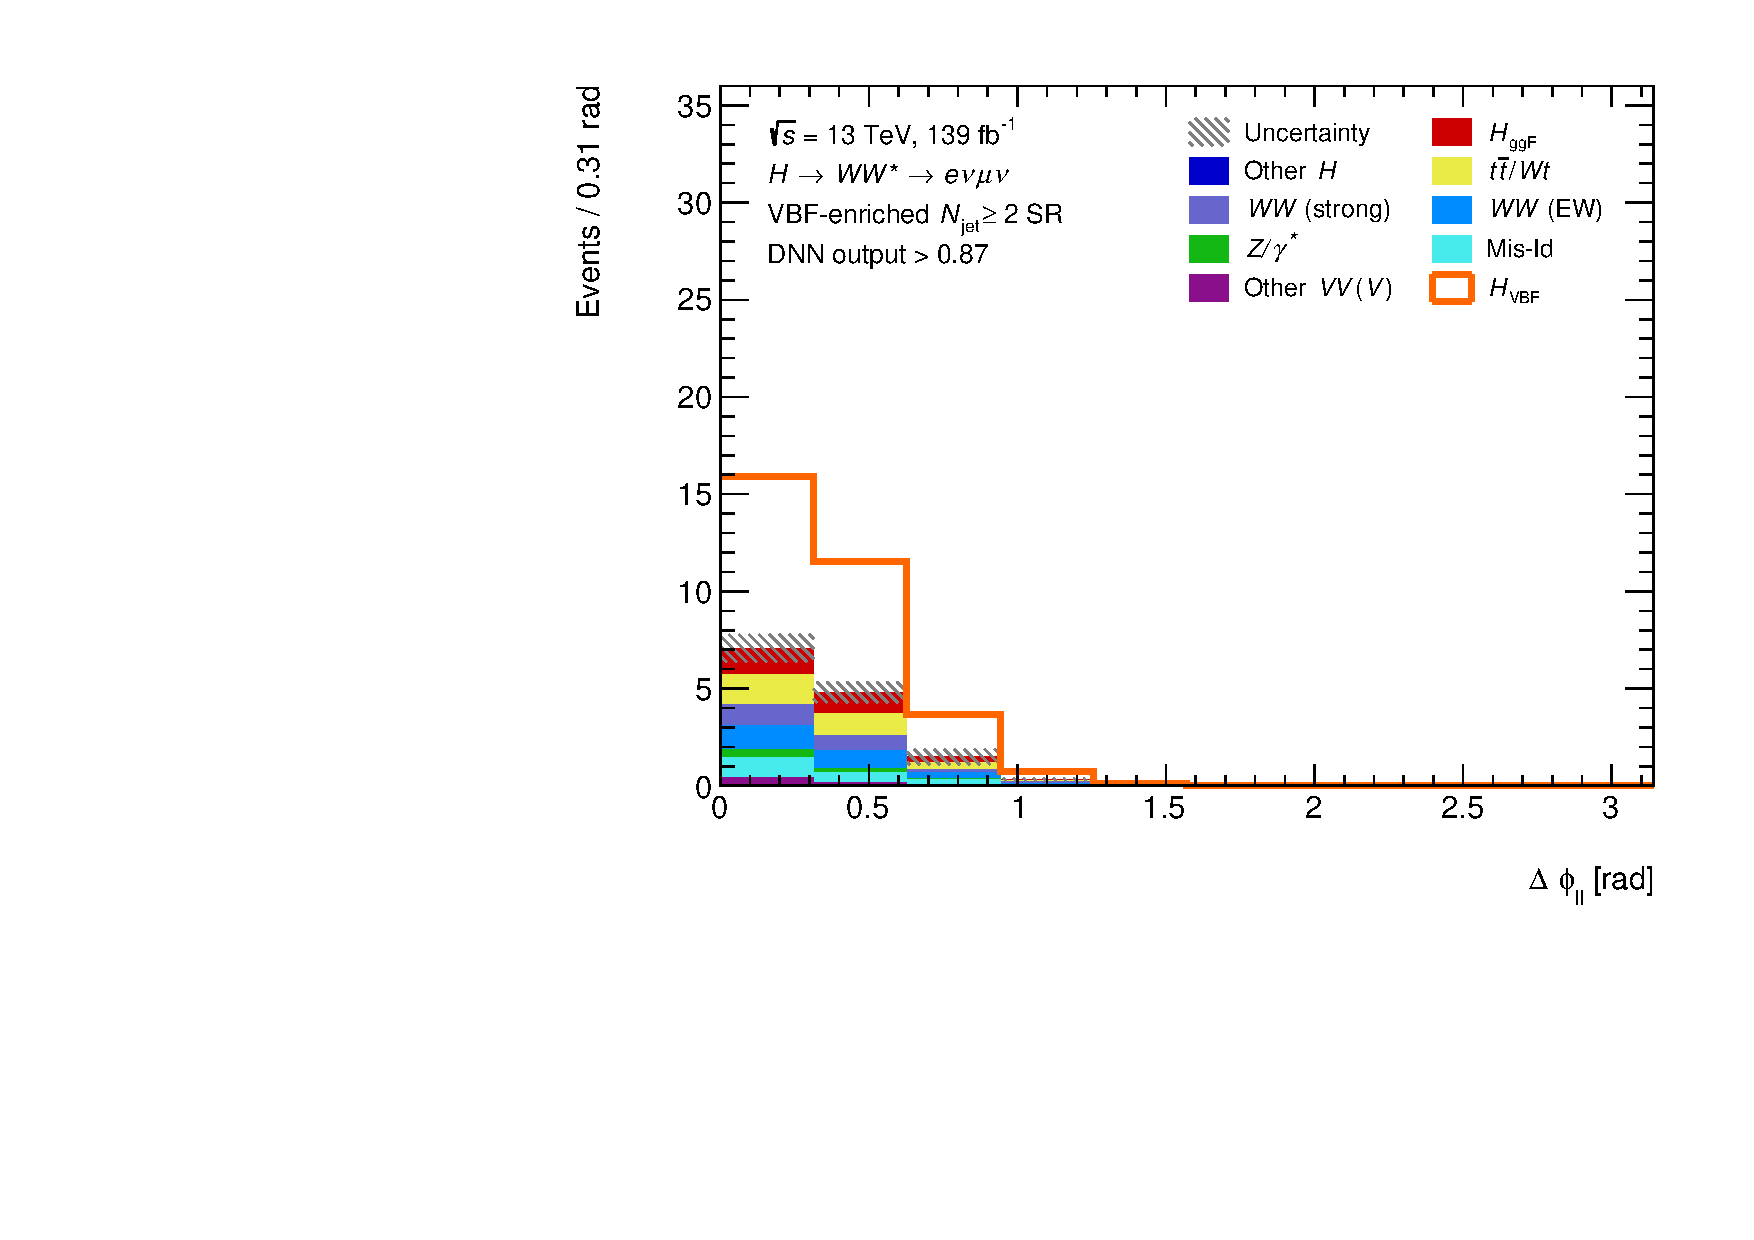
\includegraphics[width=0.32\textwidth]{figures/hww/dnn/blinded/run2-emme-CutVBFSR_DNN87-DPhill-lin.pdf}
        } \\
        \subfloat[$\mll$]{
            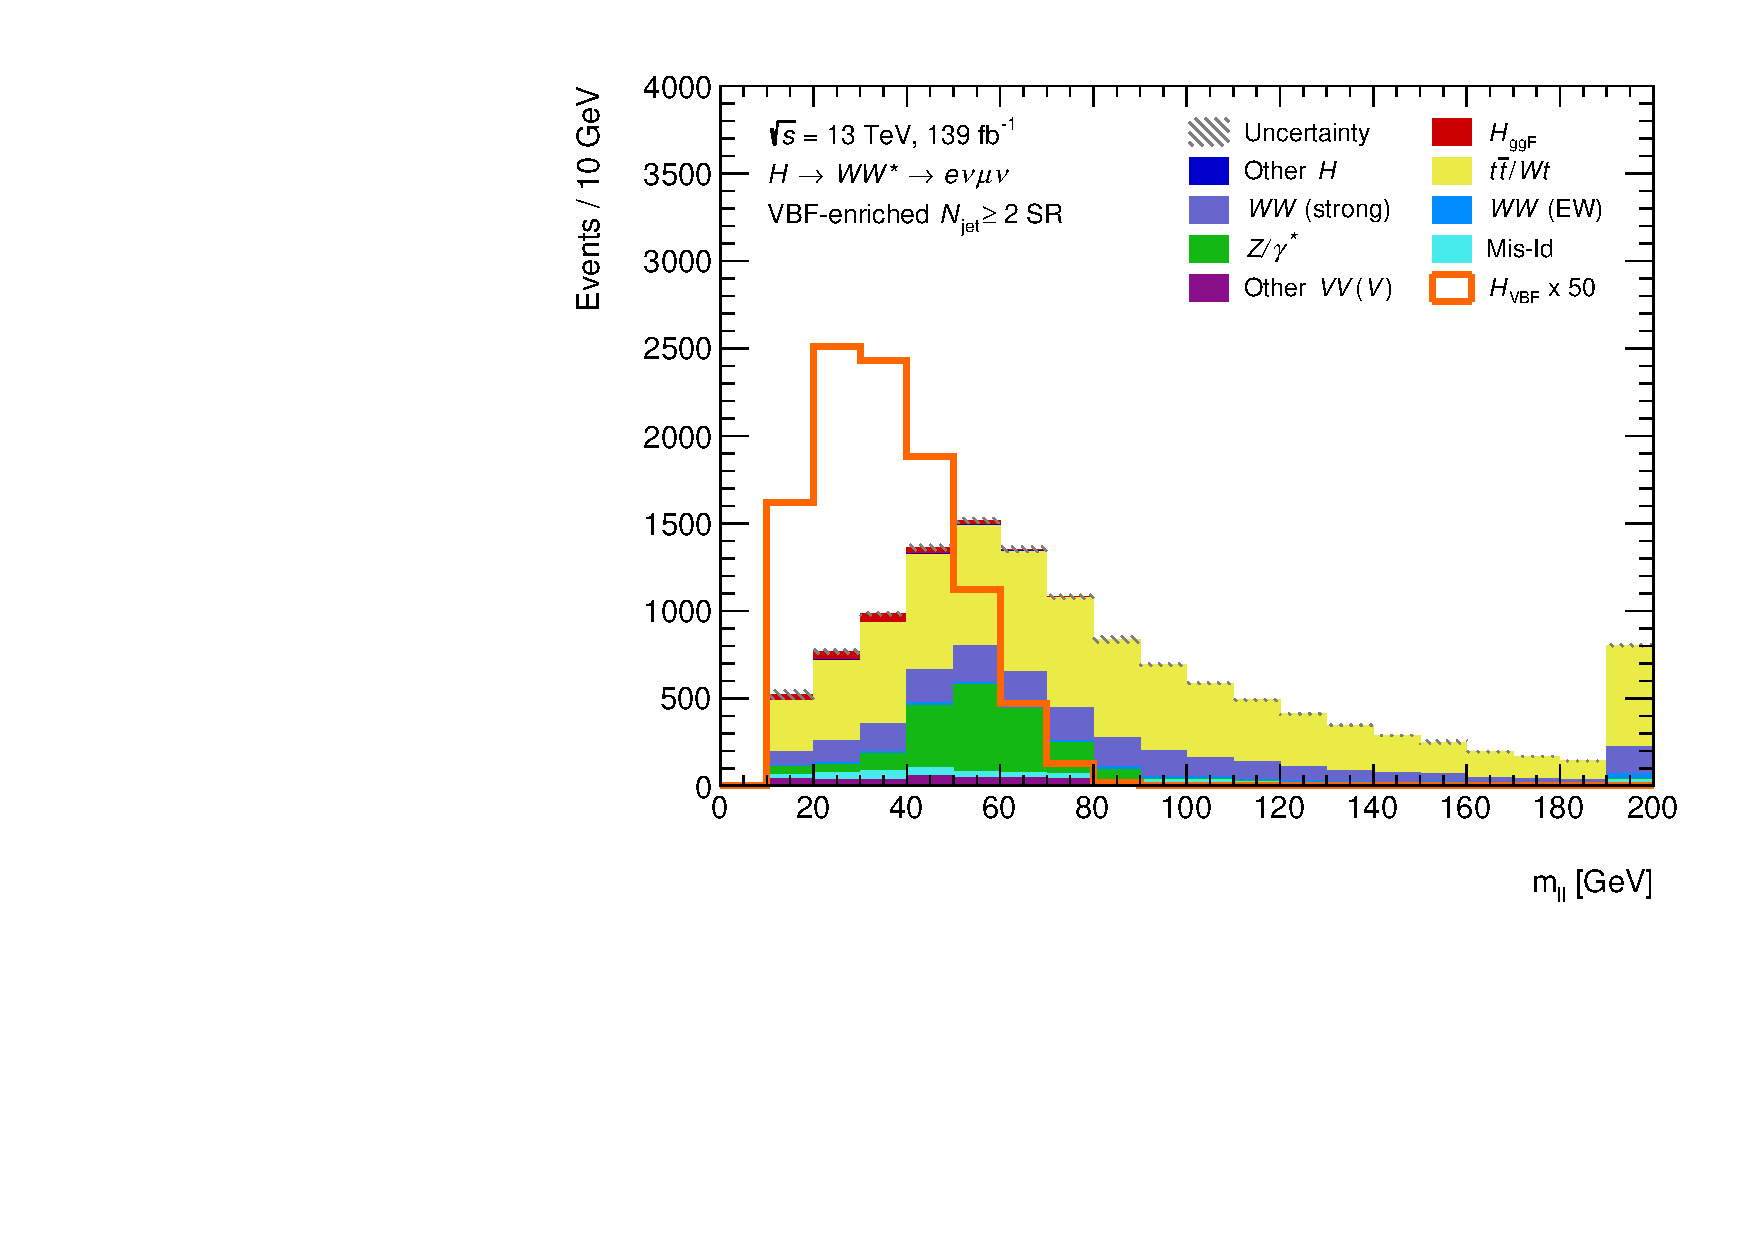
\includegraphics[width=0.32\textwidth]{figures/hww/dnn/blinded/run2-emme-CutVBF_SR-Mll-lin.pdf}
            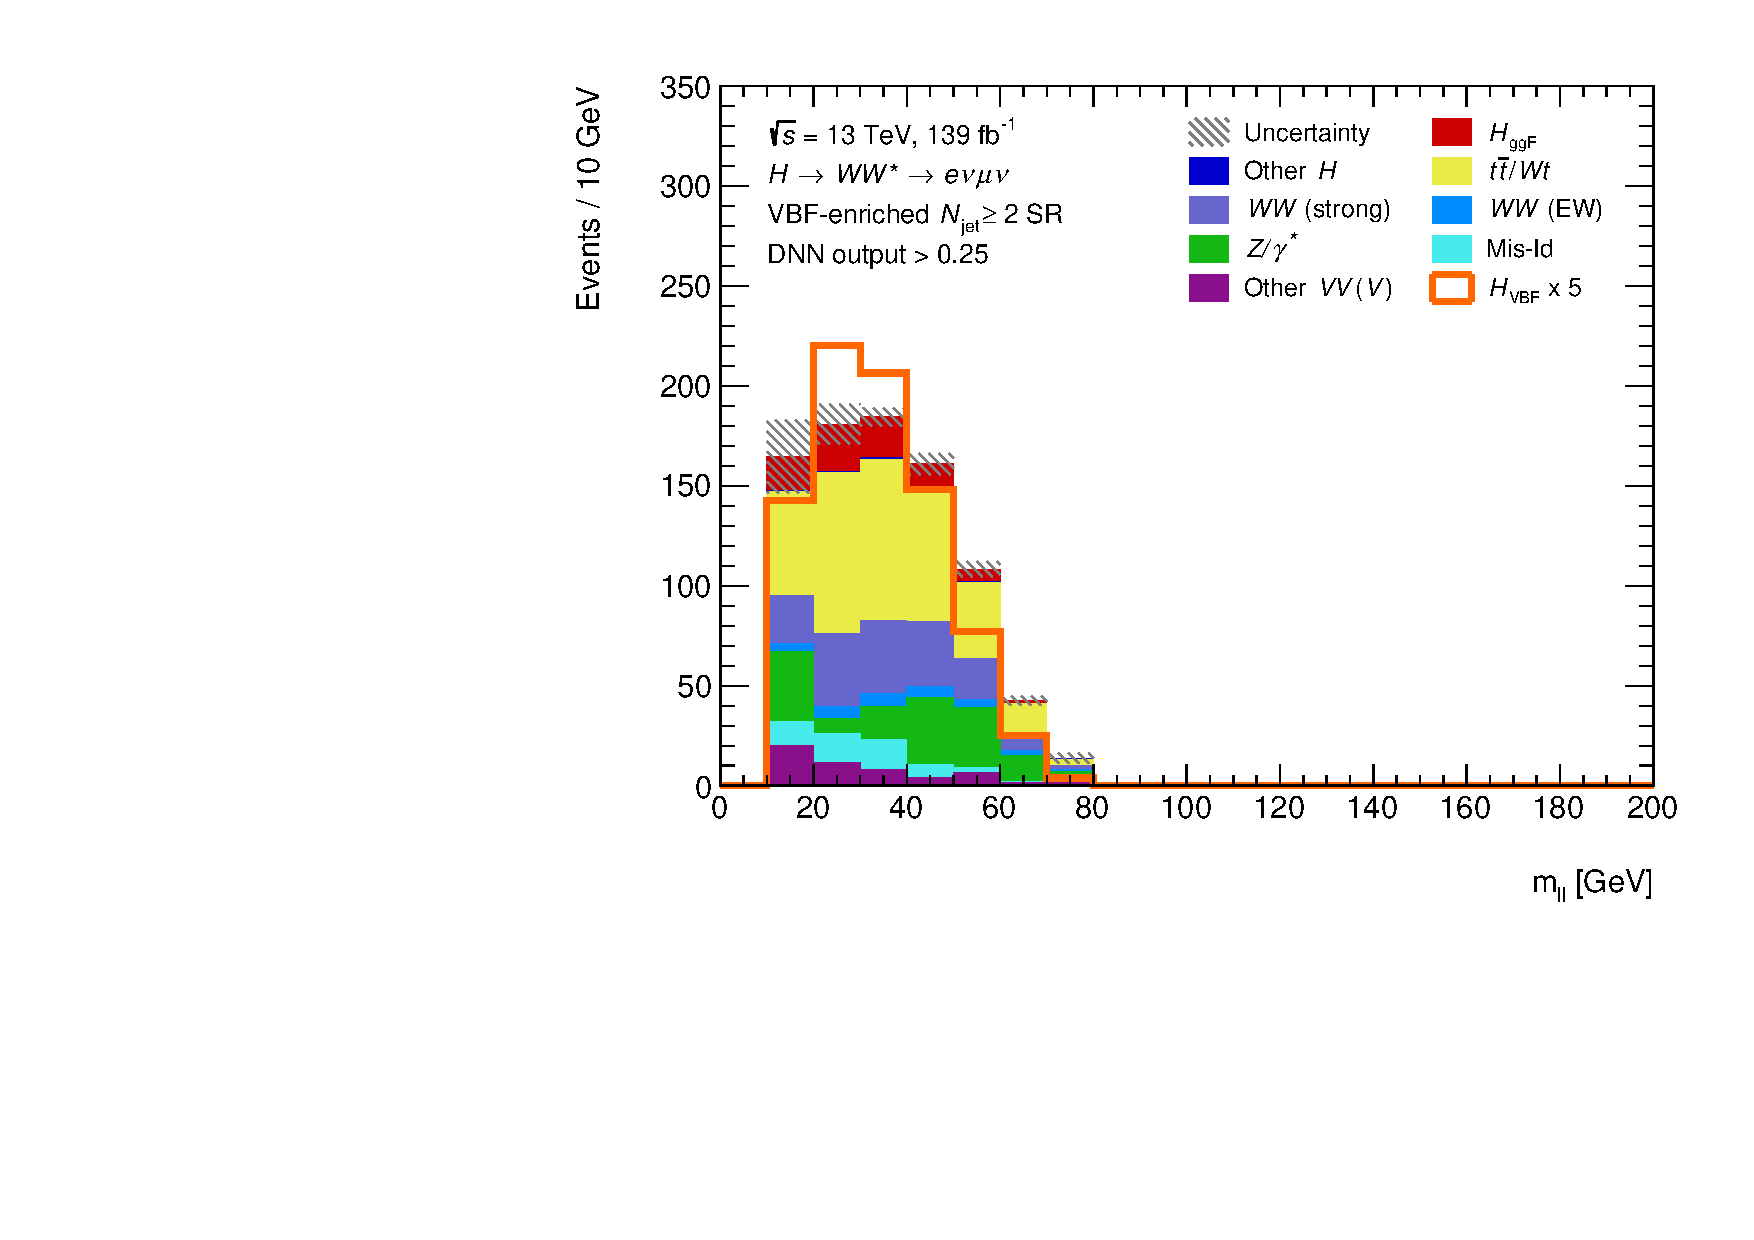
\includegraphics[width=0.32\textwidth]{figures/hww/dnn/blinded/run2-emme-CutVBFSR_DNN25-Mll-lin.pdf}
            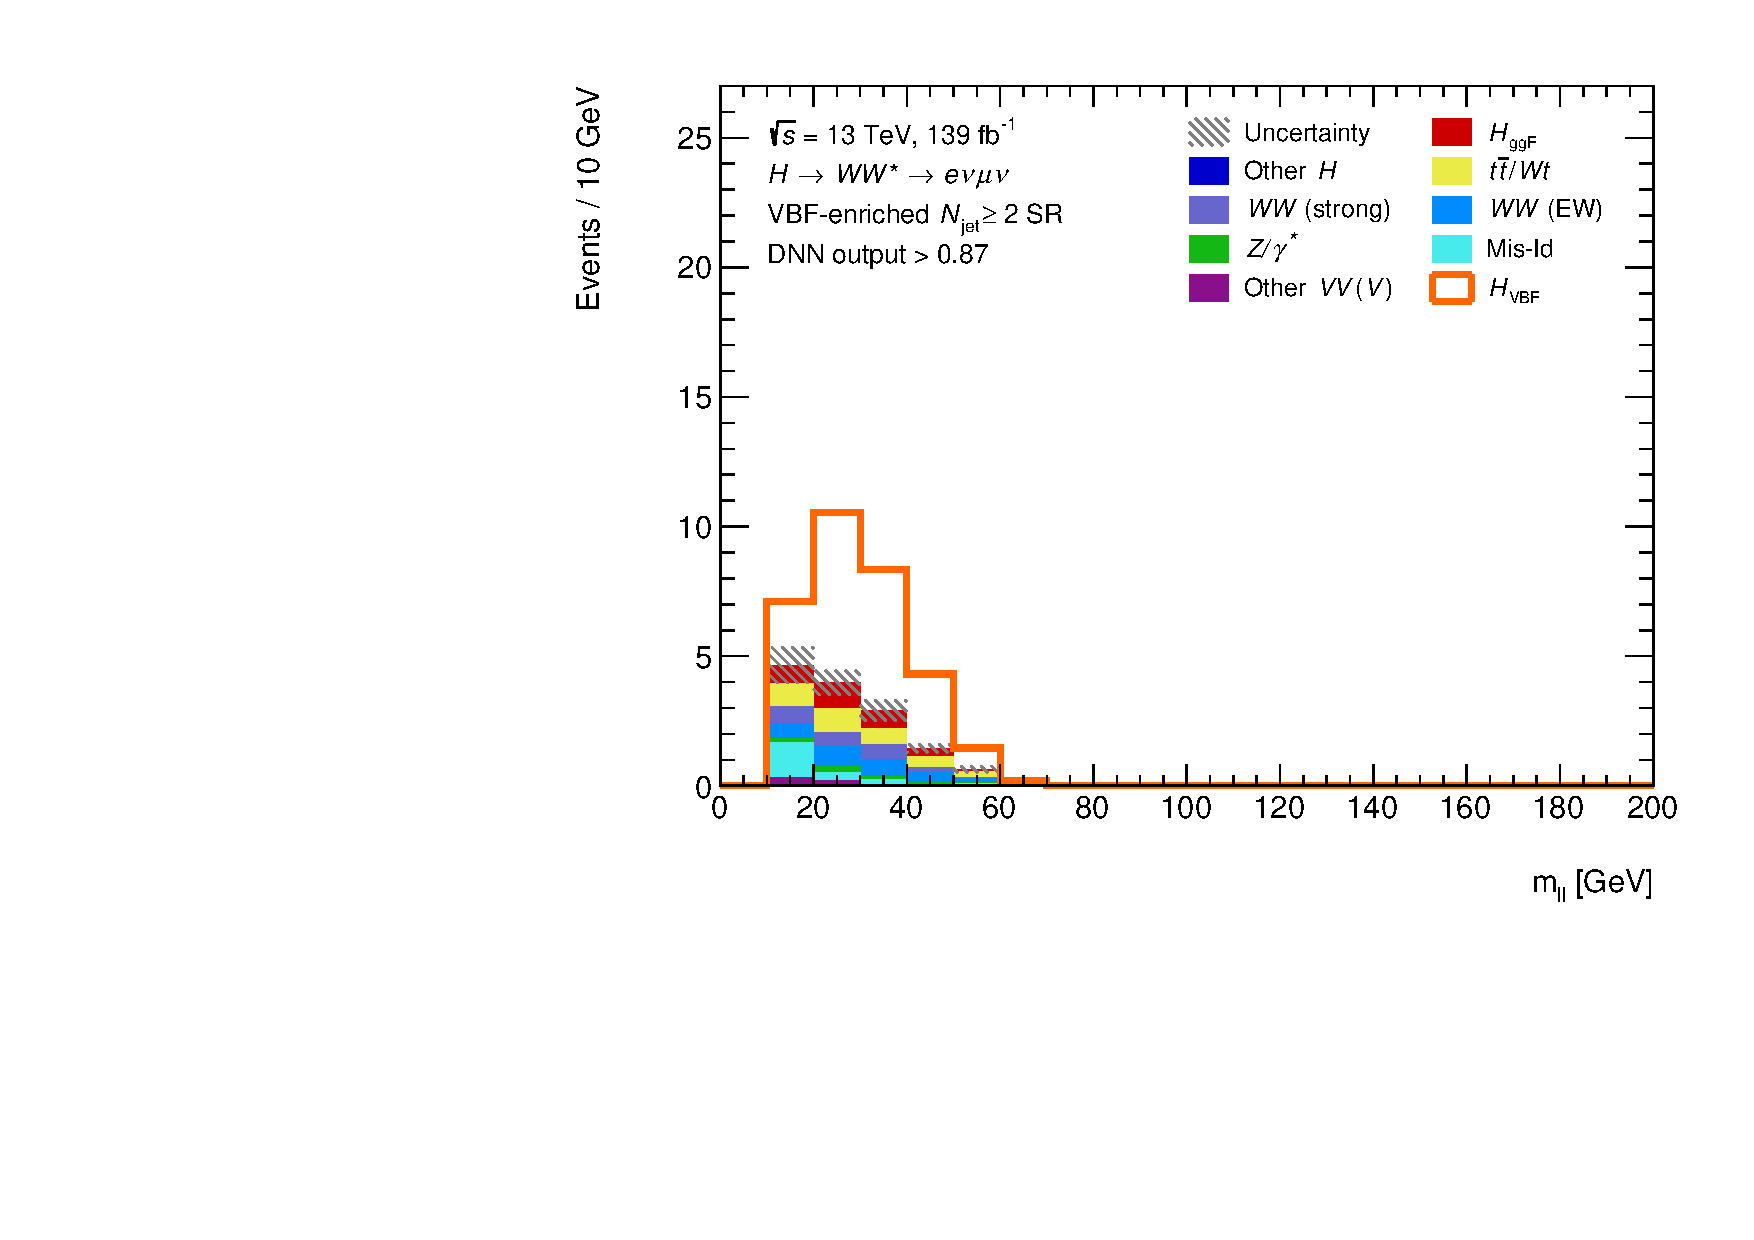
\includegraphics[width=0.32\textwidth]{figures/hww/dnn/blinded/run2-emme-CutVBFSR_DNN87-Mll-lin.pdf}
        } \\
        \subfloat[$\mT$]{
            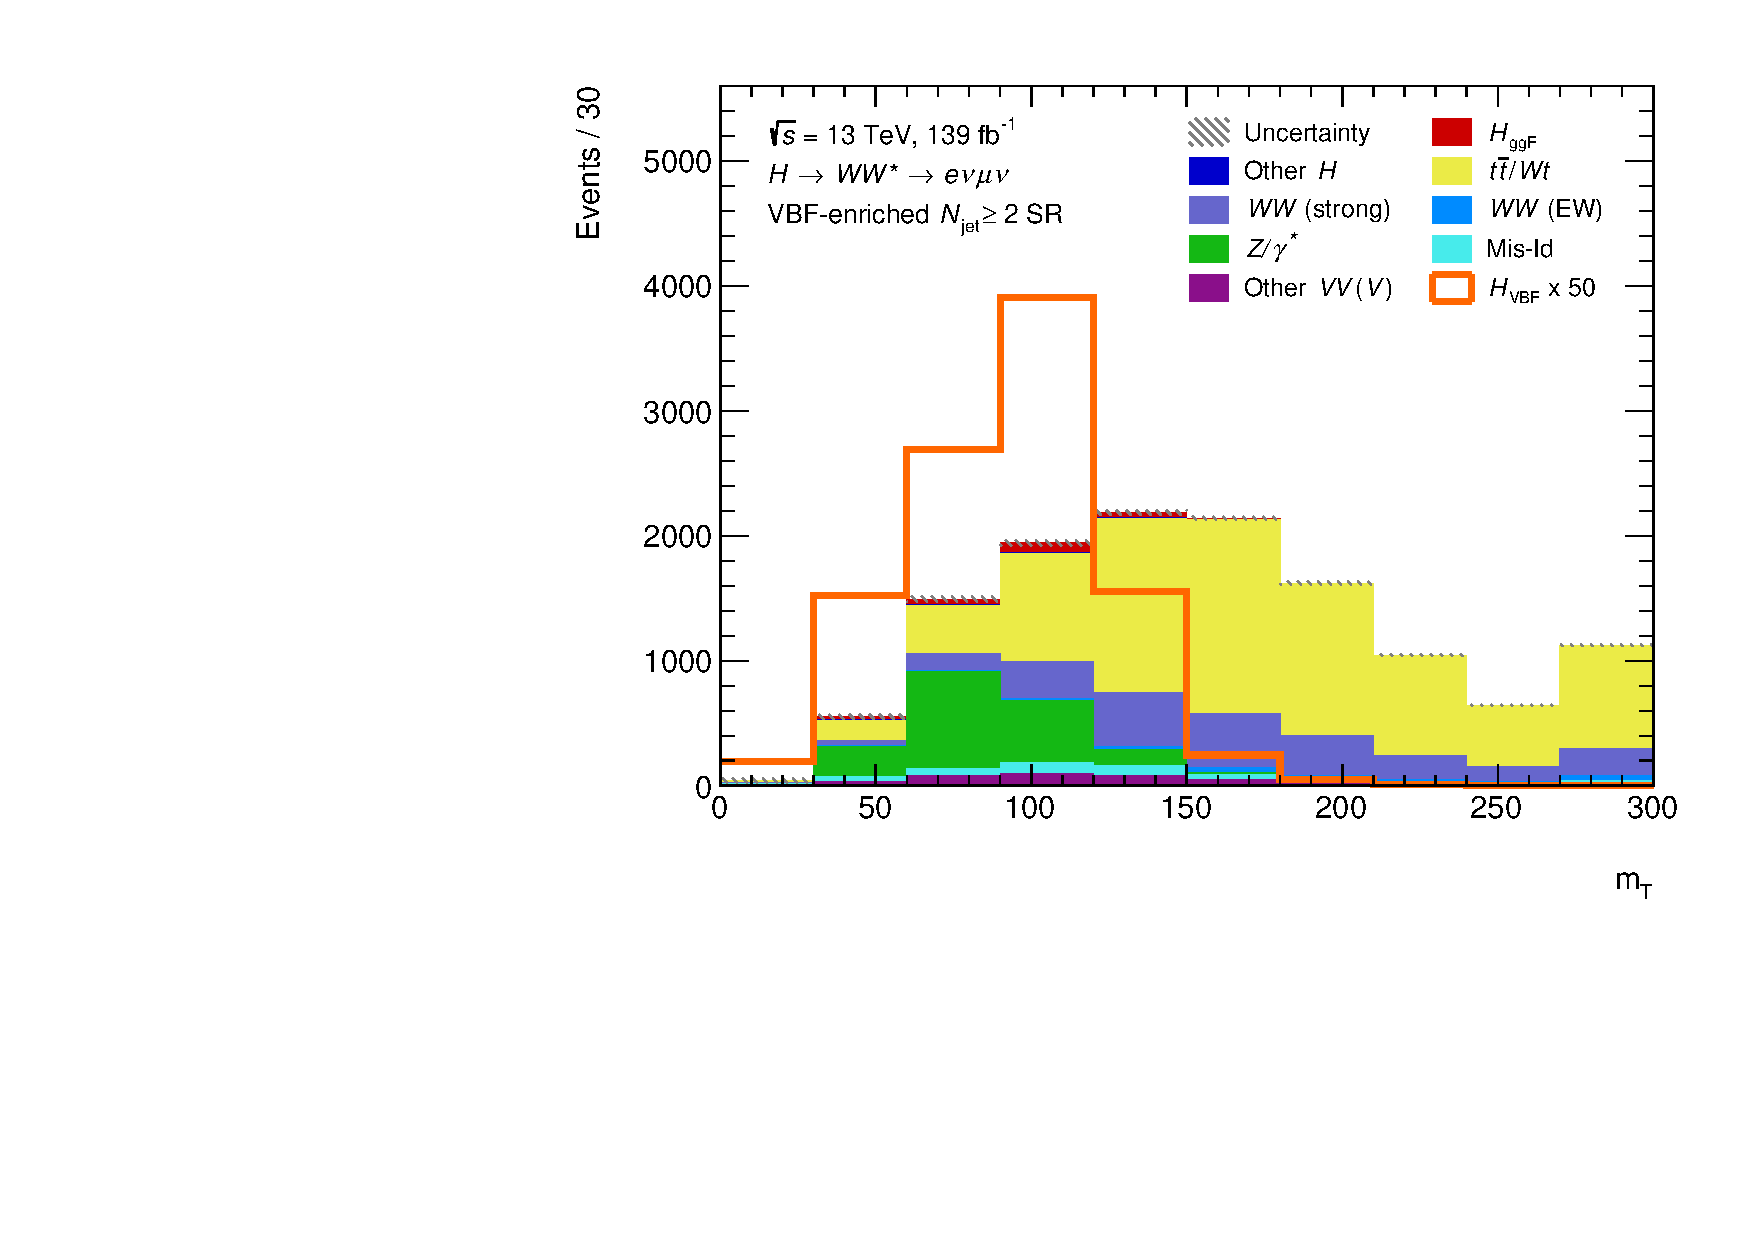
\includegraphics[width=0.32\textwidth]{figures/hww/dnn/blinded/run2-emme-CutVBF_SR-MT-lin.pdf} \hfill
            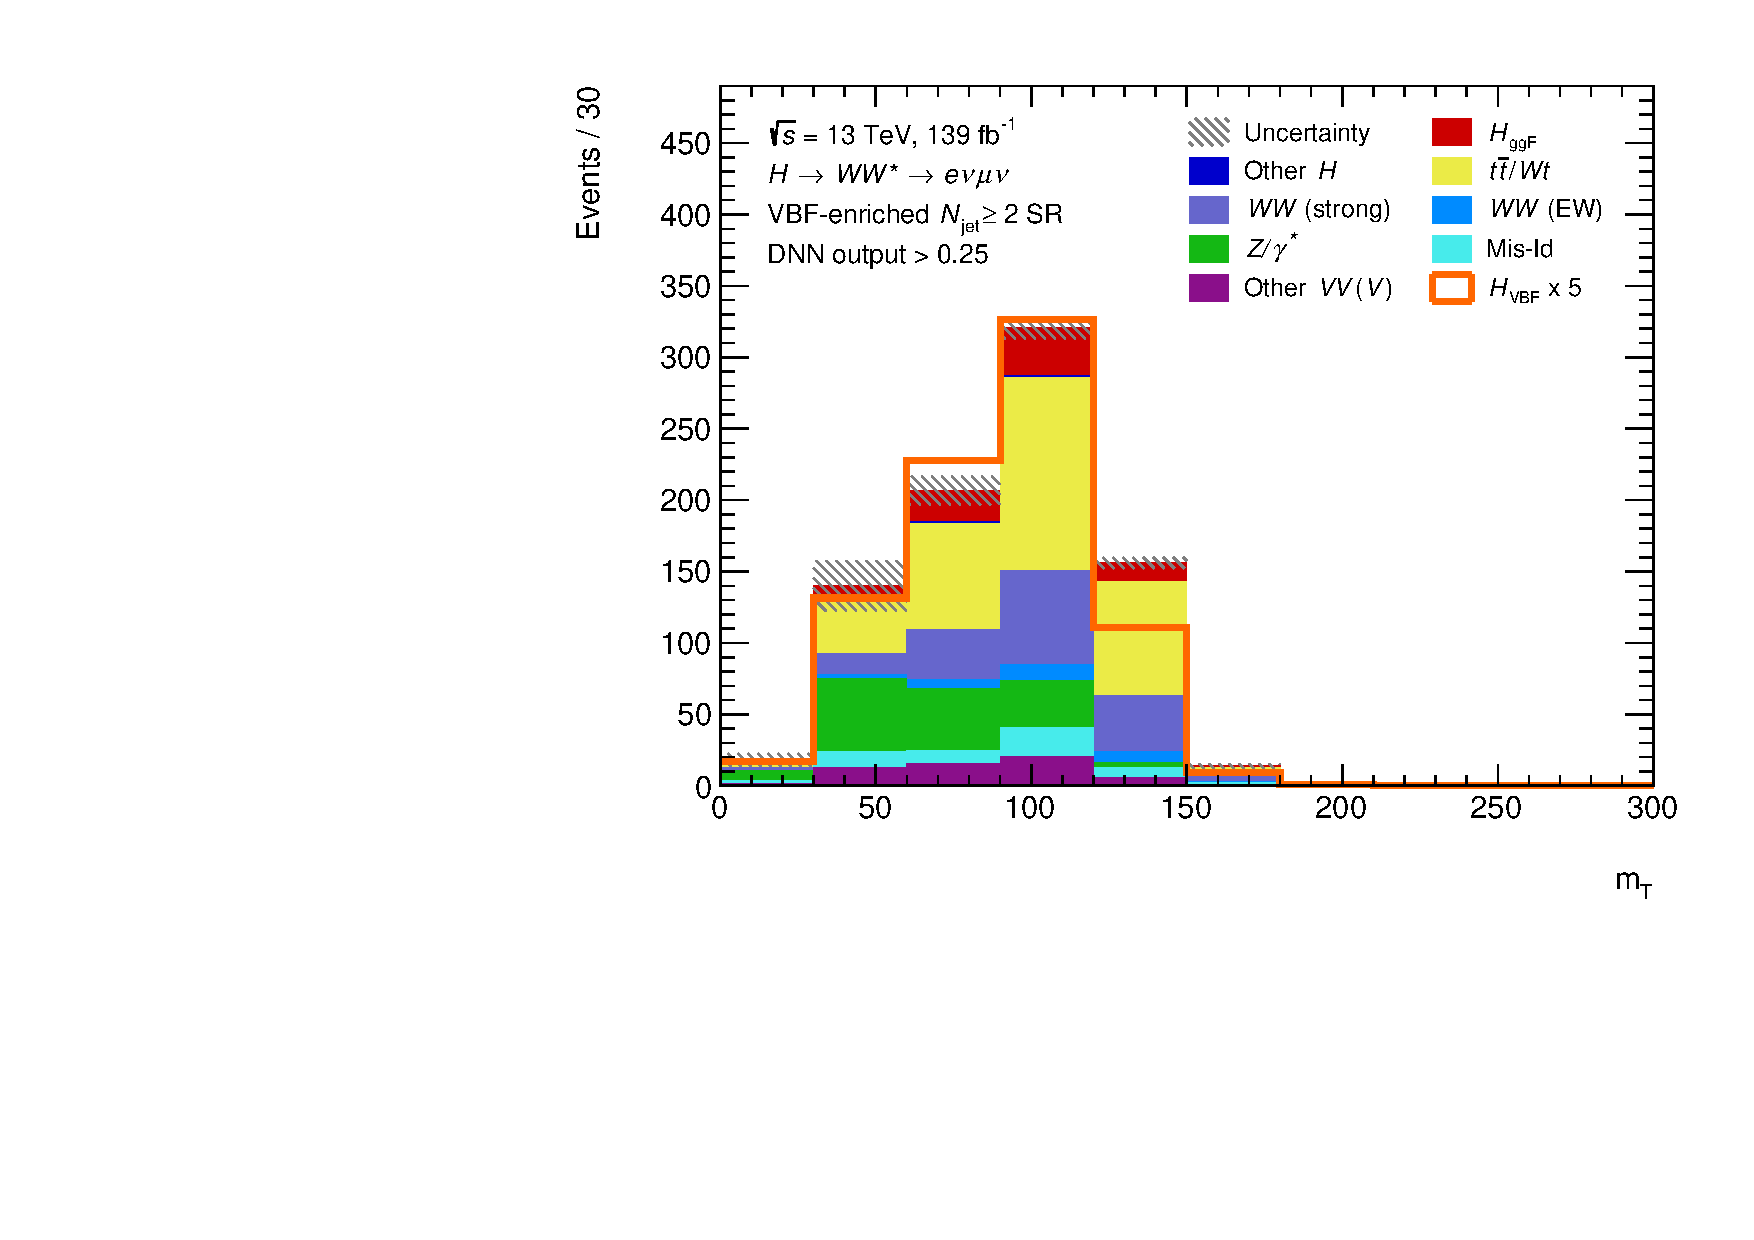
\includegraphics[width=0.32\textwidth]{figures/hww/dnn/blinded/run2-emme-CutVBFSR_DNN25-MT-lin.pdf} \hfill
            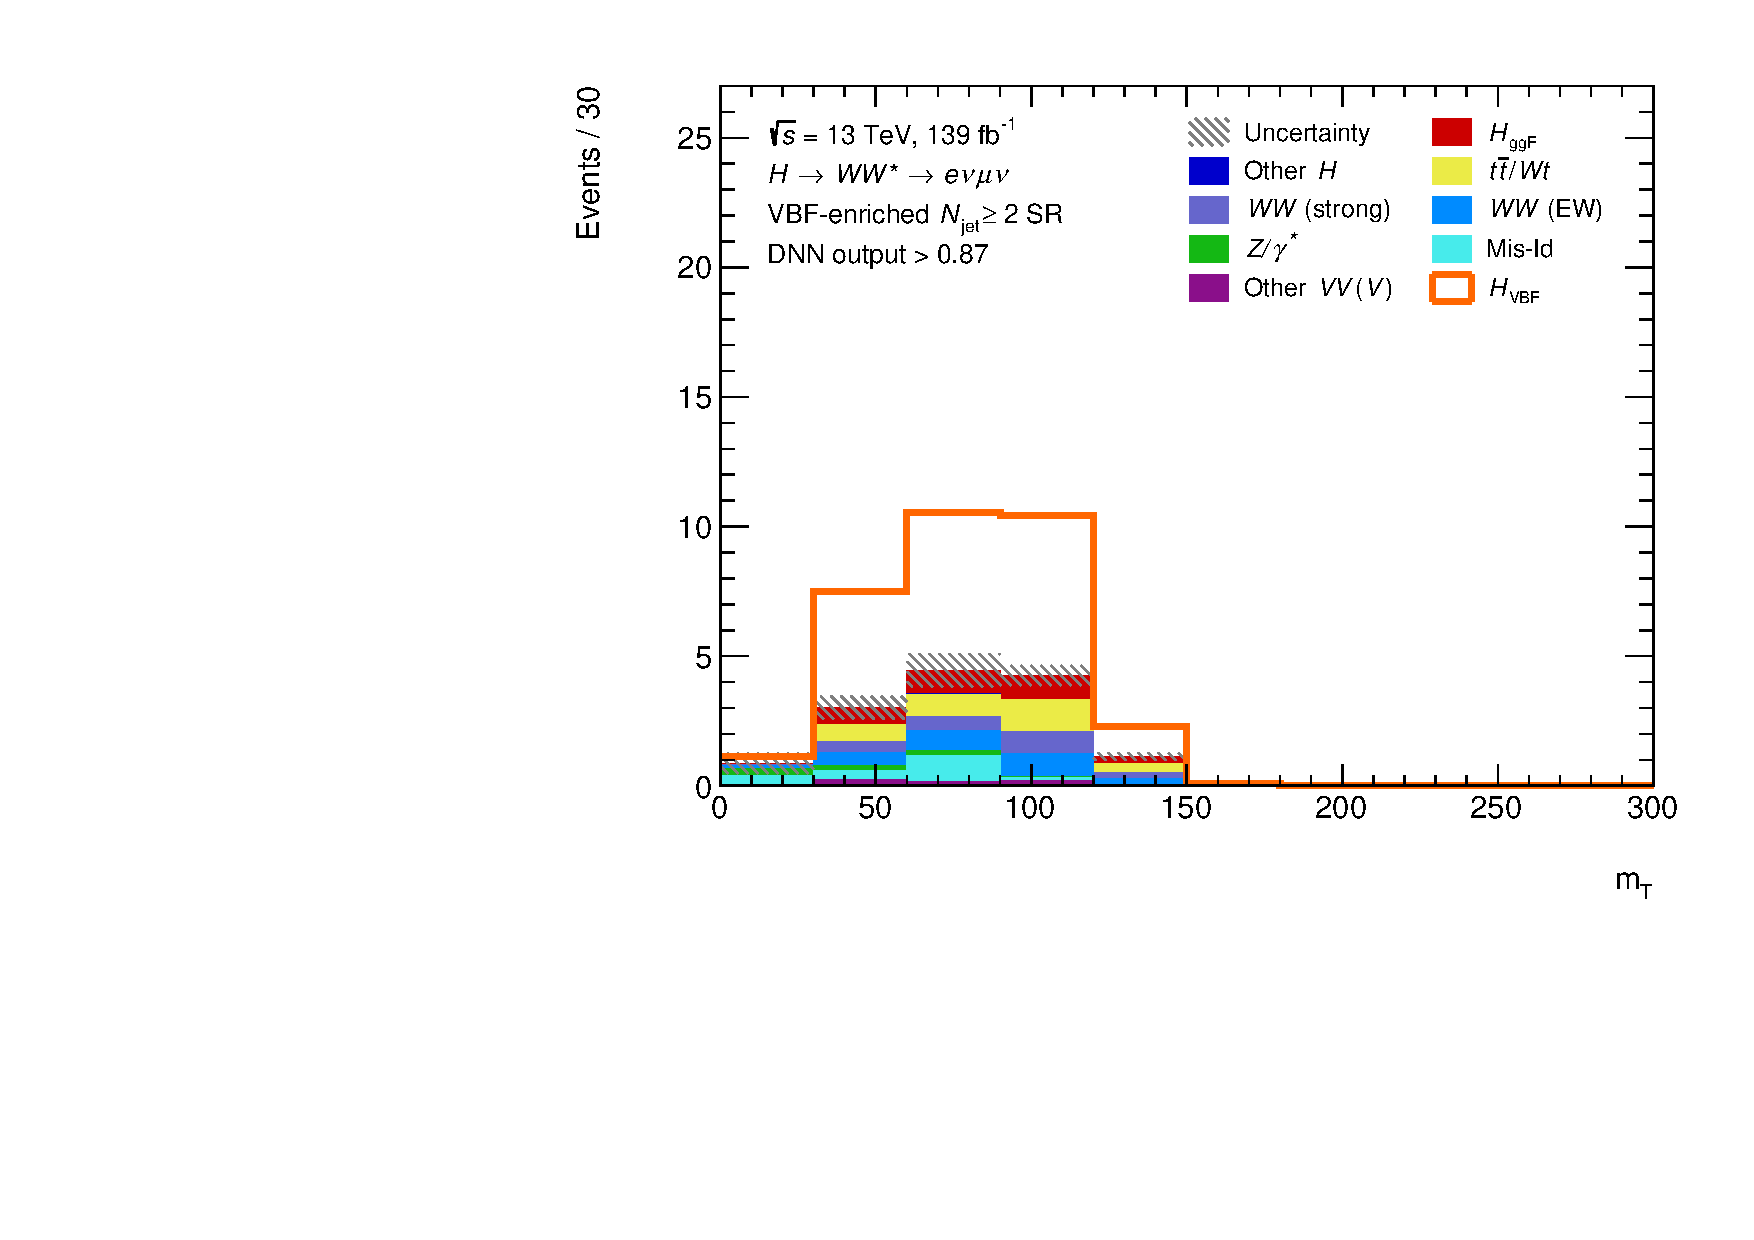
\includegraphics[width=0.32\textwidth]{figures/hww/dnn/blinded/run2-emme-CutVBFSR_DNN87-MT-lin.pdf}
        }
        {\caption[Distributions of $\dphill$, $\mll$, $\mT$ in the VBF \TwoJet signal region.]{Distributions of $\dphill$, $\mll$, $\mT$ in the VBF \TwoJet signal region.
                Each row corresponds to one variable with different selections made on the DNN output as indicated in the figure. The solid orange line shows the expected VBF signal scaled by a factor of (left) 50, (center) 5, and (right) without any scaling.
                \label{app:fig:dnn-inputs-hwwdecay} }}
    \end{figure}



    \begin{figure}[h]
        \centering
        \subfloat[$\pttot$]{
            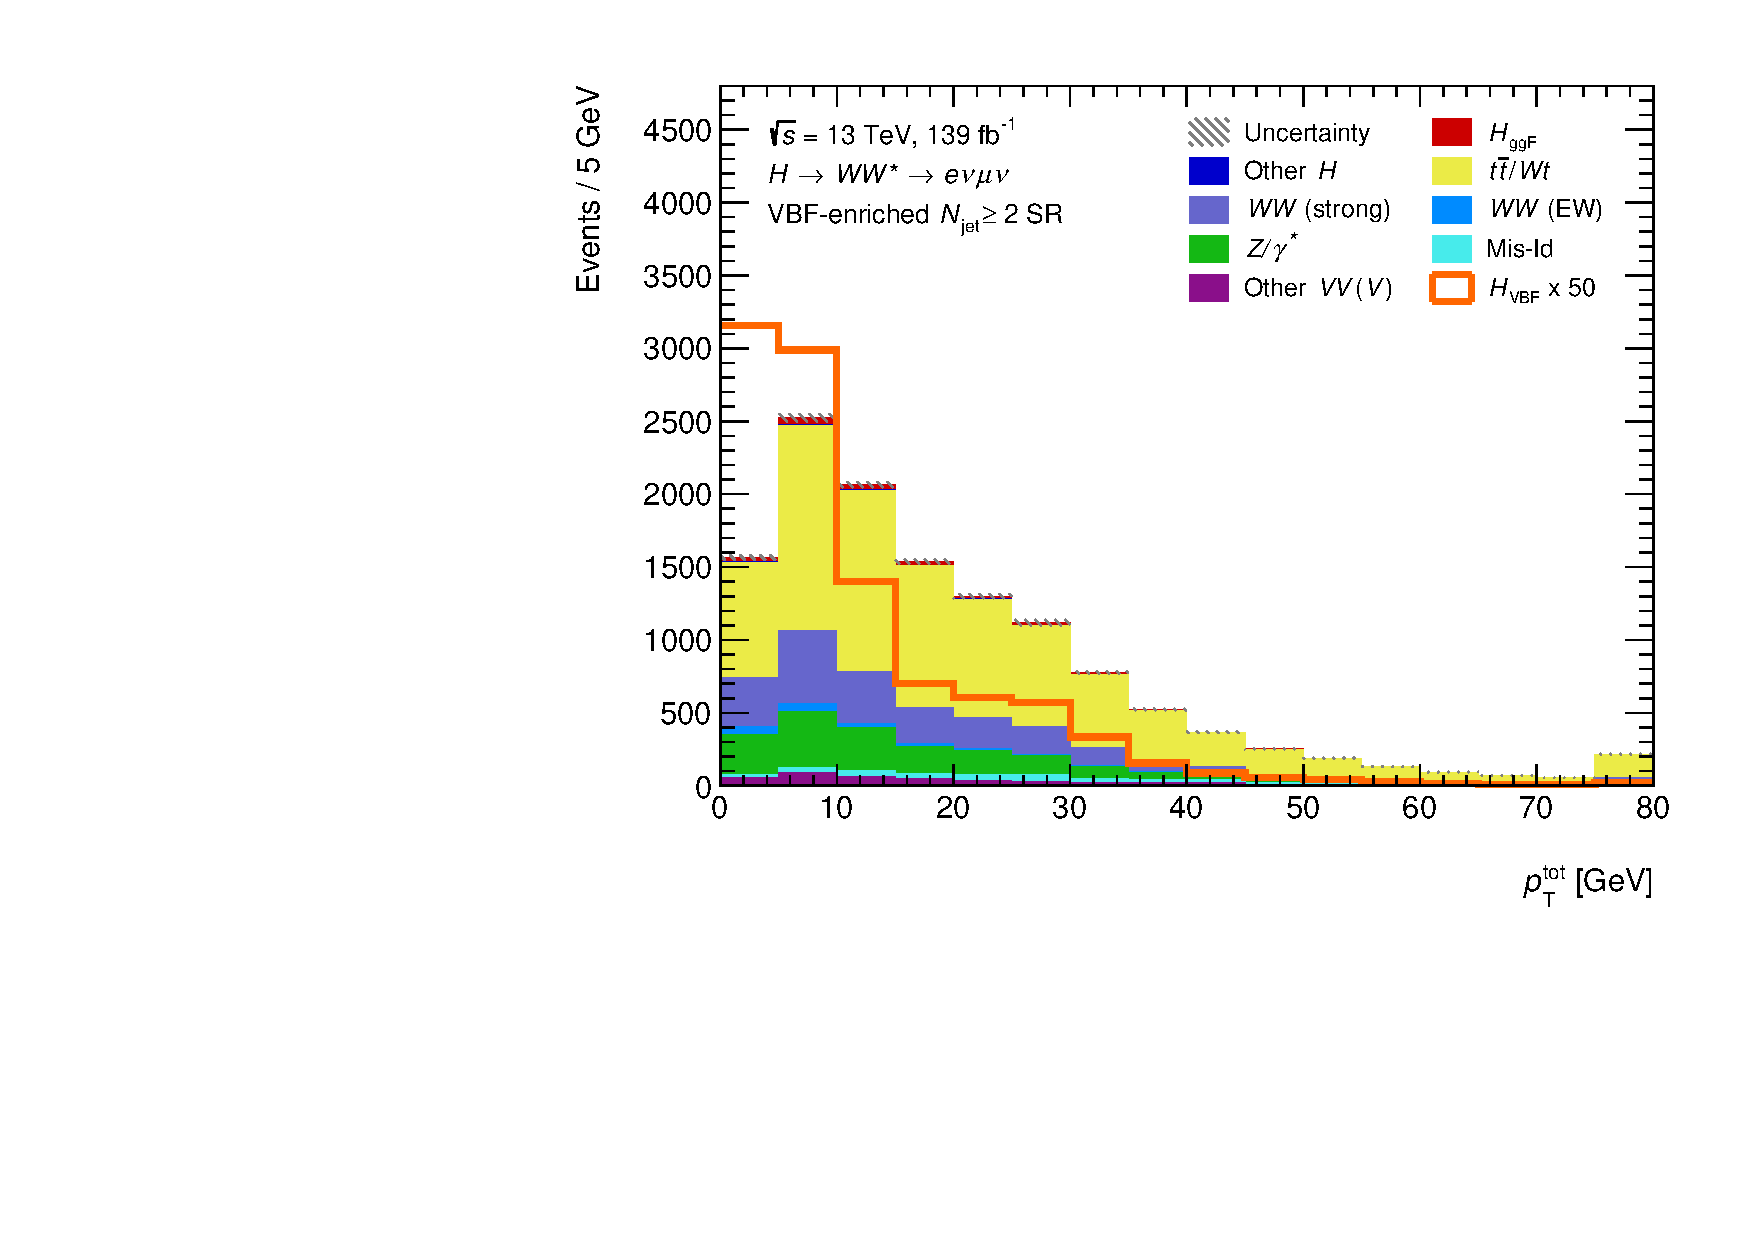
\includegraphics[width=0.32\textwidth]{figures/hww/dnn/blinded/run2-emme-CutVBF_SR-PtTot-lin.pdf} \hfill
            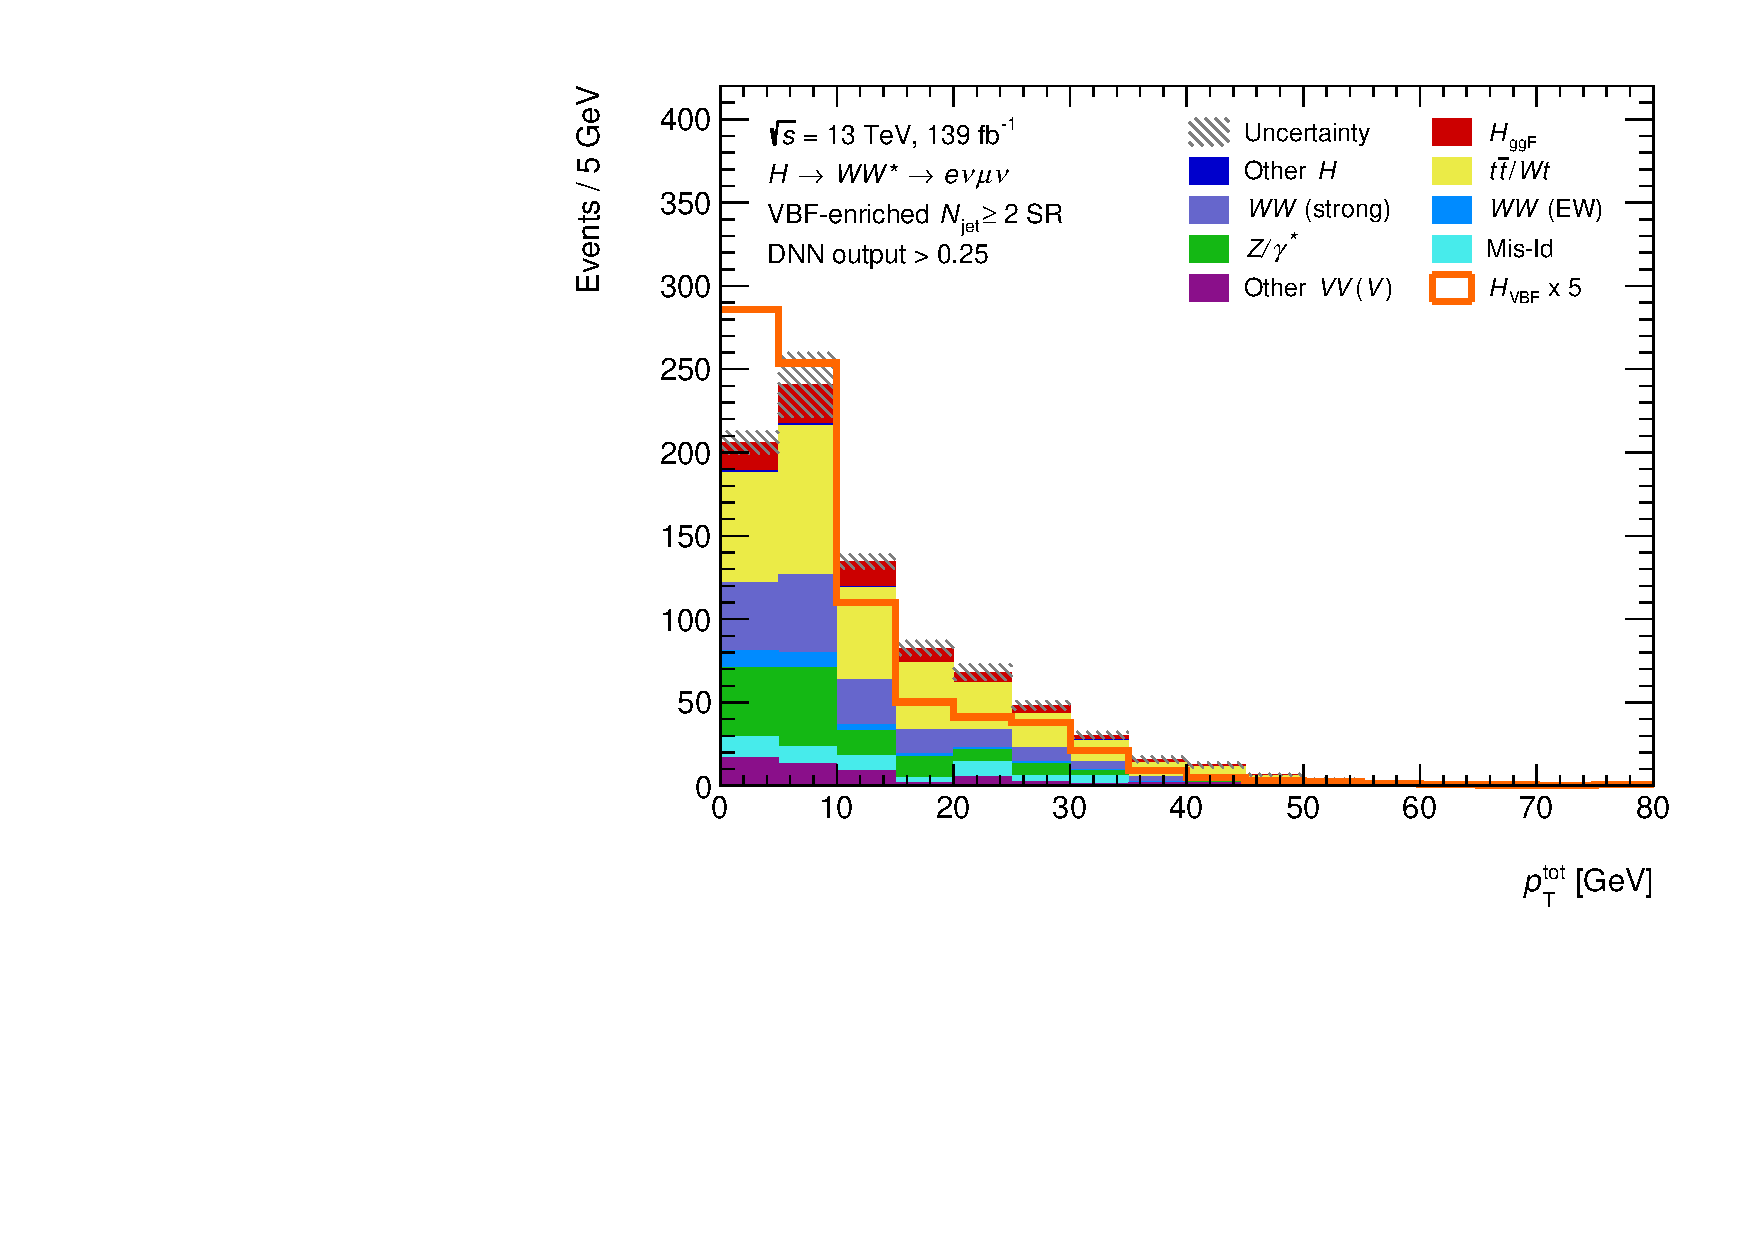
\includegraphics[width=0.32\textwidth]{figures/hww/dnn/blinded/run2-emme-CutVBFSR_DNN25-PtTot-lin.pdf} \hfill
            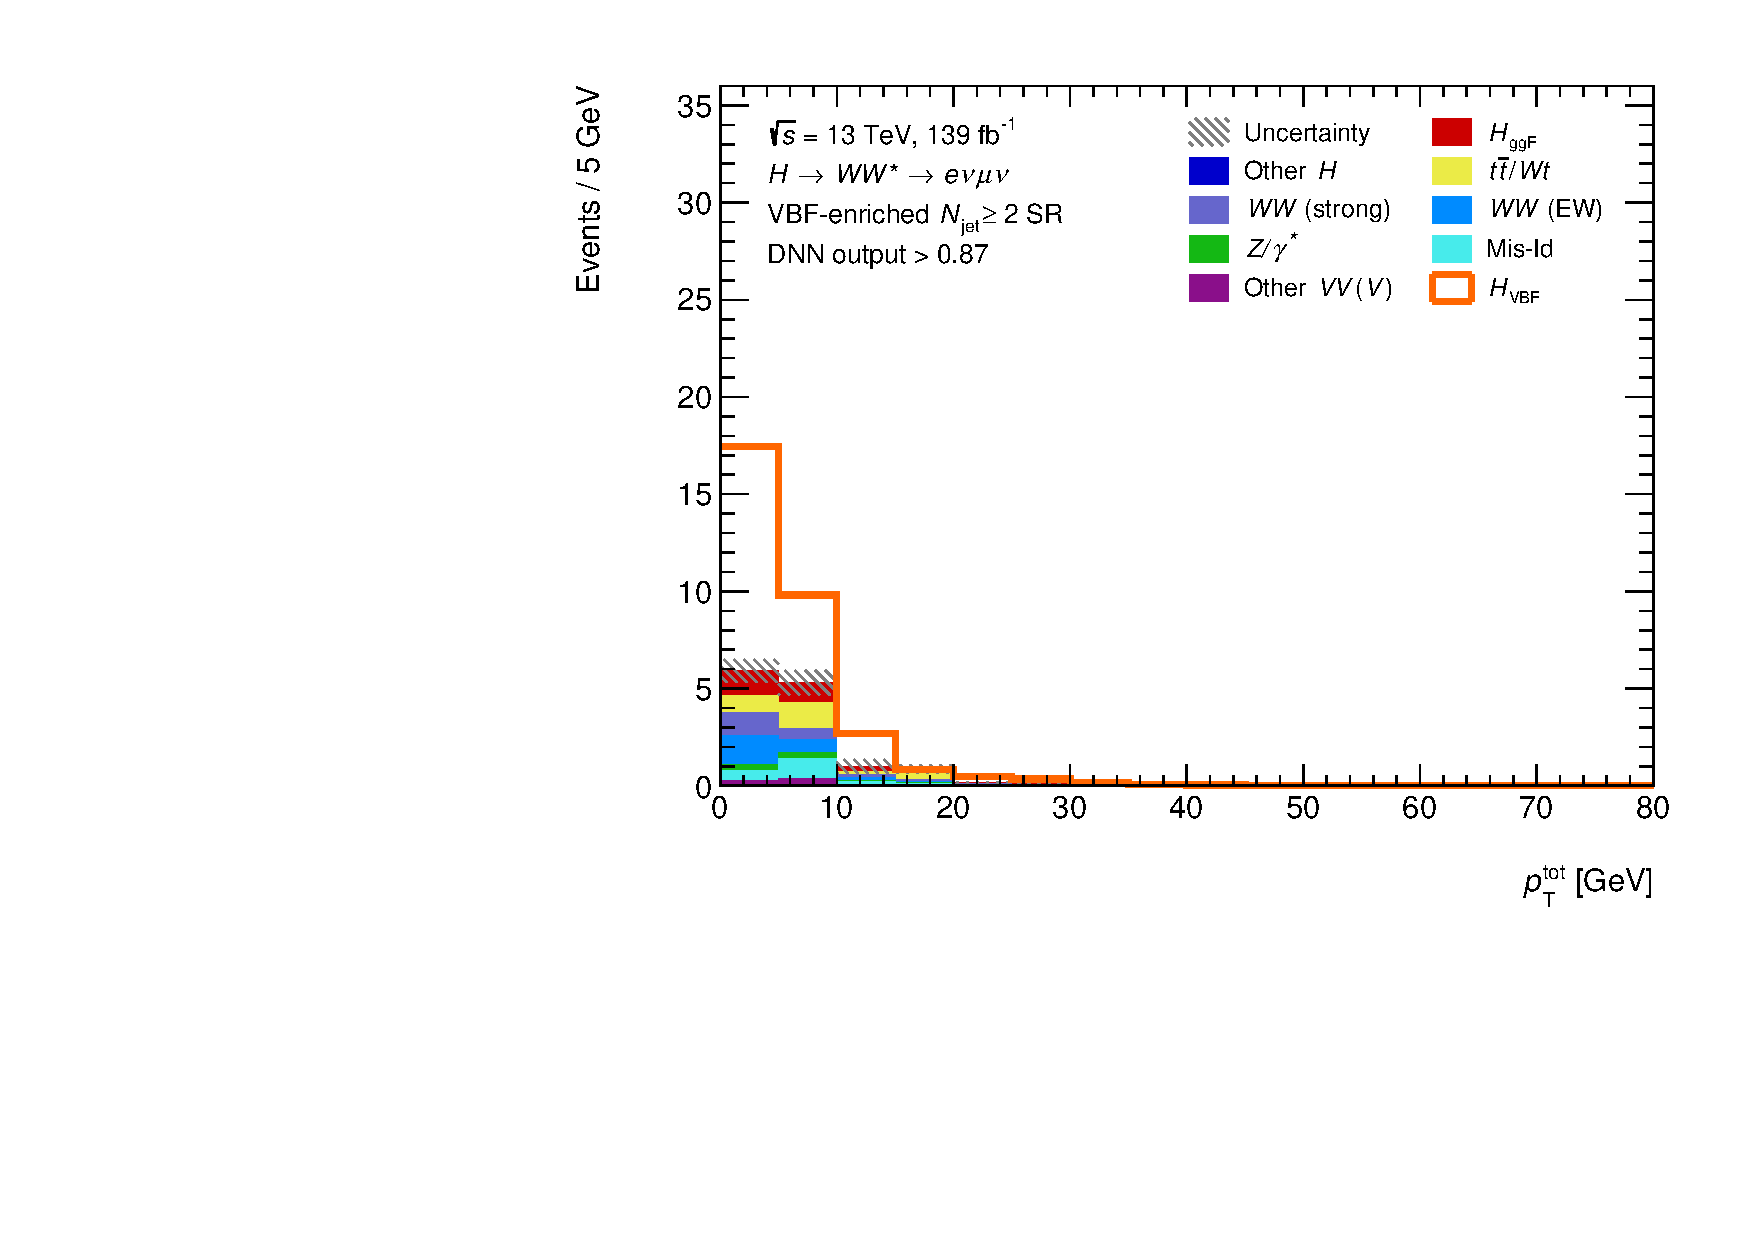
\includegraphics[width=0.32\textwidth]{figures/hww/dnn/blinded/run2-emme-CutVBFSR_DNN87-PtTot-lin.pdf}
        } \\
        \subfloat[$\METSig$]{
            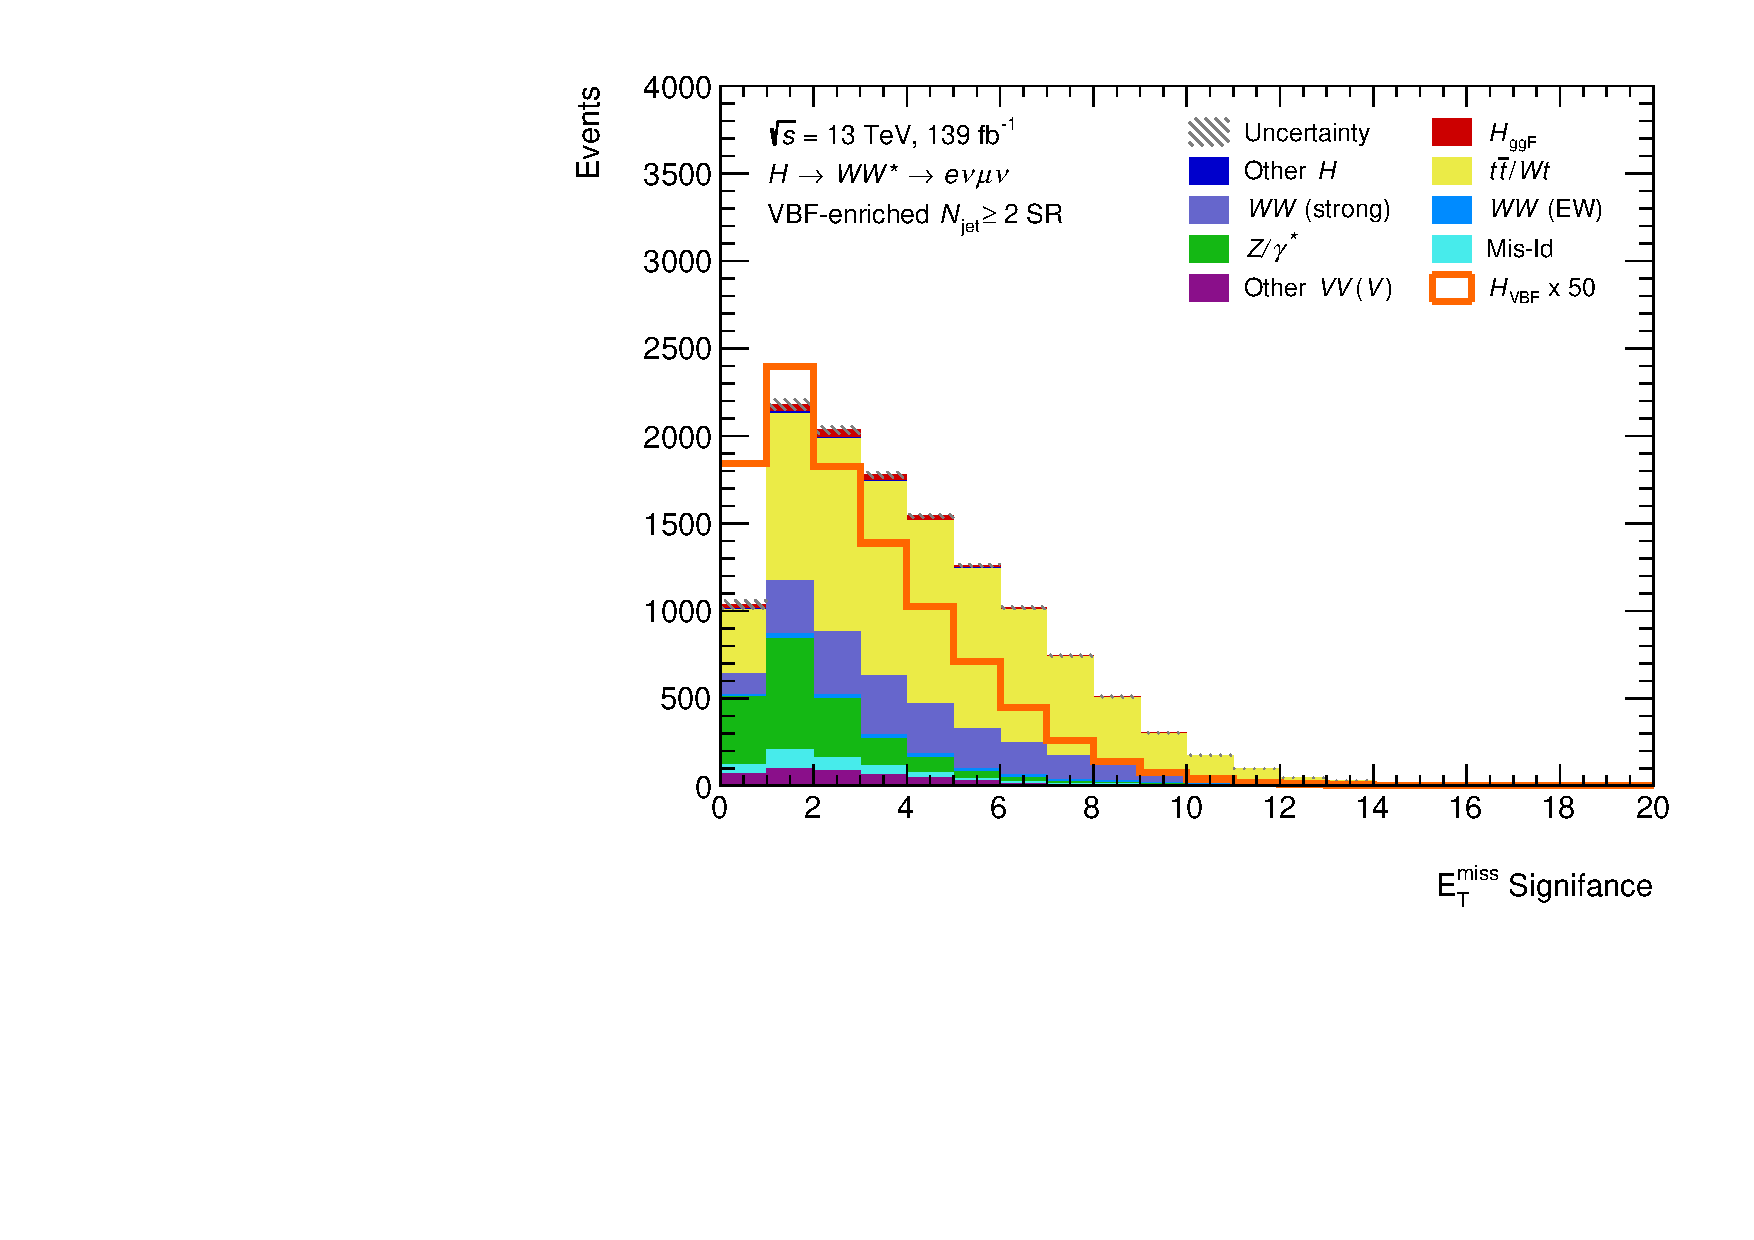
\includegraphics[width=0.32\textwidth]{figures/hww/dnn/blinded/run2-emme-CutVBF_SR-METSig_broad-lin.pdf} \hfill
            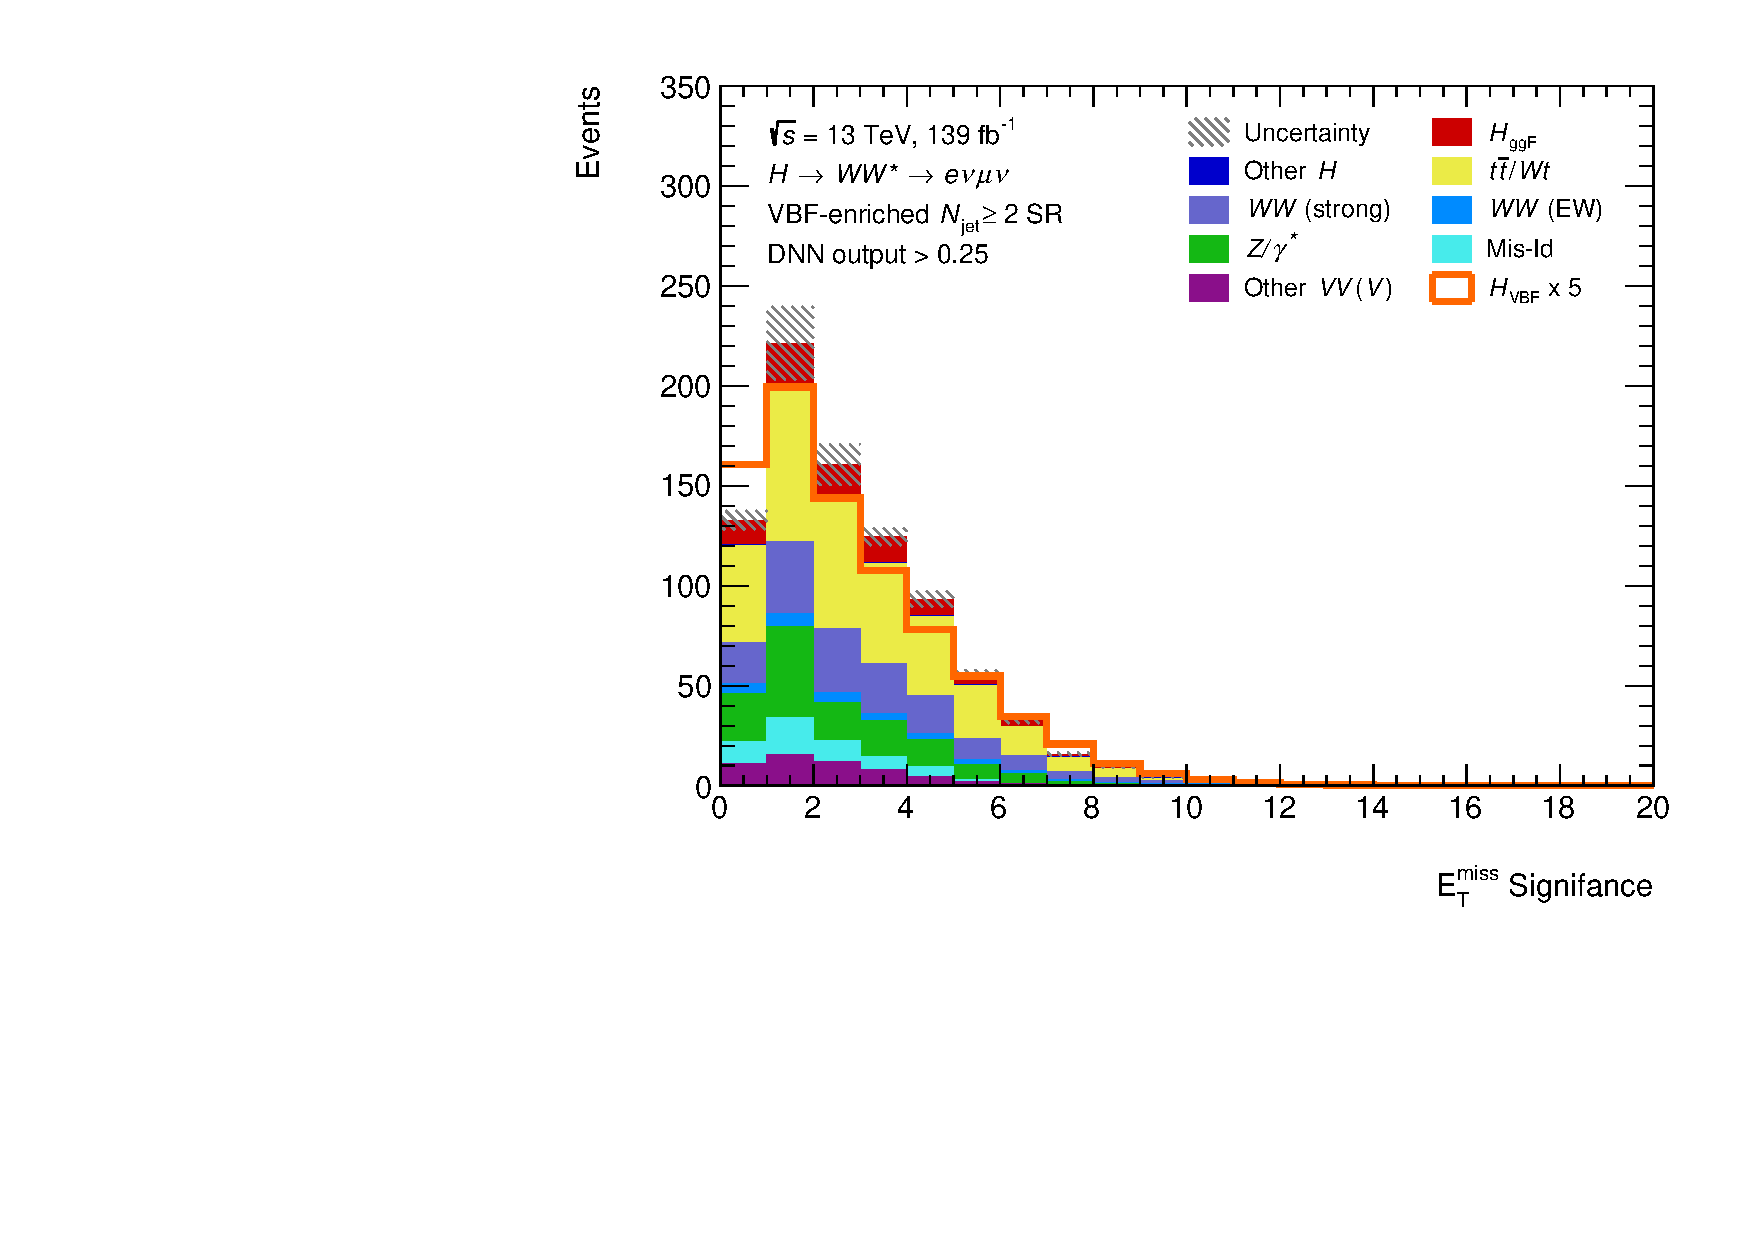
\includegraphics[width=0.32\textwidth]{figures/hww/dnn/blinded/run2-emme-CutVBFSR_DNN25-METSig_broad-lin.pdf} \hfill
            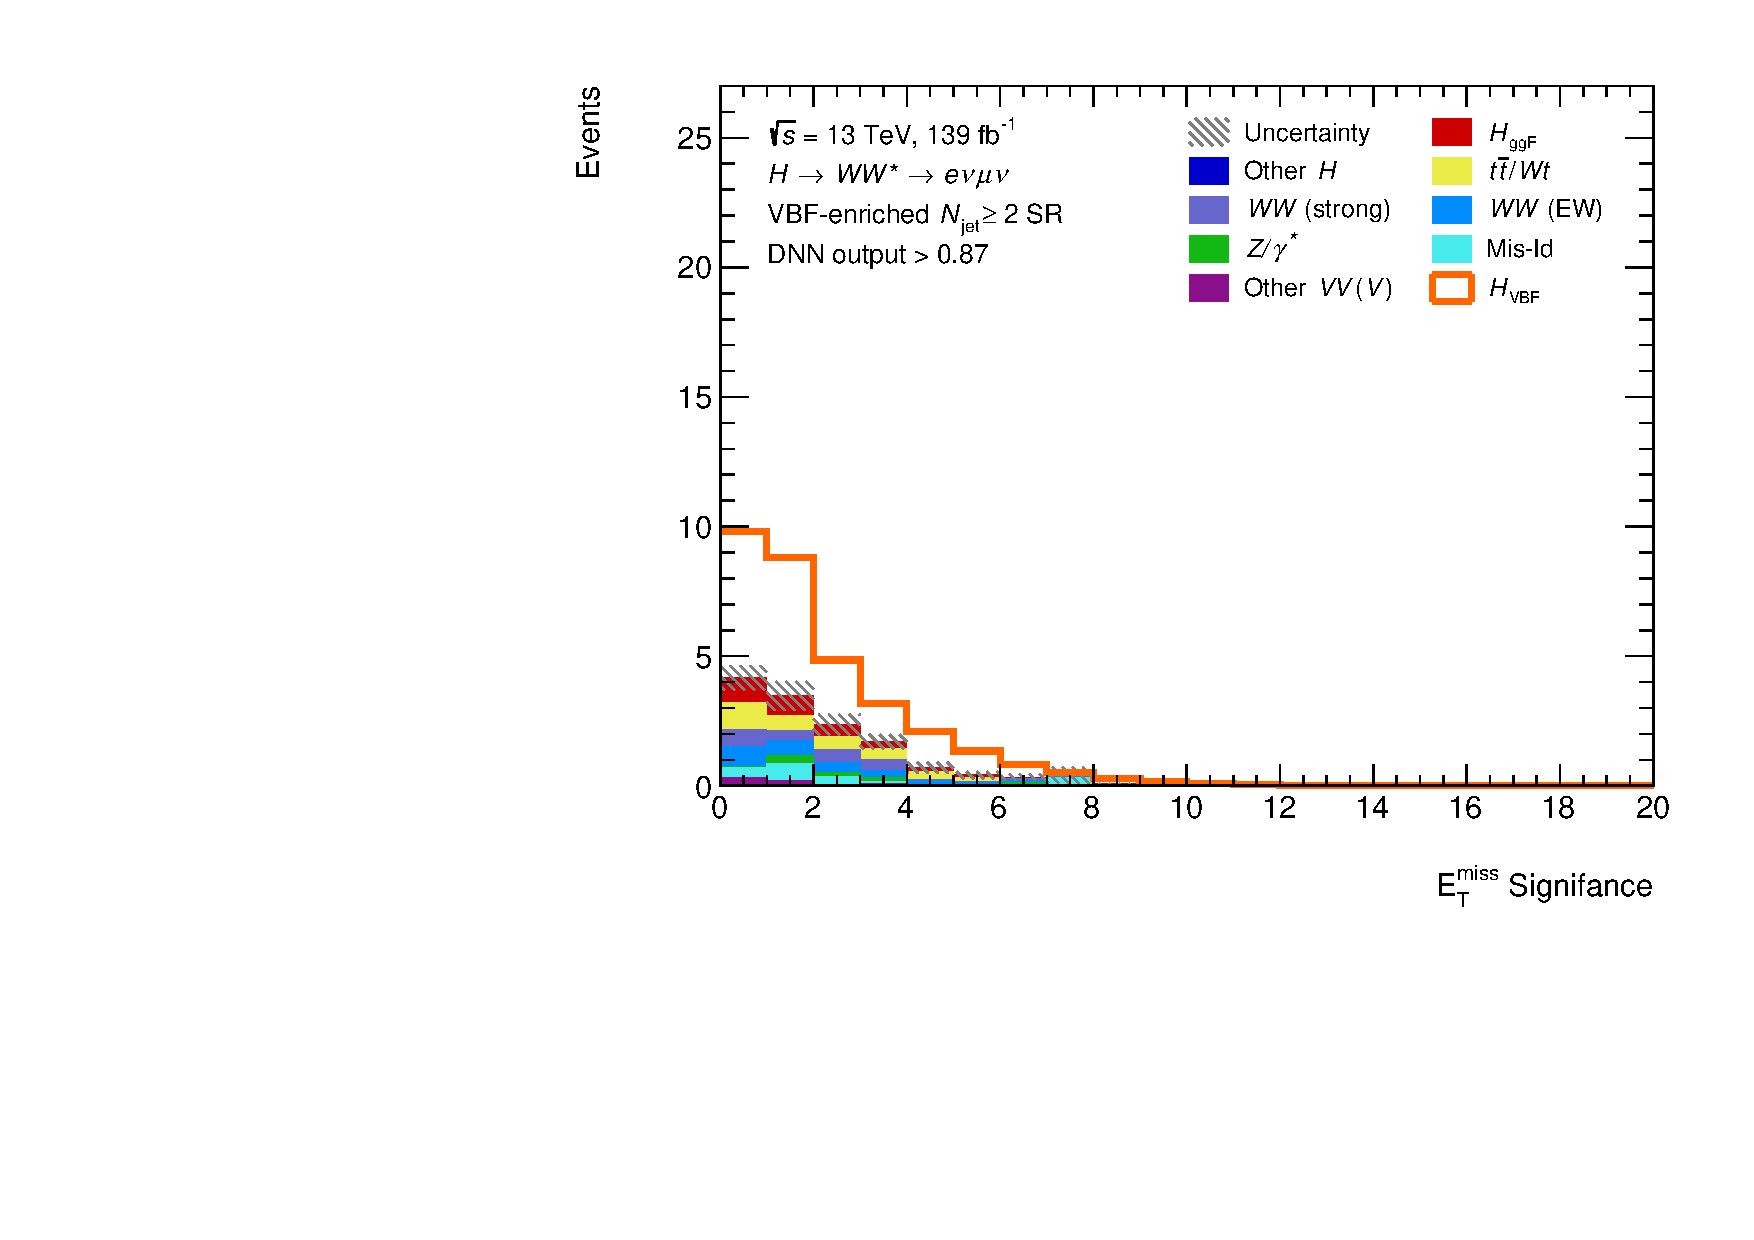
\includegraphics[width=0.32\textwidth]{figures/hww/dnn/blinded/run2-emme-CutVBFSR_DNN87-METSig_broad-lin.pdf}
        } \\
        {\caption[Distributions of $\pttot$ and $\METSig$ in the VBF \TwoJet signal region.]{Distributions of $\pttot$ and $\METSig$ in the VBF \TwoJet signal region.
            Each row corresponds to one variable with different selections made on the DNN output as indicated in the figure. The solid orange line shows the expected VBF signal scaled by a factor of (left) 50, (center) 5, and (right) without any scaling.
            \label{app:fig:dnn-inputs-top-sup} }}
    \end{figure}

    \FloatBarrier
    \section{DNN output distributions in the VBF STXS CRs}
    \Cref{app:fig:dnn-output-vbf-stxs} shows the distributions of the DNN output in the top-quark and \Ztautau CRs used in the VBF, STXS analysis prior to the statistical analyiss.
    The distributions confirm that the data are modelled well by the MC simulation.

    \begin{figure}[h!]
        \centering
        \subfloat[{\tiny $350 \leq \mjj < 700~\GeV, \pTH < 200~\GeV$}]{
            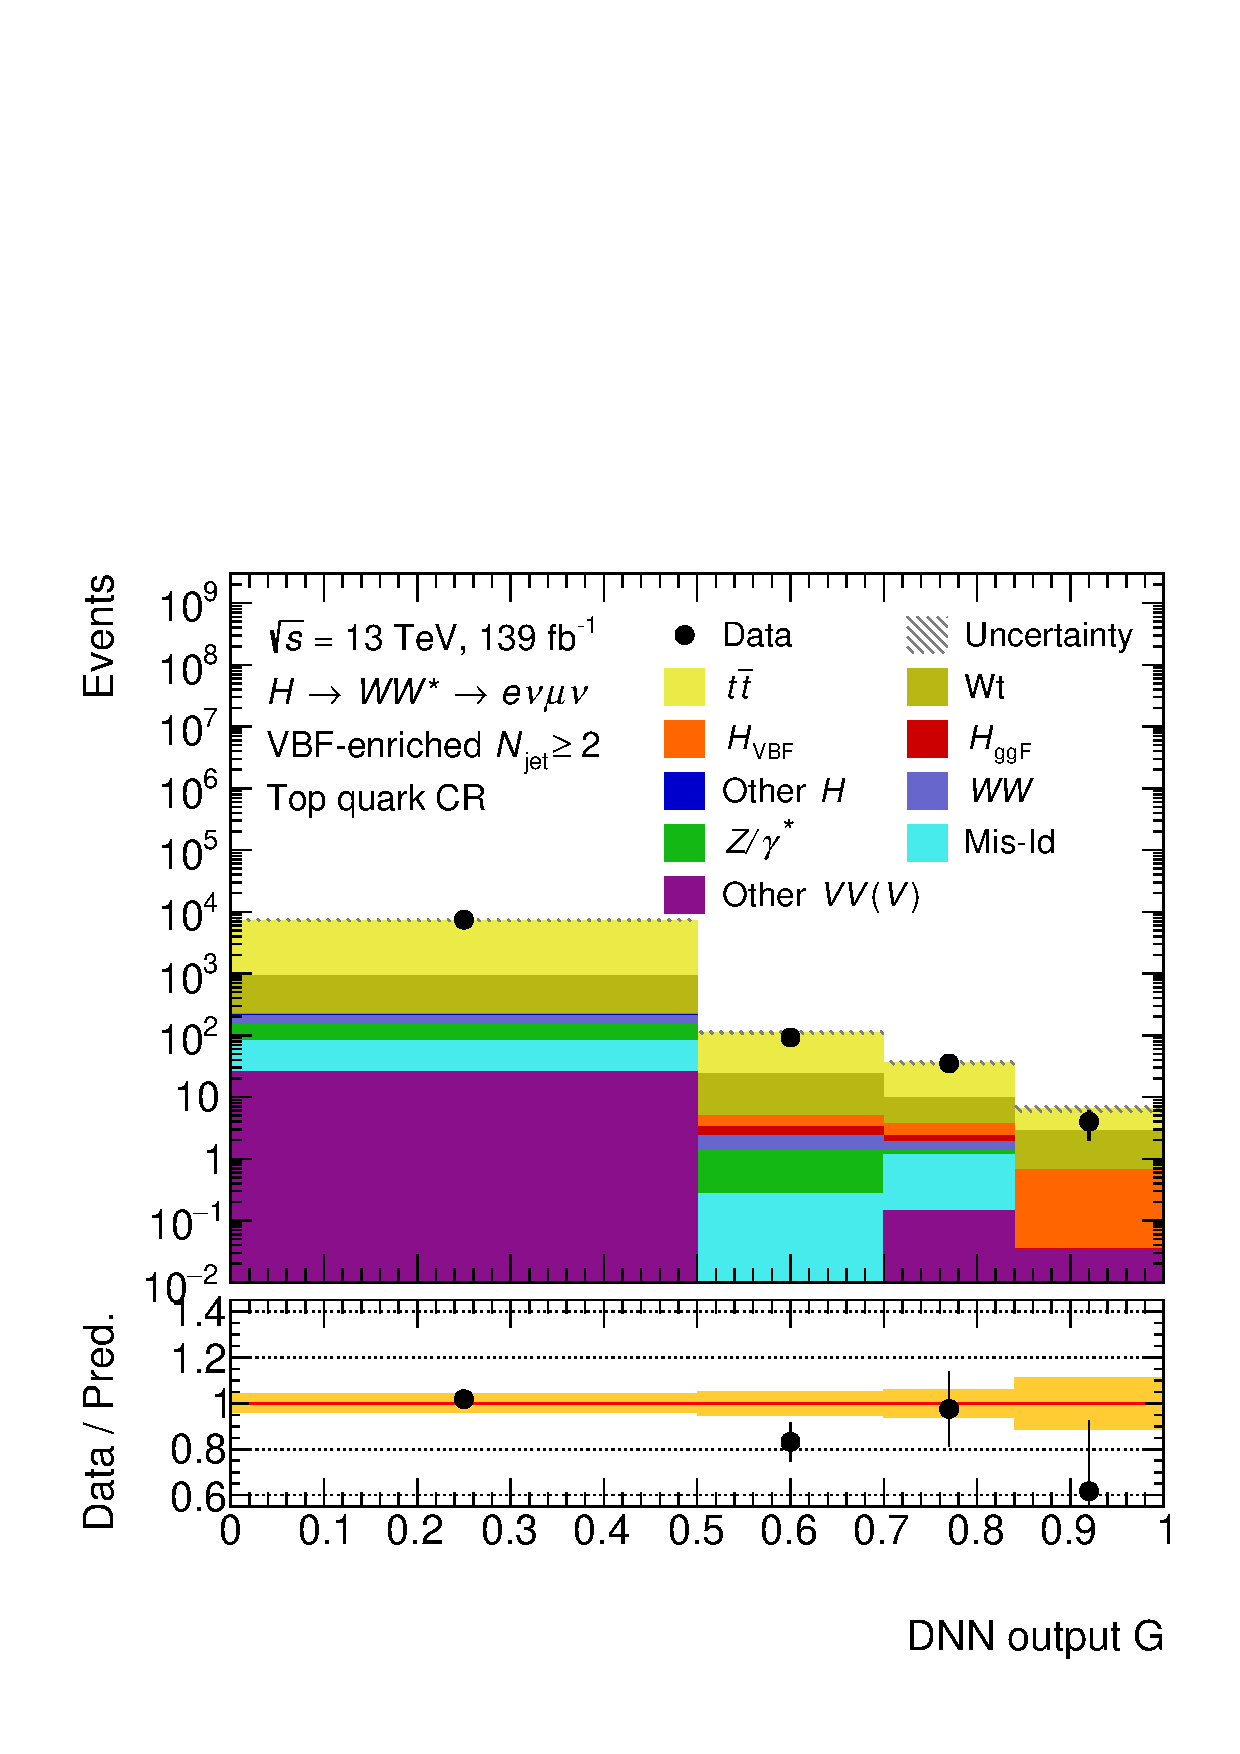
\includegraphics[width=0.32\textwidth]{figures/220605-Thesis/topcr/stxs/plots/run2-emme-CutVBF_TopControl_2jet_MJJ_350_700_PTH_0_200-DNNoutputG_FitBin1-log.pdf} \hfill
        }
        \subfloat[{\tiny $\mjj \geq 700~\GeV, \pTH < 200~\GeV$}]{
            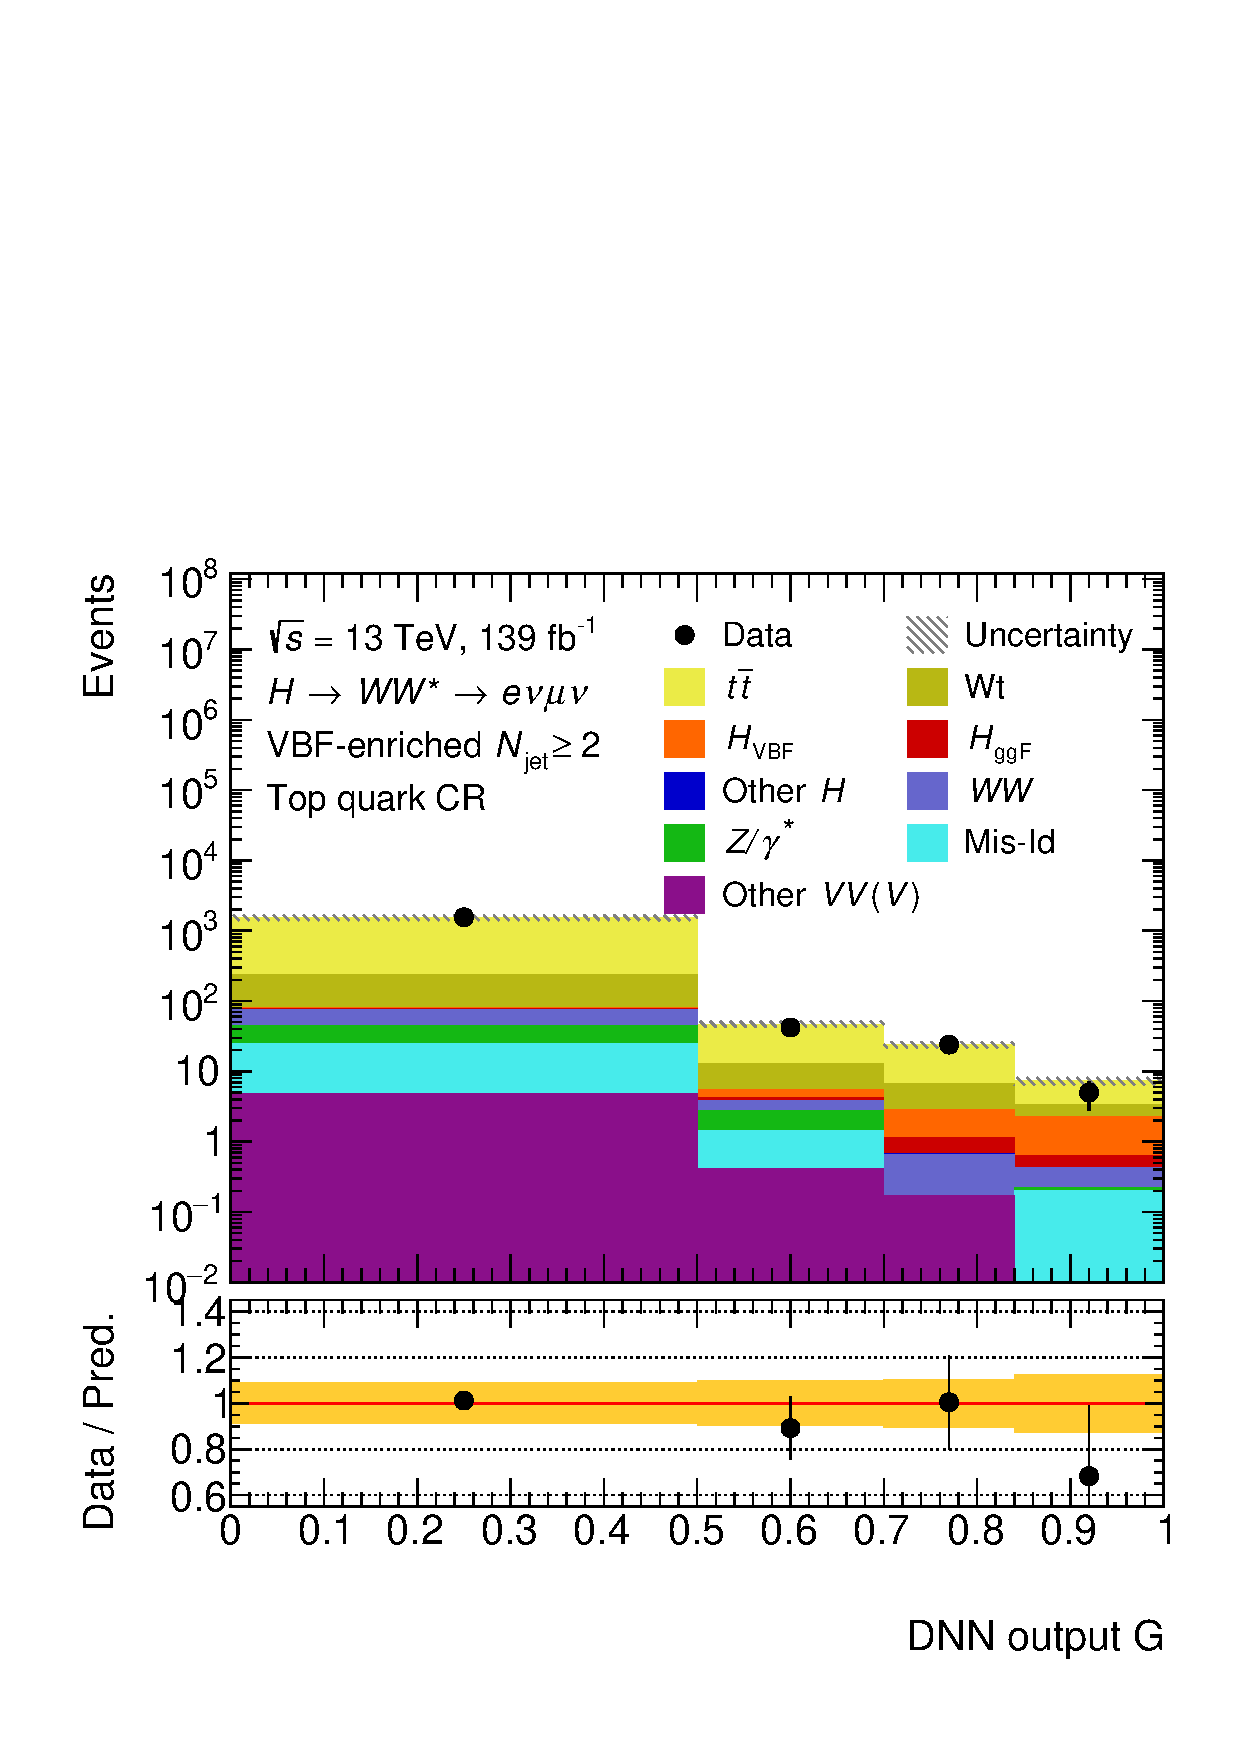
\includegraphics[width=0.32\textwidth]{figures/220605-Thesis/topcr/stxs/plots/run2-emme-CutVBF_TopControl_2jet_MJJ_GT700_PTH_0_200-DNNoutputG_FitBin1-log.pdf} \hfill
        }
        \subfloat[{\tiny $\mjj \geq 350~\GeV, \pTH \geq 200~\GeV$}]{
            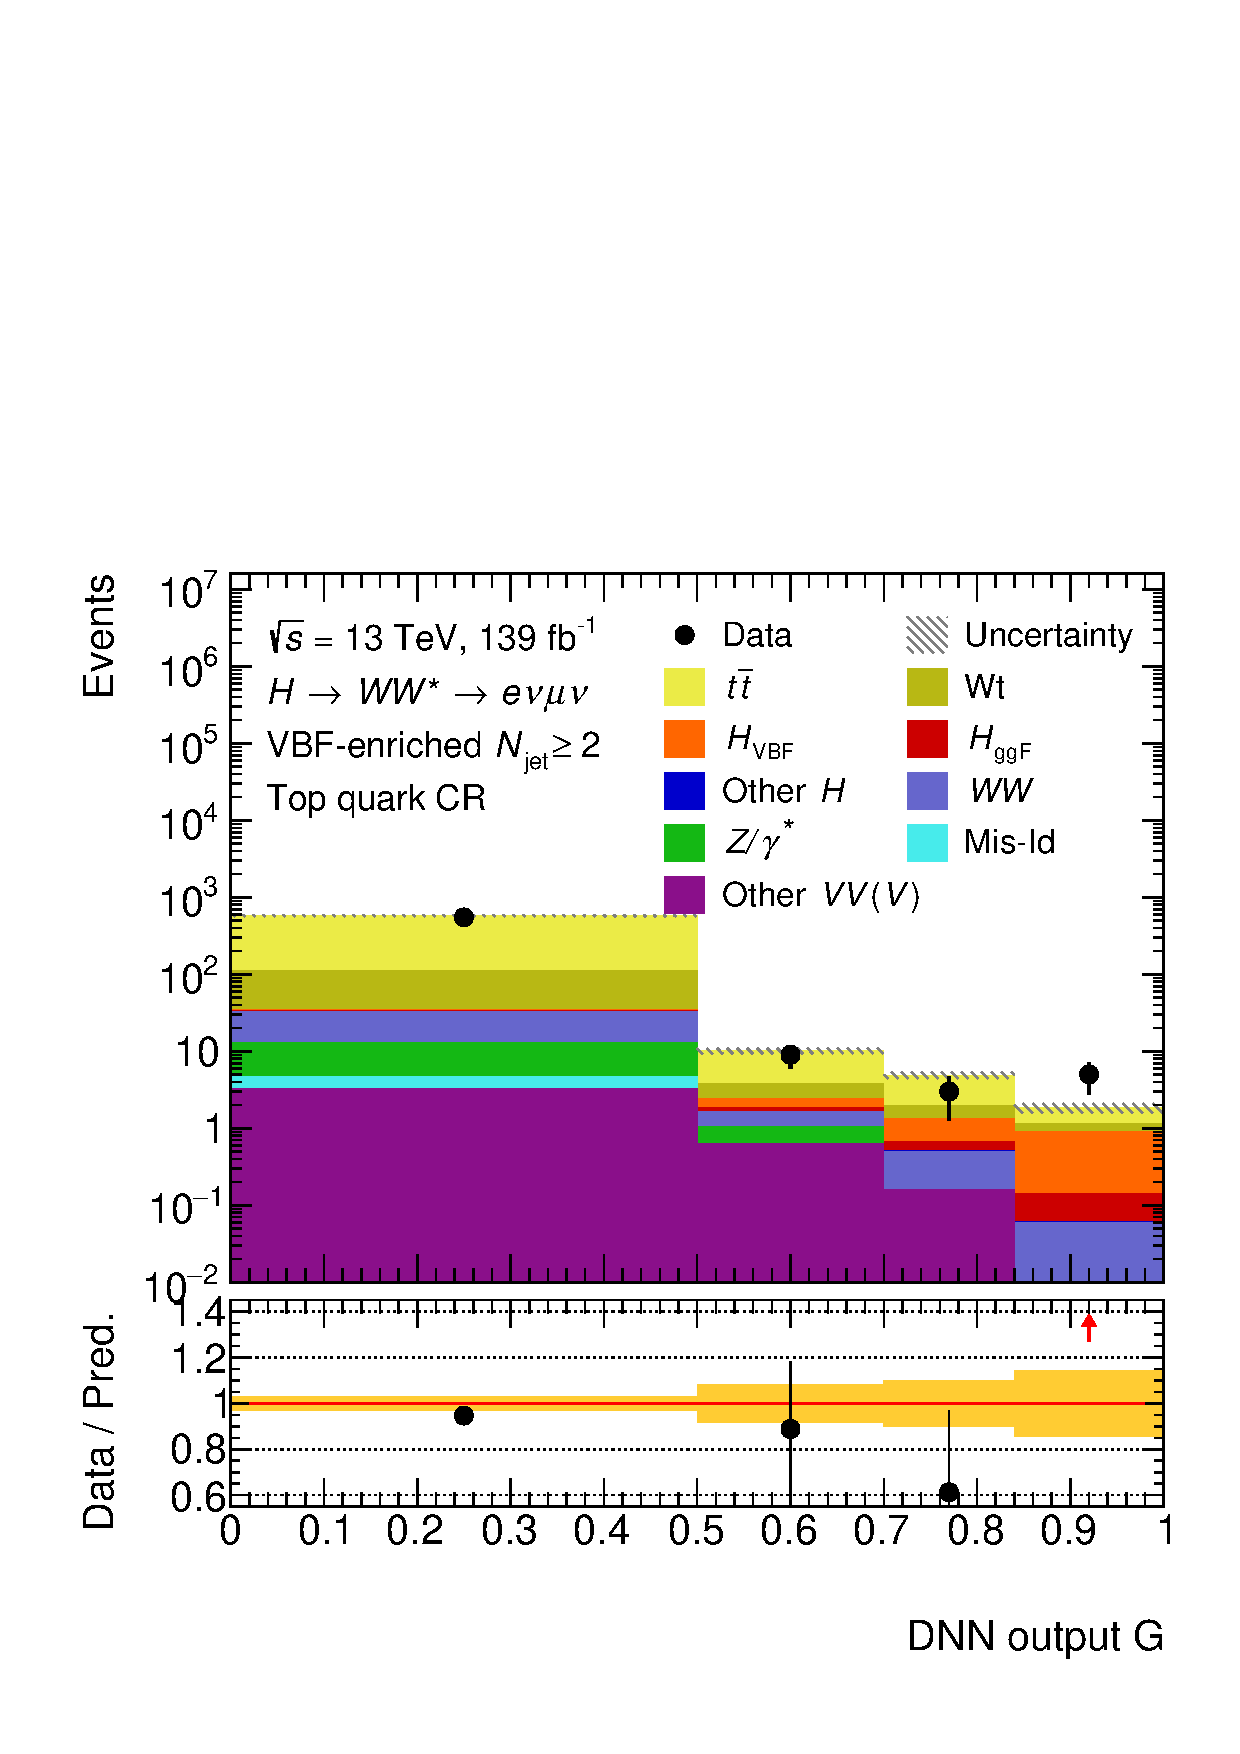
\includegraphics[width=0.32\textwidth]{figures/220605-Thesis/topcr/stxs/plots/run2-emme-CutVBF_TopControl_2jet_MJJ_GT350_PTH_GT200-DNNoutputG_FitBin1-log.pdf} \hfill
        }  \\
        \subfloat[{\tiny $350 \leq \mjj < 700~\GeV, \pTH < 200~\GeV$}]{
            \includegraphics[width=0.32\textwidth]{figures/220605-Thesis/zttcr/stxs/plots/run2-emme-CutVBF_ZtautauControl_2jet_MJJ_350_700_PTH_0_200-DNNoutputG_FitBin1-log.pdf} \hfill
        }
        \subfloat[{\tiny $\mjj \geq 700~\GeV, \pTH < 200~\GeV$}]{
            \includegraphics[width=0.32\textwidth]{figures/220605-Thesis/zttcr/stxs/plots/run2-emme-CutVBF_ZtautauControl_2jet_MJJ_GT700_PTH_0_200-DNNoutputG_FitBin1-log.pdf} \hfill
        }
        \subfloat[{\tiny $\mjj \geq 350~\GeV, \pTH \geq 200~\GeV$}]{
            \includegraphics[width=0.32\textwidth]{figures/220605-Thesis/zttcr/stxs/plots/run2-emme-CutVBF_ZtautauControl_2jet_MJJ_GT350_PTH_GT200-DNNoutputG_FitBin1-log.pdf} \hfill
        }
        \caption[Distributions of the DNN output in the control regions used in the VBF STXS analysis.]{
            Distributions of the DNN output in (a)-(c) the top-quark control regions and (d)-(f) the \Ztautau control regions used in the VBF STXS analysis with the selections indicated for each subfigure. The yellow band corresponds to the square root of the sum in quadrature of the MC statistical uncertainties and the normalization component of the dominant experimental systematic uncertainties (JER, JES, Flavor-tagging, and \MET uncertainties). The various uncertainty components are discussed in more detail in \cref{sec:systematics}.}
        \label{app:fig:dnn-output-vbf-stxs}
    \end{figure}

    \FloatBarrier
    \section{Expected number of events at different selection stages}
    \label{app:cutflows}

    \Cref{app:tab:cutflows} shows the expected number of events at different selection stages to define the VBF \TwoJet SRs and CRs and the ggF \TwoJet SRs and CRS.

    \begin{landscape}
        \thispagestyle{empty}
        \begin{table}
            \subfloat[]{
                \resizebox{\textwidth}{!}{
                    %%% created on Wed Jun 15 01:04:43 2022 from TQSampleFolder 'samples' with TQLibrary UNKNOWN compiled with GCC 8.3.0 against ROOT 6.18/04
\providecommand{\xmark}{{\sffamily \bfseries X}}
\providecommand\rotatecell[2]{\rotatebox[origin=c]{#1}{#2}}
\begin{tabular}{ r || r  r  r | r  r  r  r  r  r | r  r }
\ensuremath{\sqrt{s}=13\,}TeV, 139 fb$^{-1}$ & $H_{VBF}$ & $H_{ggF}$ & Other $H$ & Top & $WW$ (Strong) & $WW$ (EW) & $Z/\gamma^{*}$ & Mis-Id & Other $VV$($V$) & Total Bkg & Data\tabularnewline
\hline
Preselection & \ensuremath{597.44\pm 0.74} & \ensuremath{5626.30\pm 7.79} & \ensuremath{2098.36\pm 2.72} & \ensuremath{1158767.99\pm 236.35} & \ensuremath{126397.14\pm 115.16} & \ensuremath{1067.67\pm 2.02} & \ensuremath{255778.21\pm 429.05} & \ensuremath{32969.04\pm 243.45} & \ensuremath{20099.62\pm 103.68} & \ensuremath{1600705.98\pm 568.59} & \ensuremath{1585575}\tabularnewline
\hline
\TwoJet & \ensuremath{366.95\pm 0.58} & \ensuremath{1061.65\pm 3.08} & \ensuremath{769.79\pm 1.39} & \ensuremath{916426.43\pm 203.00} & \ensuremath{24253.86\pm 30.33} & \ensuremath{879.26\pm 1.83} & \ensuremath{26050.68\pm 106.57} & \ensuremath{11627.40\pm 161.67} & \ensuremath{5216.69\pm 49.46} & \ensuremath{985515.98\pm 286.50} & \ensuremath{975285}\tabularnewline
$\Nbjetsub=0$ & \ensuremath{324.06\pm 0.54} & \ensuremath{914.40\pm 2.86} & \ensuremath{445.15\pm 1.16} & \ensuremath{64086.49\pm 57.56} & \ensuremath{20989.02\pm 28.72} & \ensuremath{761.52\pm 1.69} & \ensuremath{21857.05\pm 100.95} & \ensuremath{3836.65\pm 68.22} & \ensuremath{4115.48\pm 45.38} & \ensuremath{116560.61\pm 145.10} & \ensuremath{109428}\tabularnewline
$\mtt\,{<}\,m_Z - 25~\GeV$ & \ensuremath{278.43\pm 0.50} & \ensuremath{798.62\pm 2.68} & \ensuremath{198.24\pm 0.76} & \ensuremath{39059.60\pm 44.87} & \ensuremath{12209.30\pm 22.70} & \ensuremath{391.10\pm 1.21} & \ensuremath{7756.85\pm 70.31} & \ensuremath{2378.72\pm 51.42} & \ensuremath{2206.51\pm 36.12} & \ensuremath{64800.70\pm 106.91} & \ensuremath{61311}\tabularnewline
$\mjj > 120\ \GeV$ & \ensuremath{254.30\pm 0.48} & \ensuremath{488.43\pm 2.07} & \ensuremath{97.17\pm 0.53} & \ensuremath{26982.66\pm 36.93} & \ensuremath{8209.18\pm 17.75} & \ensuremath{335.95\pm 1.12} & \ensuremath{5105.96\pm 56.93} & \ensuremath{1386.09\pm 40.53} & \ensuremath{1494.00\pm 26.94} & \ensuremath{44002.26\pm 85.41} & \ensuremath{41466}\tabularnewline
CJV & \ensuremath{235.21\pm 0.46} & \ensuremath{416.07\pm 1.92} & \ensuremath{76.90\pm 0.48} & \ensuremath{21266.00\pm 33.12} & \ensuremath{6822.28\pm 16.77} & \ensuremath{291.77\pm 1.05} & \ensuremath{4334.52\pm 54.34} & \ensuremath{1092.99\pm 36.55} & \ensuremath{1221.76\pm 24.36} & \ensuremath{35445.39\pm 79.15} & \ensuremath{33802}\tabularnewline
OLV & \ensuremath{203.70\pm 0.43} & \ensuremath{201.86\pm 1.36} & \ensuremath{31.60\pm 0.31} & \ensuremath{7697.63\pm 20.03} & \ensuremath{2186.05\pm 10.73} & \ensuremath{196.98\pm 0.86} & \ensuremath{1686.28\pm 42.33} & \ensuremath{355.21\pm 21.82} & \ensuremath{437.44\pm 14.94} & \ensuremath{12761.45\pm 54.87} & \ensuremath{12189}\tabularnewline
\hline
VBF SR, DNN output $\leq 0.25$ & \ensuremath{38.94\pm 0.19} & \ensuremath{120.57\pm 1.05} & \ensuremath{27.93\pm 0.29} & \ensuremath{7361.63\pm 19.54} & \ensuremath{2026.09\pm 10.26} & \ensuremath{168.46\pm 0.80} & \ensuremath{1548.30\pm 37.24} & \ensuremath{303.00\pm 20.79} & \ensuremath{381.25\pm 13.71} & \ensuremath{11909.30\pm 49.96} & \ensuremath{11281}\tabularnewline
VBF SR, DNN output $> 0.25$ & \ensuremath{164.76\pm 0.39} & \ensuremath{81.29\pm 0.86} & \ensuremath{3.67\pm 0.10} & \ensuremath{336.00\pm 4.39} & \ensuremath{159.96\pm 3.14} & \ensuremath{28.52\pm 0.33} & \ensuremath{137.98\pm 20.13} & \ensuremath{52.21\pm 6.62} & \ensuremath{56.19\pm 5.94} & \ensuremath{852.14\pm 22.68} & \ensuremath{908}\tabularnewline
VBF SR, DNN output $> 0.87$ & \ensuremath{31.97\pm 0.17} & \ensuremath{2.81\pm 0.16} & \ensuremath{0.04\pm 0.01} & \ensuremath{3.06\pm 0.47} & \ensuremath{2.12\pm 0.29} & \ensuremath{2.50\pm 0.10} & \ensuremath{0.72\pm 0.27} & \ensuremath{1.81\pm 0.72} & \ensuremath{0.68\pm 0.15} & \ensuremath{13.71\pm 0.98} & \ensuremath{38}\tabularnewline
\hline
\hline
VBF \Zgamma CR & \ensuremath{17.29\pm 0.13} & \ensuremath{14.78\pm 0.36} & \ensuremath{19.30\pm 0.21} & \ensuremath{277.83\pm 3.77} & \ensuremath{82.53\pm 1.80} & \ensuremath{6.40\pm 0.15} & \ensuremath{1678.23\pm 17.93} & \ensuremath{11.62\pm 8.88} & \ensuremath{79.65\pm 6.42} & \ensuremath{2151.04\pm 21.43} & \ensuremath{2114}\tabularnewline
\hline
\hline
VBF Top CR & \ensuremath{22.49\pm 0.15} & \ensuremath{28.48\pm 0.52} & \ensuremath{10.95\pm 0.16} & \ensuremath{40218.20\pm 44.11} & \ensuremath{270.73\pm 3.47} & \ensuremath{20.50\pm 0.29} & \ensuremath{264.39\pm 10.19} & \ensuremath{404.69\pm 33.38} & \ensuremath{89.68\pm 6.86} & \ensuremath{41296.67\pm 56.77} & \ensuremath{41112}\tabularnewline
\hline
\hline
VBF $WW$ VR & \ensuremath{16.86\pm 0.12} & \ensuremath{42.90\pm 0.62} & \ensuremath{17.88\pm 0.23} & \ensuremath{8499.91\pm 21.78} & \ensuremath{5347.94\pm 13.44} & \ensuremath{339.27\pm 1.13} & \ensuremath{247.23\pm 13.36} & \ensuremath{429.50\pm 21.39} & \ensuremath{621.07\pm 12.85} & \ensuremath{15527.81\pm 38.18} & \ensuremath{14452}
\end{tabular}

                }
            } \\
            \vspace{20pt}
            \subfloat[]{
                \resizebox{\textwidth}{!}{
                    %%% created on Sat Jun 25 06:27:49 2022 from TQSampleFolder 'samples' with TQLibrary UNKNOWN compiled with GCC 8.3.0 against ROOT 6.18/04
\providecommand{\xmark}{{\sffamily \bfseries X}}
\providecommand\rotatecell[2]{\rotatebox[origin=c]{#1}{#2}}
\begin{tabular}{ r || r  r  r | r  r  r  r  r  r | r  r }
\ensuremath{\sqrt{s}=13\,}TeV, 139 fb$^{-1}$ & $H_{VBF}$ & $H_{ggF}$ & Other $H$ & Top & $WW$ (Strong) & $WW$ (EW) & $Z/\gamma^{*}$ & Mis-Id & Other $VV$($V$) & Total Bkg & Data\tabularnewline
\hline
%Preselection & \ensuremath{597.44\pm 0.74} & \ensuremath{5626.25\pm 7.79} & \ensuremath{2715.74\pm 2.81} & \ensuremath{1158769.79\pm 236.35} & \ensuremath{126397.19\pm 115.16} & \ensuremath{1067.67\pm 2.02} & \ensuremath{255779.21\pm 429.12} & \ensuremath{32980.49\pm 243.92} & \ensuremath{20030.20\pm 117.61} & \ensuremath{1600650.80\pm 571.54} & \ensuremath{1585575}\tabularnewline
Preselection & \ensuremath{597.44\pm 0.74} & \ensuremath{5626.30\pm 7.79} & \ensuremath{2098.36\pm 2.72} & \ensuremath{1158767.99\pm 236.35} & \ensuremath{126397.14\pm 115.16} & \ensuremath{1067.67\pm 2.02} & \ensuremath{255778.21\pm 429.05} & \ensuremath{32969.04\pm 243.45} & \ensuremath{20099.62\pm 103.68} & \ensuremath{1600705.98\pm 568.59} & \ensuremath{1585575}\tabularnewline
$p_{\textrm{T}}^{\textrm{miss}} > 20$\,GeV & \ensuremath{562.57\pm 0.72} & \ensuremath{5236.37\pm 7.52} & \ensuremath{1956.46\pm 2.18} & \ensuremath{1070098.87\pm 227.09} & \ensuremath{107828.31\pm 105.20} & \ensuremath{1004.45\pm 1.95} & \ensuremath{68604.79\pm 237.67} & \ensuremath{26836.67\pm 201.93} & \ensuremath{13941.13\pm 89.60} & \ensuremath{1293550.58\pm 409.86} & \ensuremath{1288321}\tabularnewline
\hline
$N_{\textrm{jet}} \geq 2$ & \ensuremath{346.39\pm 0.56} & \ensuremath{987.40\pm 2.97} & \ensuremath{1227.08\pm 1.42} & \ensuremath{847943.75\pm 195.32} & \ensuremath{22252.84\pm 28.63} & \ensuremath{832.46\pm 1.78} & \ensuremath{16484.46\pm 76.92} & \ensuremath{10509.47\pm 153.29} & \ensuremath{4455.03\pm 48.43} & \ensuremath{903465.41\pm 265.97} & \ensuremath{895198}\tabularnewline
$\Nbjetsub=0$ & \ensuremath{306.18\pm 0.53} & \ensuremath{850.54\pm 2.76} & \ensuremath{382.78\pm 1.03} & \ensuremath{59546.95\pm 55.50} & \ensuremath{19223.75\pm 27.09} & \ensuremath{721.18\pm 1.65} & \ensuremath{13641.23\pm 73.46} & \ensuremath{3419.84\pm 61.60} & \ensuremath{3502.85\pm 44.14} & \ensuremath{100906.34\pm 122.33} & \ensuremath{95323}\tabularnewline
$\mtt\,{<}\,m_Z - 25~\GeV$  & \ensuremath{266.51\pm 0.49} & \ensuremath{757.09\pm 2.61} & \ensuremath{187.37\pm 0.71} & \ensuremath{37486.00\pm 43.98} & \ensuremath{11579.69\pm 21.89} & \ensuremath{376.46\pm 1.19} & \ensuremath{4790.34\pm 51.82} & \ensuremath{2164.97\pm 48.23} & \ensuremath{1947.81\pm 35.93} & \ensuremath{59102.36\pm 93.40} & \ensuremath{56165}\tabularnewline
$\mll<55$\,GeV & \ensuremath{238.10\pm 0.47} & \ensuremath{669.54\pm 2.45} & \ensuremath{111.78\pm 0.55} & \ensuremath{9861.44\pm 22.44} & \ensuremath{3075.76\pm 11.07} & \ensuremath{84.55\pm 0.56} & \ensuremath{2363.11\pm 34.08} & \ensuremath{875.70\pm 28.47} & \ensuremath{850.30\pm 28.66} & \ensuremath{17780.40\pm 58.53} & \ensuremath{17165}\tabularnewline
$\DPhill < 1.8$ & \ensuremath{231.34\pm 0.46} & \ensuremath{643.72\pm 2.40} & \ensuremath{104.00\pm 0.53} & \ensuremath{9364.87\pm 21.90} & \ensuremath{2889.93\pm 10.65} & \ensuremath{80.13\pm 0.55} & \ensuremath{1421.99\pm 27.98} & \ensuremath{774.91\pm 26.74} & \ensuremath{768.72\pm 27.33} & \ensuremath{15944.26\pm 53.33} & \ensuremath{15506}\tabularnewline
$\Delta \dyjj > 1.2 || |m_{jj}-85| > 15$\,GeV & \ensuremath{226.58\pm 0.46} & \ensuremath{584.26\pm 2.28} & \ensuremath{72.90\pm 0.44} & \ensuremath{8460.40\pm 20.81} & \ensuremath{2636.53\pm 10.24} & \ensuremath{74.35\pm 0.53} & \ensuremath{1318.53\pm 27.31} & \ensuremath{659.31\pm 25.31} & \ensuremath{701.16\pm 26.87} & \ensuremath{14434.54\pm 51.49} & \ensuremath{14010}\tabularnewline
fail OLV $||$ fail CJV & \ensuremath{55.54\pm 0.22} & \ensuremath{405.20\pm 1.89} & \ensuremath{56.40\pm 0.38} & \ensuremath{6033.24\pm 17.50} & \ensuremath{1973.15\pm 8.63} & \ensuremath{29.23\pm 0.33} & \ensuremath{1036.03\pm 17.27} & \ensuremath{513.30\pm 22.14} & \ensuremath{503.02\pm 23.84} & \ensuremath{10493.16\pm 41.72} & \ensuremath{9982}\tabularnewline
\hline
ggF $N_{\textrm{jet}} \geq 2$ SR, $10 < m_{\ell\ell}<30$\,GeV & \ensuremath{24.84\pm 0.15} & \ensuremath{183.83\pm 1.27} & \ensuremath{23.16\pm 0.25} & \ensuremath{1825.09\pm 9.58} & \ensuremath{594.59\pm 4.56} & \ensuremath{9.26\pm 0.19} & \ensuremath{267.36\pm 14.78} & \ensuremath{181.86\pm 14.75} & \ensuremath{228.29\pm 19.35} & \ensuremath{3290.28\pm 30.41} & \ensuremath{3163}\tabularnewline
ggF $N_{\textrm{jet}} \geq 2$ SR,	$30 < m_{\ell\ell}<55$\,GeV & \ensuremath{30.71\pm 0.17} & \ensuremath{221.37\pm 1.40} & \ensuremath{33.24\pm 0.30} & \ensuremath{4208.14\pm 14.64} & \ensuremath{1378.55\pm 7.32} & \ensuremath{19.98\pm 0.27} & \ensuremath{768.67\pm 8.93} & \ensuremath{331.45\pm 16.50} & \ensuremath{274.73\pm 13.92} & \ensuremath{7202.88\pm 28.56} & \ensuremath{6819}\tabularnewline
\hline
\hline
ggF \TwoJet top-quark CR & \ensuremath{0.06\pm 0.01} & \ensuremath{0.49\pm 0.07} & \ensuremath{5.20\pm 0.11} & \ensuremath{4972.30\pm 15.96} & \ensuremath{1386.43\pm 6.91} & \ensuremath{33.65\pm 0.36} & \ensuremath{28.28\pm 3.09} & \ensuremath{183.77\pm 15.74} & \ensuremath{165.07\pm 6.99} & \ensuremath{6769.99\pm 24.67} & \ensuremath{6678}\tabularnewline
\hline
\hline
ggF \TwoJet $WW$ CR & \ensuremath{0.03\pm 0.00} & \ensuremath{0.13\pm 0.03} & \ensuremath{1.50\pm 0.06} & \ensuremath{563.92\pm 5.65} & \ensuremath{588.48\pm 4.50} & \ensuremath{22.10\pm 0.29} & \ensuremath{15.28\pm 2.06} & \ensuremath{27.92\pm 5.89} & \ensuremath{48.24\pm 3.17} & \ensuremath{1266.07\pm 10.06} & \ensuremath{1140}\tabularnewline
\hline
\hline
ggF \TwoJet \Zgamma CR & \ensuremath{4.90\pm 0.07} & \ensuremath{27.60\pm 0.47} & \ensuremath{28.11\pm 0.29} & \ensuremath{435.51\pm 4.54} & \ensuremath{186.22\pm 2.31} & \ensuremath{3.80\pm 0.12} & \ensuremath{3059.61\pm 22.78} & \ensuremath{34.10\pm 11.07} & \ensuremath{181.23\pm 10.95} & \ensuremath{3928.06\pm 28.07} & \ensuremath{3624}
\tabularnewline
\end{tabular}

                }
            }
            \caption[Expected number of events at different selection stages.]{Expected number of events at different selection stages to define the (a) VBF \TwoJet SRs and CRs and (b) the ggF \TwoJet SRs and CRs. For (a) the selections from the row labelled ``Preselection'' to the row labelled ``OLV'' are applied subsequently; for (b) the selections from the row labelled ``Preselection'' to the row labelled ``fail OLV $||$ fail CJV'' are applied subsequently. All respective other rows include all selections that define the indicated regions as described in \cref{sec:event-selection}.}
            \label{app:tab:cutflows}
        \end{table}
    \end{landscape}

    % \FloatBarrier
    % \section{Post-fit Distributions of the DNN input variables}
    % \label{app:post-fit-distributions}
    % \TDinote{}{MAYBE!?}
    % Not for now!


    \clearpage
    \FloatBarrier
    \section{Distributions in the ggF \ZeroJet and \OneJet Category}
    \label{app:event-selection-ggf}

    The distributions shown in \cref{app:fig:ggf:Plots:selections} illustrate the event selections made to define the ggF \ZeroJet and \OneJet category. This motivates the selections and reveals the background processes that are primarily suppressed by each requirement.

    \begin{figure}[!h]
        \centering
        \subfloat[]{
            \includegraphics[width=0.47\textwidth]{\paperfiguredir/ggF/ZeroJet/CutGGF_Ptll_0jet-Mll}
            \label{app:fig:ggf:Plots:selections-a}
        }
        \subfloat[]{
            \includegraphics[width=0.47\textwidth]{\paperfiguredir/ggF/ZeroJet/CutGGF_bVeto_0jet-DPhill}
            \label{app:fig:ggf:Plots:selections-b}
        } \\
        \subfloat[]{
            \includegraphics[width=0.47\textwidth]{\paperfiguredir/ggF/OneJet/CutGGF_ZttVeto_1jet-Mll}
            \label{app:fig:ggf:Plots:selections-c}
        }
        \subfloat[]{
            \includegraphics[width=0.47\textwidth]{\paperfiguredir/ggF/OneJet/CutGGF_TopoMll_1jet-DPhill}
            \label{app:fig:ggf:Plots:selections-d}
        }
        \caption[Distributions of \mll\ and \dphill\ in the \ZeroJet and \OneJet\ category.]{
            Distributions of (a) \mll\ and (b) \dphill\ in the \ZeroJet category as well as (c) \mll\ and (d) \dphill\ in the \OneJet category, after the preselection and background rejection steps, and also after the selection on \mll\ for the \dphill plots. The dashed lines indicate where the selection on the observable is made. The hatched band shows the normalization component of the total pre-fit uncertainty, assuming SM Higgs boson production. The bottom panels show the normalized distributions for the signal and backgrounds, from which it can be inferred which background processes are primarily removed by the indicated selections.
            Figure and caption taken from \ccite{HWWPaper}.
            \label{app:fig:ggf:Plots:selections}
        }
    \end{figure}

    \clearpage
    \FloatBarrier
    \section{Post-fit distributions in all CRs}
    \label{app:post-fit-cr-dists}

    \Cref{app:fig:Top_CRs,app:fig:Ztt_CRs,app:fig:WW_CRs} show the post-fit distributions of the CRs that enter the 2-PoI fit for the measurement of the inclusive VBF and ggF production cross section.
    Excellent agreement between the data and the SM predictions are observed.
    \begin{figure}[htp]
        \centering
        \subfloat[]{
            \includegraphics[width=0.47\textwidth]{\paperfiguredir/CRs/ggF0jet_WWCR_MT}
        }
        \subfloat[]{
            \includegraphics[width=0.47\textwidth]{\paperfiguredir/CRs/ggF1jet_WWCR_MT}
        } \\
        \subfloat[]{
            \includegraphics[width=0.47\textwidth]{\paperfiguredir/CRs/ggF2jet_WWCR_MT}
        }
        % \subfloat[]{
        %   \includegraphics[width=0.5\textwidth]{figures/VBF/CR/WW/DNNoutputG_Fit_finelowDNN2}
        % }
        \caption[Post-fit $\mT$ distributions in the ggF $WW$ control regions.]{
            Post-fit $\mT$ distributions in the (a) \ZeroJet, (b) \OneJet, and (c) ggF-enriched \TwoJet $WW$ CRs with signal (normalized to post-fit measurement) and background modeled contributions.
            The red arrow in the lower panel of (a) indicates that the central value of the data lies above the window. The last bin of each distribution is inclusive (includes the overflow).
            The hatched band shows the total uncertainty, assuming SM Higgs boson production.
            Some contributions are too small to be visible.
            Figure and caption taken from \ccite{HWWPaper}.
            \label{app:fig:WW_CRs}
        }
    \end{figure}
    \begin{figure}[htp]
        \centering
        \subfloat[]{
            \includegraphics[width=0.47\textwidth]{\paperfiguredir/CRs/ggF0jet_TopCR_MT}
        }
        \subfloat[]{
            \includegraphics[width=0.47\textwidth]{\paperfiguredir/CRs/ggF1jet_TopCR_MT}
        } \\
        \subfloat[]{
            \includegraphics[width=0.47\textwidth]{\paperfiguredir/CRs/ggF2jet_TopCR_MT}
        }
        \subfloat[]{
            \includegraphics[width=0.47\textwidth]{\paperfiguredir/VBF/CR/Top/DNNoutputG_Fit_finelowDNN2}
        }
        \caption[Post-fit \mT distributions in the ggF top-quark control regions.]{
            Post-fit \mT distributions in the (a) \ZeroJet, (b) \OneJet, and (c) ggF-enriched \TwoJet top quark CRs, as well as (d) the post-fit DNN output distribution in the VBF-enriched \TwoJet top quark CR, with signal (normalized to post-fit measurement) and background modeled contributions.
            The first two bins of the DNN output distribution used in the final fit, $[0$--$0.25,0.25$--$0.52]$, are here split into four bins, $[0$--$0.1,0.1$--$0.25,0.25$--$0.4,0.4$--$0.52]$, to illustrate the shape of the steeply falling background.
            The red arrows in the lower panel of (c) indicate that the central value of the data lies above the window. The last bin of each \mT distribution is inclusive (includes the overflow).
            The hatched band shows the total uncertainty, assuming SM Higgs boson production.
            Some contributions are too small to be visible.
            Figure and caption taken from \ccite{HWWPaper}.
            \label{app:fig:Top_CRs}
        }
    \end{figure}
    \begin{figure}[htp]
        \centering
        \subfloat[]{
            \includegraphics[width=0.47\textwidth]{\paperfiguredir/CRs/ggF0jet_ZttCR_MT}
        }
        \subfloat[]{
            \includegraphics[width=0.47\textwidth]{\paperfiguredir/CRs/ggF1jet_ZttCR_MT}
        } \\
        \subfloat[]{
            \includegraphics[width=0.47\textwidth]{\paperfiguredir/CRs/ggF2jet_ZttCR_MT}
        }
        \subfloat[]{
            \includegraphics[width=0.47\textwidth]{\paperfiguredir/VBF/CR/Zjets/DNNoutputG_Fit_finelowDNN2}
        }
        \caption[Post-fit \mT distributions in the ggF \Ztt control regions.]{
            Post-fit \mT distributions in the (a) \ZeroJet, (b) \OneJet, and (c) ggF-enriched \TwoJet \Ztt CRs, as well as (d) the post-fit DNN output distribution in the VBF-enriched \TwoJet \Ztt CR, with signal (normalized to post-fit measurement) and background modeled contributions.
            The first two bins of the DNN output distribution used in the final fit, $[0$--$0.25,0.25$--$0.52]$, are here split into four bins, $[0$--$0.1,0.1$--$0.25,0.25$--$0.4,0.4$--$0.52]$, to illustrate the shape of the steeply falling background.
            The last bin of each \mT distribution is inclusive (includes the overflow).
            The hatched band shows the total uncertainty, assuming SM Higgs boson production.
            Some contributions are too small to be visible.
            Figure and caption taken from \ccite{HWWPaper}.
            \label{app:fig:Ztt_CRs}
        }
    \end{figure}

    \clearpage
    \FloatBarrier
    \section{Observed number of events and normalization factors}

    The observed number of events in each nominal signal category as well as the post-fit MC yields as obtained from the 2-PoI fit are shown in \cref{app:tab:ggF_VBF_yields}.
    The fitted NFs are shown in \cref{app:tab:CRs_NF}.
    The relative uncertainty on a given NF used to normalize a certain process is larger than the relative uncertainty on the corresponding yield in \cref{app:tab:ggF_VBF_yields} because of large anti-correlations between systematic uncertainties in the CRs and SRs.

    \begin{table}[ht]
        \centering
        \caption[Post-fit MC and data yields in the ggF and VBF SRs.]{
            Post-fit MC and data yields in the ggF and VBF SRs. Yields in the bin with the highest VBF DNN output are also presented.
            The quoted uncertainties correspond to the statistical uncertainties, together with the experimental and theory modeling systematic uncertainties.
            The sum of all the contributions may differ from the total value due to rounding.
            Moreover, the uncertainty in the total yield differs from the sum in quadrature of the single-process uncertainties due to the effect of anticorrelations between the sources of their systematic uncertainties, which are larger than their MC statistical uncertainties.
            Table and caption taken from \ccite{HWWPaper}.
            \label{app:tab:ggF_VBF_yields}
        }
       \scalebox{0.95}{
            \begin{tabular}{lS[table-format=5,table-number-alignment=right]@{$\,\pm\,$}
                S[table-format=3,table-number-alignment=left]
                S[table-format=5,table-number-alignment=right]@{$\,\pm\,$}
                S[table-format=3,table-number-alignment=left]
                S[table-format=5,table-number-alignment=right]@{$\,\pm\,$}
                S[table-format=3,table-number-alignment=left]
                S[table-format=5,table-number-alignment=right]@{$\,\pm\,$}
                S[table-format=3,table-number-alignment=left]
                S[table-format=2.2,table-number-alignment=right]@{$\,\pm\,$}
                S[table-format=1.2,table-number-alignment=left]}
                \toprule
                Process            & \multicolumn{2}{c}{\ZeroJet ggF} & \multicolumn{2}{c}{\OneJet ggF} & \multicolumn{2}{c}{\TwoJet ggF}                            & \multicolumn{4}{c}{\TwoJet VBF}  \tabularnewline
                                   & \multicolumn{2}{c}{}             & \multicolumn{2}{c}{}            & \multicolumn{2}{c}{}                                       & \multicolumn{2}{c}{}                             & \multicolumn{2}{c}{DNN:}\tabularnewline
                                   & \multicolumn{2}{c}{}             & \multicolumn{2}{c}{}            & \multicolumn{2}{c}{}                                       & \multicolumn{2}{c}{Inclusive}                    & \multicolumn{2}{c}{$[0.87,1.0]$}\tabularnewline
                \midrule
                $H_{\mathrm{ggF}}$ & 2100                             & 220                             & 1100                                                       & 130                                              & 440                                             & 90  & 209   & 40  & 2.6  & 0.9   \tabularnewline
                $H_{\mathrm{VBF}}$ & 23                               & 9                               & 103                                                        & 30                                               & 46                                              & 12  & 180   & 40  & 28.8 & 5.5   \tabularnewline
                \midrule
                Other Higgs        & 40                               & 20                              & 55                                                         & 28                                               & 55                                              & 27  & 29    & 15  & 0.04 & 0.02   \tabularnewline
                $WW$               & 9700                             & 350                             & 3500                                                       & 410                                              & 1500                                            & 470 & 2100  & 340 & 4.6  & 1.2  \tabularnewline
                $t\bar{t}/Wt$      & 2200                             & 210                             & 5300                                                       & 340                                              & 6100                                            & 500 & 7600  & 370 & 2.6  & 0.8   \tabularnewline
                $Z/\gamma^{*}$     & 140                              & 50                              & 280                                                        & 40                                               & 930                                             & 70  & 1300  & 300 & 0.6  & 0.1   \tabularnewline
                Other $VV$         & 1400                             & 130                             & 840                                                        & 100                                              & 470                                             & 90  & 380   & 80  & 0.6  & 0.1   \tabularnewline
                Mis-Id             & 1200                             & 130                             & 720                                                        & 90                                               & 470                                             & 50  & 330   & 40  & 1.7  & 0.2   \tabularnewline
                \midrule
                Total              & 16770                            & 130                             & 11940                                                      & 110                                              & 10030                                           & 100 & 12200 & 180 & 42.0 & 5.1  \tabularnewline
                Observed           & \multicolumn{2}{c}{\num{16726}}  & \multicolumn{2}{c}{\num{11917}} & \multicolumn{2}{c}{\ \ \num[group-minimum-digits=4]{9982}} & \multicolumn{2}{c}{\num{12189}}                  & \multicolumn{2}{c}{\num{38}}  \tabularnewline
                \bottomrule
            \end{tabular}
        }
    \end{table}

    \begin{table}[!h]
        \centering
        \renewcommand{\arraystretch}{1.6}
        \caption[Post-fit normalization factors for the inclusive cross-section measurement.]{
            Post-fit normalization factors which scale the corresponding estimated yields in the relevant signal region; the dash indicates where a MC-based normalization is used.
            The quoted uncertainties include both the statistical and systematic contributions.
            Table and caption taken from \ccite{HWWPaper}.
        }
        \label{app:tab:CRs_NF}
        \scalebox{1.0}{
            \begin{tabular}{c c c c}
                \toprule
                Category     & $WW$                   & $t\bar{t}/Wt$           & $Z/\gamma^{\ast}$       \\
                \midrule
                \ZeroJet ggF & $1.02^{+0.07}_{-0.07}$ & $0.93^ {+0.22}_{-0.17}$ & $0.96^ {+0.07}_{-0.06}$ \\
                \OneJet ggF  & $0.85^{+0.16}_{-0.15}$ & $1.05^ {+0.19}_{-0.16}$ & $0.98^ {+0.10}_{-0.09}$ \\
                \TwoJet ggF  & $0.81^{+0.34}_{-0.33}$ & $0.96^ {+0.23}_{-0.18}$ & $0.98^ {+0.18}_{-0.17}$ \\
                \TwoJet VBF  & --                     & $0.92^ {+0.33}_{-0.21}$ & $0.93^ {+0.23}_{-0.19}$ \\
                \noalign{\vskip 1mm}
                \bottomrule
            \end{tabular}
        }
    \end{table}


    \FloatBarrier
    \section{Detailed results of the STXS measurement}
    \label{app:stxs-measurement}

    \Cref{app:tab:STXS-XSecs} presents the central values and uncertainties of each STXS cross section measured, and \cref{app:fig:stxs:uncertainty-breakdown} indicates the uncertainties broken down into their individual components.
    
    \begin{table}[htp]
        \caption[Best-fit values and uncertainties of the STXS measurement.]{
        Best-fit values and uncertainties for the production cross section times $\hww$ branching ratio $({\sigma_i \cdot \mathcal{B}_{H \to WW^{\ast}}})$ in each STXS bin.
        Table and caption taken from \ccite{HWWPaper}.
        }
        \begin{center}
            \small
            \renewcommand{\arraystretch}{1.5}
            \resizebox{\textwidth}{!}{
                \begin{tabular}{l|rccccc|S[table-format=5,table-number-alignment=right]@{$\,\pm\,$}
  S[table-format=3,table-number-alignment=left]}
\toprule
\multirow{2}{*}{STXS bin $({\sigma_i \cdot \mathcal{B}_{H \to WW^{\ast}}})$} & \multicolumn{1}{c}{Value} & \multicolumn{5}{c|}{ Uncertainty [fb]} & \multicolumn{2}{c}{SM prediction} \\
&  \multicolumn{1}{c}{[fb]} &     Total                 & Stat.                       & Exp.\ Syst.                  & Sig.\ Theo.                  &    Bkg.\ Theo.    & \multicolumn{2}{c}{[fb]}   \\
\midrule
\makecell[l]{\noalign{\vskip 2mm} \ggHZeroJ  \\ {\scriptsize \ggHZeroJMath}}                  & $7100$                    & $^{+ 950}_{-910}$           & $^{+480}_{-470}$          & $^{+570}_{-530}$            & $^{+320}_{-260}$            & $^{+490}_{-480}$          & 5870  & 390           \\ [0.4cm]
\makecell[l]{\noalign{\vskip 1mm}\ggHOneJVLowPt  \\ {\scriptsize \ggHOneJVLowPtMath}}          & $1140$                    & $^{+ 800}_{-820}$           & $^{+420}_{-410}$          & $^{+380}_{-380}$            & $^{+80\phantom{0}}_{-70}$   & $^{+570}_{-600}$          & 1400 &  190            \\ [0.4cm]
\makecell[l]{\ggHOneJLowPt  \\ {\scriptsize \ggHOneJLowPtMath}}                 & $540$                     & $^{+ 470}_{-470}$           & $^{+310}_{-310}$          & $^{+230}_{-230}$            & $^{+42\phantom{0}}_{-47}$   & $^{+270}_{-280}$          & 970  & 150             \\ [0.4cm]
\makecell[l]{\ggHOneJMedPt  \\ {\scriptsize \ggHOneJMedPtMath}}                 & $230$                     & $^{+ 130}_{-120}$           & $^{+100}_{-100}$ & $^{+60\phantom{0}}_{-60}$   & $^{+10\phantom{0}}_{-10}$   & $^{+50\phantom{0}}_{-50}$ & 160  & 30             \\ [0.4cm]
\makecell[l]{\ggHTwoJ  \\ {\scriptsize \ggHTwoJMath}}                     & $1610$                    & $^{+ 900}_{-890}$           & $^{+440}_{-440}$          & $^{+430}_{-420}$            & $^{+300}_{-150}$   & $^{+640}_{-650}$          & 1010  & 220             \\ [0.4cm]
\makecell[l]{\ggHHighPt  \\ {\scriptsize \ggHHighPtMath}}                  & $260$                     & $^{+ 100}_{-100}$           & $^{+80\phantom{0}}_{-80}$ & $^{+40\phantom{0}}_{-40}$   & $^{+40\phantom{0}}_{-20}$   & $^{+40\phantom{0}}_{-40}$ & 122 & 31             \\ [0.4cm]
\makecell[l]{\qqHLowMjj \\ {\scriptsize \qqHLowMjjMath}}                  & $6$                     & $^{+ 63\phantom{0}}_{-62}$  & $^{+46\phantom{0}}_{-42}$ & $^{+31\phantom{0}}_{-34}$   & $^{+11\phantom{0}}_{-14}$   & $^{+24\phantom{0}}_{-26}$ & 109 & 7             \\ [0.4cm]
\makecell[l]{\qqHMedMjj \\ {\scriptsize \qqHMedMjjMath}}                   & $31$                      & $^{+ 35\phantom{0}}_{-33}$  & $^{+30\phantom{0}}_{-27}$ & $^{+15\phantom{0}}_{-14}$   & $^{+8\phantom{0}}_{-7}$    & $^{+11\phantom{0}}_{-10}$ & 56 & 4             \\ [0.4cm]
\makecell[l]{\qqHHighMjj \\ {\scriptsize \qqHHighMjjMath}}                 & $60$                      & $^{+ 26\phantom{0}}_{-23}$  & $^{+23\phantom{0}}_{-21}$ & $^{+7\phantom{00}}_{-7}$    & $^{+9\phantom{00}}_{-5}$    & $^{+5\phantom{00}}_{-5}$  & 51 & 4            \\ [0.4cm]
\makecell[l]{\qqHVHighMjj \\ {\scriptsize \qqHVHighMjjMath}}          & $57$                      & $^{+ 20\phantom{0}}_{-18}$  & $^{+18\phantom{0}}_{-17}$ & $^{+5\phantom{00}}_{-5}$    & $^{+3\phantom{00}}_{-3}$    & $^{+4\phantom{00}}_{-4}$  & 50 & 4             \\ [0.4cm]
\makecell[l]{\qqHHighPt \\ {\scriptsize   \qqHHighPtMath}}                & $37$                      & $^{+ 16\phantom{0}}_{-14}$  & $^{+14\phantom{0}}_{-13}$ & $^{+4\phantom{00}}_{-3}$    & $^{+4\phantom{00}}_{-3}$    & $^{+3\phantom{00}}_{-3}$  & 32 & 1            \\ [0.4cm]
\bottomrule
\end{tabular}

            }
        \end{center}
        \label{app:tab:STXS-XSecs}
    \end{table}

    \begin{figure}[h]
        \centering
        \newImageResizeCustom{0.9}{\paperfiguredir/11-POI/STXS-uncertainties_overSM.pdf}
        \caption[Contributions of statistical, background theory, signal theory, and experimental systematic uncertainties to the measured STXS cross sections.]{Contributions of statistical, background theory, signal theory, and experimental systematic uncertainties to the measured STXS cross sections, shown relative to the SM predicted cross section. The relative uncertainty on the SM cross section, which is not included in the measurement, is also shown for comparison.
        Figure and caption taken from \ccite{HWWPaper}.
        }
        \label{app:fig:stxs:uncertainty-breakdown}
    \end{figure}

    \clearpage
    \FloatBarrier
    \section{STXS Stage-1.2 Framework}
    \label{app:stxs-measurements-aux}

    \Cref{app:fig:stxs:stage-12-definition} shows the definitions of the fiducial kinematic regions in the Stage-1.2 STXS framework, including an indication of the merged regions measured in the \HWW analysis.

    \begin{figure}[h]
        \centering
        \subfloat[]{
            \newImageResizeCustom{0.8}{figures/hww/stxs/ggFSTXS-measured.pdf}
        } \\
        \subfloat[]{
            \newImageResizeCustom{0.8}{figures/hww/stxs/VBFSTXS-measured.pdf}
        } \\
        \caption[Definition of fiducial kinematic regions in the Stage-1.2 STXS framework.]{Definition of fiducial kinematic regions in the Stage-1.2 STXS framework for (a) $ggH$ and (b) EW~$qqH$ production. The colored boxes indicate the merged regions measured in the \HWW analysis.}
        \label{app:fig:stxs:stage-12-definition}
    \end{figure}


    \chapter[Study using Multiclass Classification]{Study to Improve the \TwoJet Categories using Multiclass Classification}
    \label{app:multi-class-2jet-strategy}
    The author of this thesis performed a preliminary study to improve the measurements in the ggF \TwoJet and VBF \TwoJet category of the \HWW analysis.
    The study aims at improving both the distinction of ggF \TwoJet events from the backgrounds and the separation between ggF \TwoJet events and VBF \TwoJet events, while also keeping the analysis simple.
    The proposed solution is to use multiclass classification in a new \TwoJet SR defined commonly instead of having separate ggF \TwoJet and VBF \TwoJet categories.

    For this purpose, a DNN is trained with 3 output nodes: one output node determines how likely an event is a VBF signal, one targets the ggF signal instead, and one the backgrounds.
    The expected number of events in a two-dimensional histogram spanned by the DNN VBF output and DNN ggF output node, referred to as DNN$_\mathrm{out}^\mathrm{VBF}$ and DNN$_\mathrm{out}^\mathrm{ggF}$, respectively, are shown in \cref{app:fig:2d-discriminant}.

    For the training, the same hyperparameters and input variables are used as in the VBF DNN, with some exceptions. The loss function becomes a \emph{categorical crossentropy} and the activation function of the output layer becomes a \emph{softmax} function.
    %, both of which constitute the general form of the respective loss and activation used in the binary classification task but extended to multiple classes. 
    The softmax ensures that the sum of the three output nodes cannot be larger than one, such that the output nodes can be considered as indicating probabilities for an event being of a particular type.

    To harmonize the \TwoJet SRs the selection criteria of the nominal ggF \TwoJet and VBF \TwoJet SRs shown in \cref{tab:HWWselection} are slightly adapted.
    The proposed common \TwoJet SR is defined without a \pTmiss requirement, the \mll\ and \dphill\ criteria are relaxed to $\mll < 70\,$GeV and $\dphill < 2.2$, and all CJV and OLV requirements are dropped. All other requirements are kept.

    The bins used in the statistical analysis are defined based on regions in the two-dimensional discriminant spanned by DNN$_\mathrm{out}^\mathrm{ggF}$ and DNN$_\mathrm{out}^\mathrm{VBF}$. A schematic of this partitioning is shown in \cref{app:fig:hwwejet-schematic-partitioning}.
    First, the ggF- and VBF-sensitive regions are separated by a linear separation line defined as DNN$_\mathrm{out}^\mathrm{ggF}= 1/18 \times \text{DNN}_\mathrm{out}^\mathrm{VBF} - 6/180$.
    A histogram in the VBF-sensitive region (DNN$_\mathrm{out}^\mathrm{ggF} < 1/18 * \text{DNN}_\mathrm{out}^\mathrm{VBF} - 6/180$) is then defined based on the projection of the two-dimensional discriminant onto the DNN$_\mathrm{out}^\mathrm{VBF}$ axis, and the same binning algorithm is used as in the nominal VBF SR to define the final discriminant for the statistial analysis. This discriminant looks very similar to the one used in the current VBF \TwoJet SR that is based on a DNN trained for binary classification.
    The ggF-sensitive region (DNN$_\mathrm{out}^\mathrm{ggF}> 1/18 * \text{DNN}_\mathrm{out}^\mathrm{VBF} - 6/180$) is further split into three bins dependent on the DNN$_\mathrm{out}^\mathrm{VBF}$, specifically $0 < \text{DNN}_\mathrm{out}^\mathrm{VBF} < 0.1$, $0.1 < \text{DNN}_\mathrm{out}^\mathrm{VBF} < 0.2$, and $\text{DNN}_\mathrm{out}^\mathrm{VBF} > 0.2$.
    In all three regions histograms are defined by projecting the DNN output values onto the DNN$_\mathrm{out}^\mathrm{ggF}$ axis and again using the same binning algorithm.
    This results in four final discriminants used in the statistical analysis.

    A similar categorization is performed for the CRs.
    First, the separation in four regions based on the two-dimensional discriminant as mentioned above is also applied to the CRs. A top-quark and \Ztautau CR is used in all four regions and a $qq \to WW$ CR is used in the ggF-sensitive region with $0 < \text{DNN}_\mathrm{out}^\mathrm{VBF} < 0.1$. No $qq \to WW$ CR can be defined for the other regions due to limited statistical power.
    The CRs are defined with the same selections as in the nominal analysis (see \cref{tab:CRsSelection}) with a few exceptions.
    The $qq \to WW$ CR is defined as the ggF \TwoJet CR but without criteria on the CJV and OLV.
    The common top-quark CR is defined with a $b$-tag and uses additional criteria on $\mll < 70\,$GeV and $\dphill < 2.2$ as in the common \TwoJet SR, and removes all CJV and OLV selections. The common \Ztautau\ CR is defined as the VBF, \Ztautau CR but without the CJV and OLV applied.
    In each of the CRs, the criteria to separate the analysis from the analysis of the $VH$ production mode is used, i.e. $|\mjj-85| > 15~\GeV \text{ OR } \dyjj > 1.2$.

The signal strengths of the VBF and ggF signal extracted from a fit to the Asimov dataset and only the above-mentioned \TwoJet regions yields
\begin{eqnarray*}
    \muVBF &=& 1.0^{+0.25}_{-0.21}, \\
    \muGGF &=& 1.0^{+0.47}_{-0.41}.
\end{eqnarray*}
This is to be compared to the corresponding results when using the current ggF \TwoJet SRs and VBF \TwoJet SRs and their corresponding CRs,
\begin{eqnarray*}
    \muVBF &=& 1.0^{+0.26}_{-0.23}, \\
    \muGGF &=& 1.0^{+0.57}_{-0.54}.
\end{eqnarray*}
A reduction of uncertainties of about 7\% and 25\% for the VBF and ggF measurement, respectively, can be observed.
The improvements for the ggF measurement are mostly due to the change of the discriminant to a DNN, but also benefit from the more efficient separation between the ggF- and VBF-sensitive regions.
The small improvement of the VBF measurement is in part due to a slightly finer binning used in the fits for the VBF-sensitive region, but also a consequence of the more precise measurement of \muGGF.
Future analyses are expected to benefit from adopting this or a similar analysis strategy.

\begin{figure}[ht]
    \centering
    \subfloat[]{
        \includegraphics[width=0.48\textwidth]{figures/hww/2d-discriminant/ggF_signal_Heatmap_VBF_vs_ggF.pdf} \hfill
    }
    \subfloat[]{
        \includegraphics[width=0.48\textwidth]{figures/hww/2d-discriminant/VBF_signal_Heatmap_VBF_vs_ggF.pdf} \hfill
    } \\
    \subfloat[]{
        \includegraphics[width=0.48\textwidth]{figures/hww/2d-discriminant/non-Higgs_events_Heatmap_VBF_vs_ggF.pdf} \hfill
    }
    \caption[Two-dimensional distribution spanned by two output nodes ``DNN VBF output'' and ``DNN ggF output'' of a multiclass DNN.]{Two-dimensional distribution spanned by the two output nodes ``DNN VBF output'' and ``DNN ggF output'' of a multiclass DNN for the (a) ggF signal, (b) VBF signal, and (c) total background from non-Higgs boson events, shown in a common \TwoJet category for the ggF \TwoJet and VBF analysis.}
    \label{app:fig:2d-discriminant}
\end{figure}

\begin{figure}[t]
    \newImageResizeCustom{0.7}{figures/hww/2d-discriminant/schematic-region-separation.pdf}
    \caption[Schematic of partitioning in two-dimensional discriminant spanned by the two output nodes ``DNN VBF output'' and ``DNN ggF output'' of a multiclass DNN.]{Schematic of partitioning in two-dimensional discriminant spanned by the two output nodes ``DNN VBF output'' and ``DNN ggF output'' of a multiclass DNN, representing the VBF-likeness and the ggF-likeness of an event.}
    \label{app:fig:hwwejet-schematic-partitioning}
\end{figure}

% %-----------------------------------------------------------------------
% %-----------------------------------------------------------------------
% \chapter{Mismodelling of data at the jet constituent level}
% \label{app:constituents-mismodelling}

% The reason is the challenge to model pile-up correctly, as it is impacted by non-perturbative effects.

% The MC samples therefore rely on theoretical models which parameters are \emph{tuned} to correctly describe the data in as many variables as possible.

% The effect is constant with pile-up and independent of the energy of the jet. The jet calibration can thereforegreatly reduce the effects of this mismodelling.

% \TDinote{Checkout notes for pile-up task force meetings}

% %-----------------------------------------------------------------------
% %-----------------------------------------------------------------------
% \chapter{Noise Term Measurement for \Rscan Jets}
% \label{app:noise-term-rscan}


% \section{Cluster Weighting}
% An alternative approach to correct for energy losses is the so-called \emph{local hadronic cell weighting} (LCW), which applies energy corrections already at cluster level.
% This approach is used for different jet definitions, one of which is described in \cref{app:noise-term-rscan}
% Different variables can be defined to characterize a topo-cluster based on its shape and other properties. These observables, known as \emph{cluster moments}, are used to extract information about the hadronic signal content in a given cluster which in turn is used to correct the energy to the \emph{LCW scale}. More information can be found in \ccite{PERF-2014-07}.

% \section{Definition and Calibration of \Rscan jets}

% \section{Changes to Noise Term Measurement}

% - Additional uncertainty from mu=0 fit range

% - Additional uncertainty based on the difference between different parametrizations


% \section{Results}
